% =====================================================
\chapter{Physics-Grounded Atmospheric Dataset Synthesis}
\label{chap:phase2_pipeline}

The foundational and adaptive experiments in the preceding chapters reached the same conclusion from multiple directions: learned style guidance, no matter how sophisticated, cannot reliably impose physical atmospheric constraints during generation. CSD guidance is perceptually grounded but not physically grounded; Proximal Langevin is theoretically principled but computationally prohibitive; block-selective injection improves coherence but does not enforce physics. The proposed pipeline described in this chapter is the answer to the question those experiments left open: how do you build a synthetic atmospheric dataset that a pretrained vision encoder actually \emph{cannot} classify cleanly — not because the images look different, but because the feature distributions genuinely differ?

The core design decision of the proposed pipeline is to separate the \emph{semantic content generation} problem from the \emph{atmospheric shift} problem. Stage~1 generates clean, semantically rich agricultural scenes using SDXL. Stage~2 applies a style transfer pass for texture and colour. Stage~3 applies a physics-grounded atmospheric compositor using the Koschmieder atmospheric scattering model~\cite{koschmieder1924theorie} with depth maps from Intel DPT-Large~\cite{ranftl2021dpt}. The split means that each stage can be optimised independently and the physics is enforced by a closed-form model rather than learned. Figure~\ref{fig:pipeline_main} shows the complete three-stage architecture.

\begin{figure}[htbp]
\centering
\scalebox{0.88}{%
\begin{tikzpicture}[
  node distance=0.4cm,
  every node/.style={font=\small},
  mbox/.style={draw, rounded corners=2pt, align=center,
               text width=5.0cm, minimum height=0.7cm, inner sep=4pt},
  s1box/.style={mbox, fill=blue!8, draw=blue!50},
  s2box/.style={mbox, fill=violet!8, draw=violet!50},
  s3box/.style={mbox, fill=orange!8, draw=orange!50},
  outbox/.style={mbox, fill=teal!10, draw=teal!60},
  sbox/.style={draw=olive!60, fill=olive!8, rounded corners=2pt,
               align=center, text width=1.8cm, inner sep=3pt,
               minimum height=0.65cm, font=\small\itshape},
  arr/.style={->, >=Stealth, thick},
  darr/.style={->, >=Stealth, dashed, draw=gray!70},
]

%% ---- Stage 1 ----
\node[s1box] (prompt)
  {Text Prompt\\\scriptsize``wheat field, DSLR photo, 8k, sharp''};
\node[s1box, below=0.35cm of prompt] (sdxl1)
  {SDXL txt2img\\\scriptsize 40 steps, cfg\,=\,7.5,~$896{\times}896$};
\node[s1box, below=0.35cm of sdxl1] (clean)
  {\textbf{Clean Agricultural Scene}\\\scriptsize weather-free};

%% ---- Stage 2 ----
\node[s2box, below=0.60cm of clean] (ipa)
  {IP-Adapter (Style Injection)\\\scriptsize
   up$_{0}$+up$_{1}$ only (V2,\,V3);\quad up$_{0}$+up$_{1}$+mid (V9);\quad all blocks (V1)};
\node[s2box, below=0.35cm of ipa] (sdxl2)
  {SDXL img2img\\\scriptsize strength 0.65--0.74,~cfg 5.0--7.0,~35 steps};
\node[s2box, below=0.35cm of sdxl2] (ws)
  {\textbf{Weather-Transferred Scene}};

%% ---- Stage 3 ----
\node[s3box, below=0.60cm of ws] (dpt)
  {DPT-Large Depth Estimation\\\scriptsize $d(\mathbf{x})\in[0,1]$, from clean scene};
\node[s3box, below=0.35cm of dpt] (tmap)
  {Transmission Map:~~$T(\mathbf{x})=e^{-\beta d(\mathbf{x})}$};
\node[s3box, below=0.35cm of tmap] (kosch)
  {Koschmieder Compositor\\\scriptsize$I=J\!\cdot\!T+A\!\cdot\!(1-T)$\quad\small(pixel-wise)};
\node[s3box, below=0.35cm of kosch] (blend)
  {Edge Blending + Colour Shift\\\scriptsize SAM mask, saturation reduction};
\node[outbox, below=0.35cm of blend] (final)
  {\textbf{Final Output}~~(\texttt{kd\_out.png})};

%% ---- Side input nodes ----
\node[sbox, right=1.7cm of ipa]  (wref) {Weather\\Ref Photo};
\node[sbox, right=1.7cm of tmap] (dcp)  {DCP:\\$A,\beta$ from\\ref photo};

%% ---- Main flow arrows ----
\draw[arr] (prompt) -- (sdxl1);
\draw[arr] (sdxl1)  -- (clean);
\draw[arr] (clean)  -- (ipa);
\draw[arr] (ipa)    -- (sdxl2);
\draw[arr] (sdxl2)  -- (ws);
\draw[arr] (ws)     -- (dpt);
\draw[arr] (dpt)    -- (tmap);
\draw[arr] (tmap)   -- (kosch);
\draw[arr] (kosch)  -- (blend);
\draw[arr] (blend)  -- (final);

%% ---- Side arrows ----
\draw[darr] (wref.west) -- (ipa.east);
\draw[darr] (dcp.west)  -- (tmap.east);
%% Clean scene bypasses Stage 2 to provide depth to Stage 3
\draw[darr] (clean.west) -- ++(-0.65,0) |- (dpt.west);

%% ---- Stage grouping brackets (background layer) ----
\begin{scope}[on background layer]
  \node[draw=blue!45, fill=blue!4, rounded corners=4pt, inner sep=5pt,
        fit=(prompt)(sdxl1)(clean)] (b1) {};
  \node[draw=violet!45, fill=violet!4, rounded corners=4pt, inner sep=5pt,
        fit=(ipa)(sdxl2)(ws)] (b2) {};
  \node[draw=orange!45, fill=orange!4, rounded corners=4pt, inner sep=5pt,
        fit=(dpt)(tmap)(kosch)(blend)(final)] (b3) {};
\end{scope}

%% ---- Stage labels ----
\node[font=\footnotesize\bfseries, text=blue!70,   rotate=90, anchor=center]
      at ($(b1.west)+(-0.32,0)$) {Stage~1};
\node[font=\footnotesize\bfseries, text=violet!70, rotate=90, anchor=center]
      at ($(b2.west)+(-0.32,0)$) {Stage~2};
\node[font=\footnotesize\bfseries, text=orange!70, rotate=90, anchor=center]
      at ($(b3.west)+(-0.32,0)$) {Stage~3};

\end{tikzpicture}%
}% end \scalebox
\caption{Three-stage pipeline architecture for V1--V4. Stage~1 (blue) generates weather-free agricultural scenes via SDXL txt2img. Stage~2 (purple) transfers atmospheric style via IP-Adapter img2img; block selection and injection scale vary by version (see Table~\ref{tab:stage2_evolution}). Stage~3 (orange) applies depth-dependent Koschmieder atmospheric compositing using DPT-Large depth maps and DCP-derived atmospheric parameters. Dashed arrows indicate auxiliary data flows; the clean scene bypasses Stage~2 to provide accurate depth for Stage~3. V9 replaces Stage~2 img2img with pure t2i and adds CLIP content subtraction (see Figure~\ref{fig:arch_v9_stage2}).}
\label{fig:pipeline_main}
\end{figure}

\FloatBarrier
% =====================================================
\section{Dataset Curation and Style Reference Selection}
\label{sec:dataset_curation}

\noindent The pipeline depends on two independently curated data assets: (1)~\emph{style reference images} that define the visual character of each atmospheric condition for the IP-Adapter stage, and (2)~\emph{clean content scenes} generated in Stage~1 that serve as subjects for all downstream processing. The quantitative results reported in this chapter rest on both. Neither curation task was straightforward, and the manual effort involved significantly exceeded what the final pipeline description alone conveys.

\subsection{Style Reference Curation: Haze, Sandstorm, and Snow}
\label{sec:style_ref_curation}

\noindent Selecting appropriate atmospheric style references was the most labour-intensive component of the entire dataset construction effort. A valid style reference must simultaneously satisfy three criteria that are rarely co-satisfied in practice: (a)~it must convey strong atmospheric character at a density that induces domain shift without destroying scene content; (b)~it must contain no salient foreground objects that would bleed into the generated content via IP-Adapter's cross-attention mechanism; and (c)~it must exhibit the correct colour temperature, particle behaviour, and scattering profile for the target weather type. Over 750 candidate images were reviewed in total across the three weather conditions before the final nine references per condition were retained.

\paragraph{Haze references.}
Haze occupies the narrowest acceptable density window. Too little atmospheric attenuation leaves CLIP confidence high (no meaningful domain shift); too much obliterates scene structure. More than 300 candidate images were reviewed from open photography archives, drone stock libraries, and weather photography collections. Candidates were rejected if they contained urban structures (power lines, buildings, bridges) that would leak architectural features into rural scenes; if the haze appearance resulted from post-processing colour grading rather than genuine atmospheric scattering; or if dominant foreground objects were at the same scale as the SDXL-generated content. The primary reference used throughout all evaluations --- \texttt{haze9.jpg} --- was selected after approximately 14 hours of manual review and repeated pipeline testing. It depicts a rolling misty landscape at the correct density (estimated $\beta \approx 0.08$--$0.12$\,m$^{-1}$), with no dominant foreground objects, neutral colour temperature, and atmospheric texture that pairs well with both green agricultural fields and brown-toned terrain.

\paragraph{Sandstorm references.}
Authentic sandstorm photography is rare in public archives. The conditions under which a sandstorm develops are hazardous to equipment, and documentary photographs are sparse and unevenly distributed across geographic regions. An additional challenge specific to IP-Adapter is colour dominance: sandstorm references that are predominantly orange-brown cause the generated content to adopt a heavy colour cast rather than the characteristic low-contrast, particle-saturated signature of real sandstorms. More than 250 candidate images were reviewed; the majority were rejected for colour cast severity, for predominantly urban backgrounds, or for being post-processed desert sunset photographs rather than genuine atmospheric events. Many ostensibly ``sandstorm'' images on public stock sites were bokeh-blurred landscape shots with warming filters. The selected reference --- \texttt{sandstorm9.png} --- depicts an open landscape under particle-dense midday conditions with no dominant near-field subjects.

\paragraph{Snow references.}
Snow was the most complex curation challenge because it conflates two physically distinct phenomena: \emph{surface accumulation} (brightens ground texture, flattens depth cues) and \emph{falling snowflakes} (foreground particle occlusion). A reference dominated by a snowy ground surface transfers entirely differently from one showing active snowfall. Over 200 candidates were screened. References depicting snowfall in forested settings were rejected because tree silhouettes leaked into agricultural scenes. References with flat overcast skies were rejected because they produced colour cast without particle effect. References from urban winter photography introduced road markings and vehicle shapes. The final snow reference was selected from aerial winter footage after comparison-testing of 22 shortlisted candidates through the full pipeline, measuring the combined effect on SRS and STFS before a final selection was made.

\paragraph{Labelling and version tracking.}
All style references were manually labelled with their atmospheric type, estimated particle density class (\textit{light} / \textit{moderate} / \textit{heavy}), dominant colour temperature (warm / neutral / cold), and a foreground content rating (1--5, where 5 = strong foreground objects present). The library was re-reviewed each time a new pipeline version was tested, since different injection scales and block configurations interacted differently with the same reference images. In total, the style reference curation, testing, and iteration consumed several weeks of the overall project timeline --- an invisible cost that does not appear in any metric table but is the foundation on which every downstream result depends.

\begin{figure}[!ht]
\centering
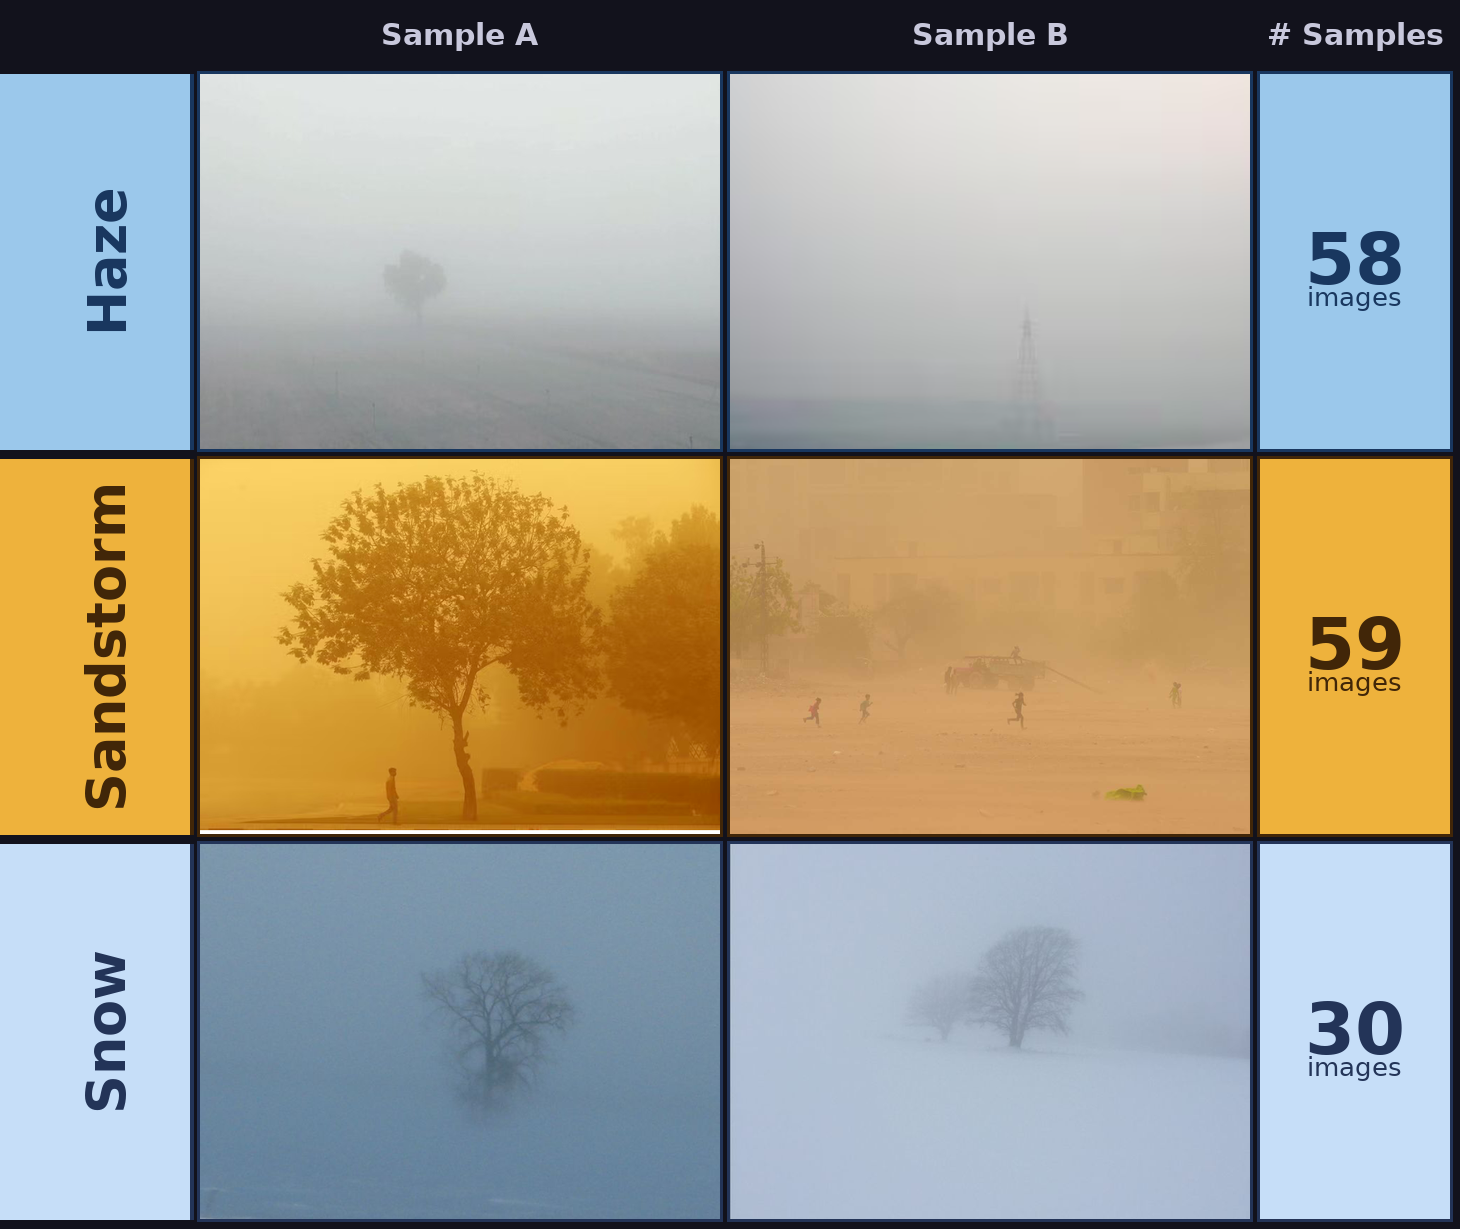
\includegraphics[width=0.92\textwidth]{images/style_ref_grid.png}
\caption{Representative style reference samples from the curated library across the three atmospheric domains. \textbf{Haze} (top row): open-field low-visibility scenes with no dominant foreground objects, characteristic grey-white scattering. \textbf{Sandstorm} (middle row): golden-amber particle diffusion with progressively obscured background; both samples pass the foreground-object test. \textbf{Snow} (bottom row): falling-snow and surface-accumulation variants selected after pipeline testing to maximise colour-temperature shift without leaking tree or building silhouettes into generated agricultural content.}
\label{fig:style_ref_samples}
\end{figure}

\FloatBarrier
% =====================================================
\section{Stage 1: Clean Scene Generation}
\label{sec:stage1_clean}

\noindent Stage~1 uses SDXL~\cite{podell2023sdxlimprovinglatentdiffusion} to generate clean, clear-weather agricultural and rural scenes that will serve as content images for all subsequent stages.

\paragraph{Prompt Design}
Ten base prompts were written to cover the diversity of aerial, agricultural, and rural scene types relevant to drone imagery:
\begin{enumerate}
    \item ``Aerial view of a wheat field with a red tractor plowing rows''
    \item ``Close-up of horses running across an open pasture, clear sky''
    \item ``A greenhouse complex with rows of vegetables, sunny afternoon''
    \item ``Sheep herd on a hillside with stone fences, rolling countryside''
    \item ``Corn maze with a scarecrow, harvest season, golden hour''
    \item ``Flooded rice paddies reflecting blue sky, aerial perspective''
    \item ``Vineyard rows on a gentle slope, green canopy, rural road''
    \item ``Sunflower field from above, geometric pattern, clear day''
    \item ``A farmhouse with a red barn, chicken coop, open meadow''
    \item ``Dirt road through an orchard, apple trees in full leaf, summer''
\end{enumerate}

\paragraph{Generation Parameters}
SDXL was run at $896\times896$ resolution with 40 DDIM steps, guidance scale 7.5, and 5 random seeds per prompt — producing 50 candidate scenes. Manual selection retained the 45 highest-quality scenes (rejecting 5 that had structural artifacts or semantically implausible geometry). These 45 scenes form the clean scene pool used throughout the pipeline.

\begin{figure}[!ht]
    \centering
    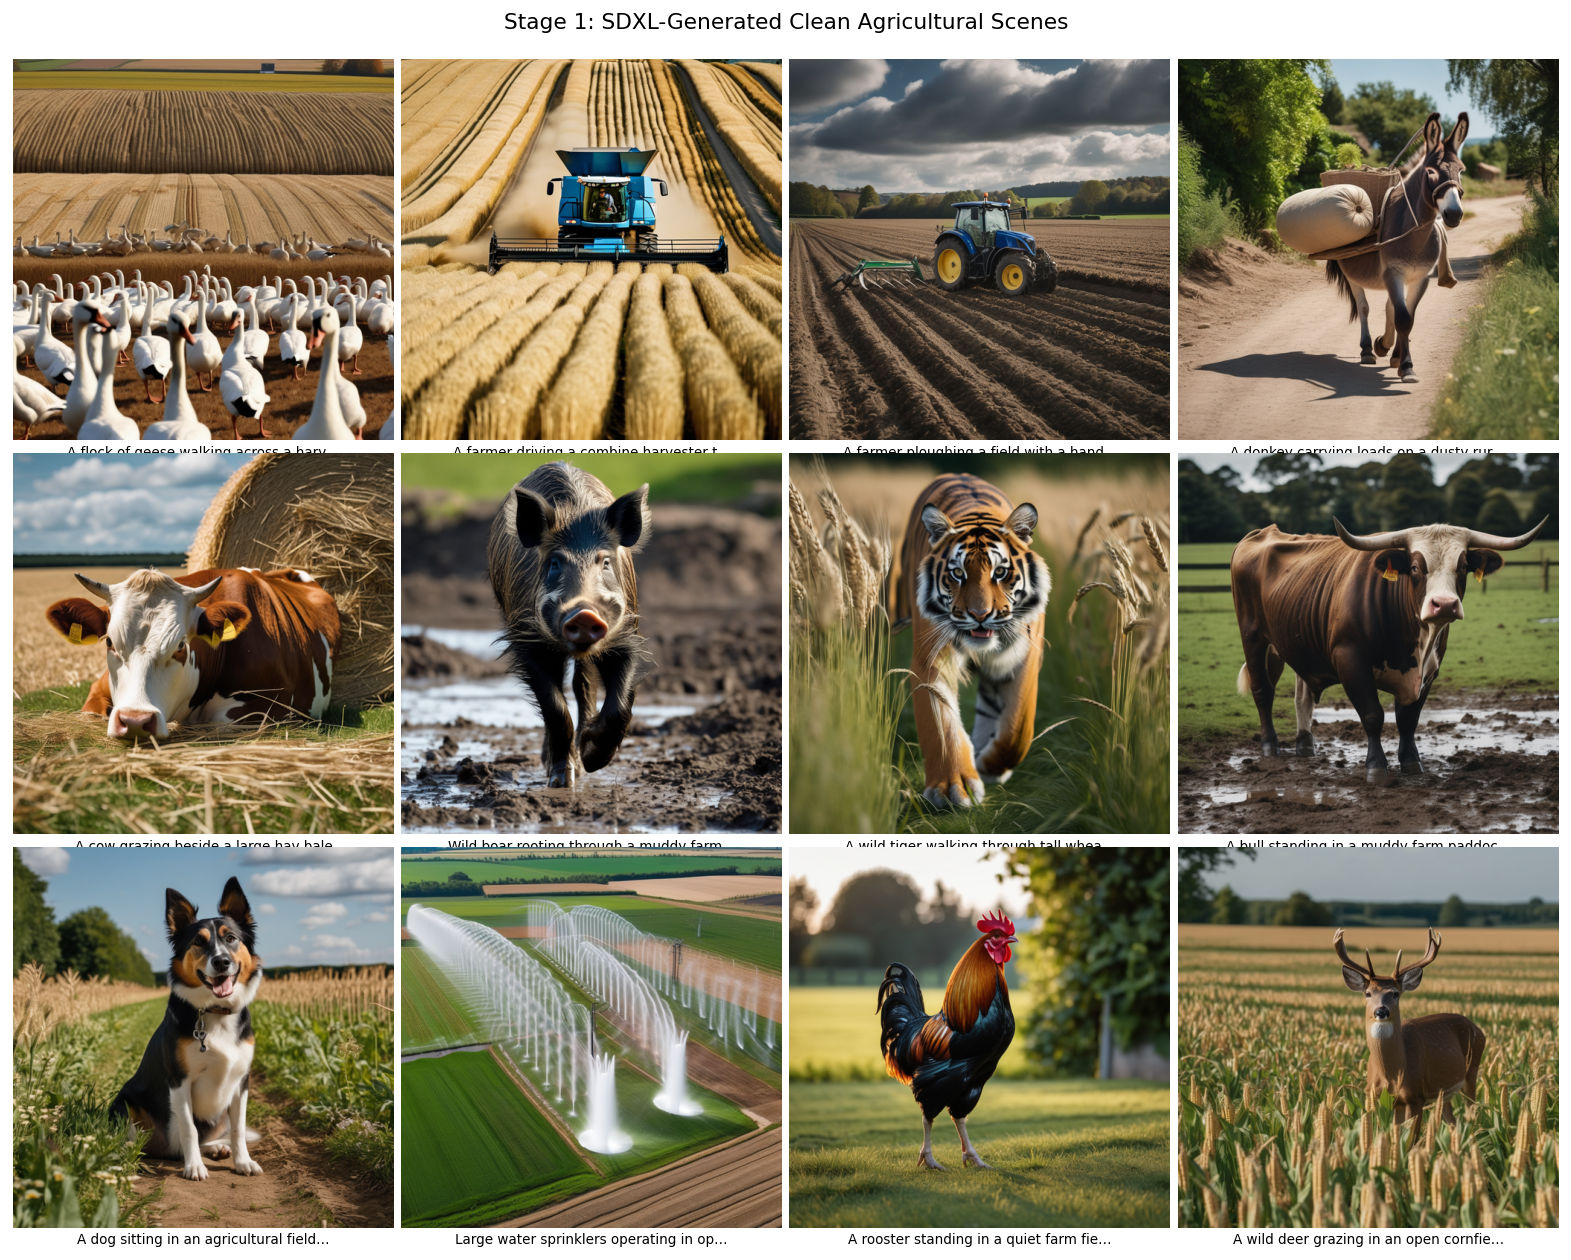
\includegraphics[width=0.85\linewidth]{images/agricultural_prompts_grid.png}
    \caption{Representative clean agricultural scenes generated in Stage~1. These 45 scenes form the content pool for all atmospheric style applications in Stages~2 and~3.}
    \label{fig:agricultural_prompts_grid}
\end{figure}

\FloatBarrier
% =====================================================
\section{Style Transfer Configurations (V1--V4)}
\label{sec:stage2_style}

\noindent Stage~2 applies an atmospheric style transfer pass on each clean scene. Four progressively refined pipeline configurations (V1--V4) were developed and compared, building on each other iteratively. V1 and V2 use style transfer alone; V3 and V4 additionally invoke the Stage~3 physics compositor, making them full three-stage pipeline variants. V4 was subsequently discarded due to destructive interference artefacts; V3 is the primary physics-grounded baseline. Table~\ref{tab:version_naming} provides the formal nomenclature for all versions; Table~\ref{tab:stage2_evolution} summarises how the Stage~2 architecture evolved. All version codes throughout this chapter refer to Table~\ref{tab:version_naming}.

\begin{table}[htbp]
\centering
\caption{Stage~2 architecture evolution across pipeline versions. CLIP confidence (ViT-L-14) is the mean softmax score on generated outputs — lower = stronger domain shift from clean. V4 was abandoned due to destructive interference artefacts. V3 and V9 are the final pipelines used in evaluation.}
\label{tab:stage2_evolution}
\resizebox{\textwidth}{!}{%
\small
\setlength{\tabcolsep}{4.5pt}
\begin{tabular}{lcccc}
\toprule
\textbf{Component} & \textbf{V1} & \textbf{V2}
  & \cellcolor{green!8}\textbf{V3 (Final)}
  & \cellcolor{teal!8}\textbf{V9 (Best)} \\
\midrule
IP-Adapter blocks
  & All (down+mid+up) & up$_{0}$+up$_{1}$
  & \cellcolor{green!8}up$_{0}$+up$_{1}$
  & \cellcolor{teal!8}up$_{0}$+up$_{1}$+mid \\
IP scale
  & 0.50 & 0.75
  & \cellcolor{green!8}0.85--0.88 & \cellcolor{teal!8}0.95 \\
img2img strength
  & 0.65 & 0.65
  & \cellcolor{green!8}0.70--0.74 & \cellcolor{teal!8}--- (pure t2i) \\
CSD guidance
  & $\checkmark$\ ($\eta$=0.18) & $\checkmark$\ ($\eta$=0.18)
  & \cellcolor{green!8}$\times$\ (removed) & \cellcolor{teal!8}$\checkmark$\ ($\eta$=0.25, $w$=1.5) \\
Spatial noise map
  & $\checkmark$ & $\times$
  & \cellcolor{green!8}$\times$ & \cellcolor{teal!8}$\times$ \\
Content subtraction
  & $\times$ & $\times$
  & \cellcolor{green!8}$\times$
  & \cellcolor{teal!8}$\checkmark$\ (CLIP ZS, $\alpha$=0.45) \\
Stage~3 compositor
  & Koschmieder & Koschmieder
  & \cellcolor{green!8}Koschmieder + high$\beta$
  & \cellcolor{teal!8}haze$\rightarrow$V3 / sand$\rightarrow$V5 Mie / snow$\rightarrow$V7 \\
\midrule
CLIP confidence $\downarrow$
  & 0.299 & 0.317
  & \cellcolor{green!8}\textbf{0.274}
  & \cellcolor{teal!8}\textbf{0.228} \\
Status
  & Superseded & Superseded
  & \cellcolor{green!8}Final dataset
  & \cellcolor{teal!8}Best pipeline \\
\bottomrule
\end{tabular}
}
\end{table}


\FloatBarrier
% -------------------------------------------------------
\begin{table}[htbp]
\centering
\caption{Version naming reference: internal codes, descriptions, and proposed formal names. All subsequent sections use the internal codes (V0--V9); this table provides the full nomenclature for cross-referencing.}
\label{tab:version_naming}
\small
\setlength{\tabcolsep}{5pt}
\renewcommand{\arraystretch}{1.3}
\begin{tabular}{@{}llp{6.2cm}@{}}
\toprule
\textbf{Code} & \textbf{Internal Description} & \textbf{Proposed Formal Name} \\
\midrule
V0  & InstantStyle + CSD Guidance                    & CSD-Guided Latent Optimisation \\
V1  & Global Style Injection + Depth-Modulated Noise & Depth-Aware Global Haze Injection \\
V2  & Style-Block Injection + Perceptual Guidance    & Block-Selective Perceptual Style Transfer \\
V3  & Style-Block Injection + Koschmieder            & Physics-Grounded Atmospheric Compositing \\
V4  & CSD + Koschmieder (Discarded)                  & CSD--Physics Hybrid Fusion (ablated) \\
V5  & Sandstorm Wavelength-Dependent Scattering      & Mie-Scattering Sandstorm Synthesis \\
V6  & Procedural Snowfall Simulation                 & Procedural Snowfall Particle Rendering \\
V7  & Snow Accumulation Modelling                    & Layered Winter Scene Synthesis \\
V9  & CLIP Subtraction + Koschmieder                 & Semantic-Decoupled Atmospheric Style Transfer \\
\bottomrule
\end{tabular}
\end{table}

\FloatBarrier
% -------------------------------------------------------
\subsection{V1: Global Style Injection with Depth-Modulated Noise}
\label{sec:v1}

\noindent V1~(Table~\ref{tab:version_naming}) was the starting point: IP-Adapter with all-block injection (not block-selective) combined with a spatially non-uniform noise map. The rationale was that all-block injection provides stronger style transfer, and the spatial noise map compensates for the lack of depth-awareness by explicitly modulating noise intensity by scene depth.

\paragraph{Configuration}
\begin{itemize}
    \item IP-Adapter injection: ALL blocks (down, mid, up), scale = 0.50.
    \item Spatial noise map: $s(x) = 0.55 + 0.20 \cdot w_\mathrm{depth}(x)$, where $w_\mathrm{depth}(x)$ is the normalised inverse depth (deeper $\rightarrow$ higher noise addition).
    \item CSD guidance: $\eta = 0.18$, applied every 3 steps.
    \item Style references: 3 domains — haze, sandstorm, snow.
\end{itemize}

\paragraph{Observations}
V1~(Table~\ref{tab:version_naming}) produced visually appealing atmospheric scenes but retained layout leakage and semantic drift from all-block injection. The ViT-L-14 confidence dropped from 0.3412 to 0.2978, indicating a modest domain shift.

\begin{figure}[htbp]
    \centering
    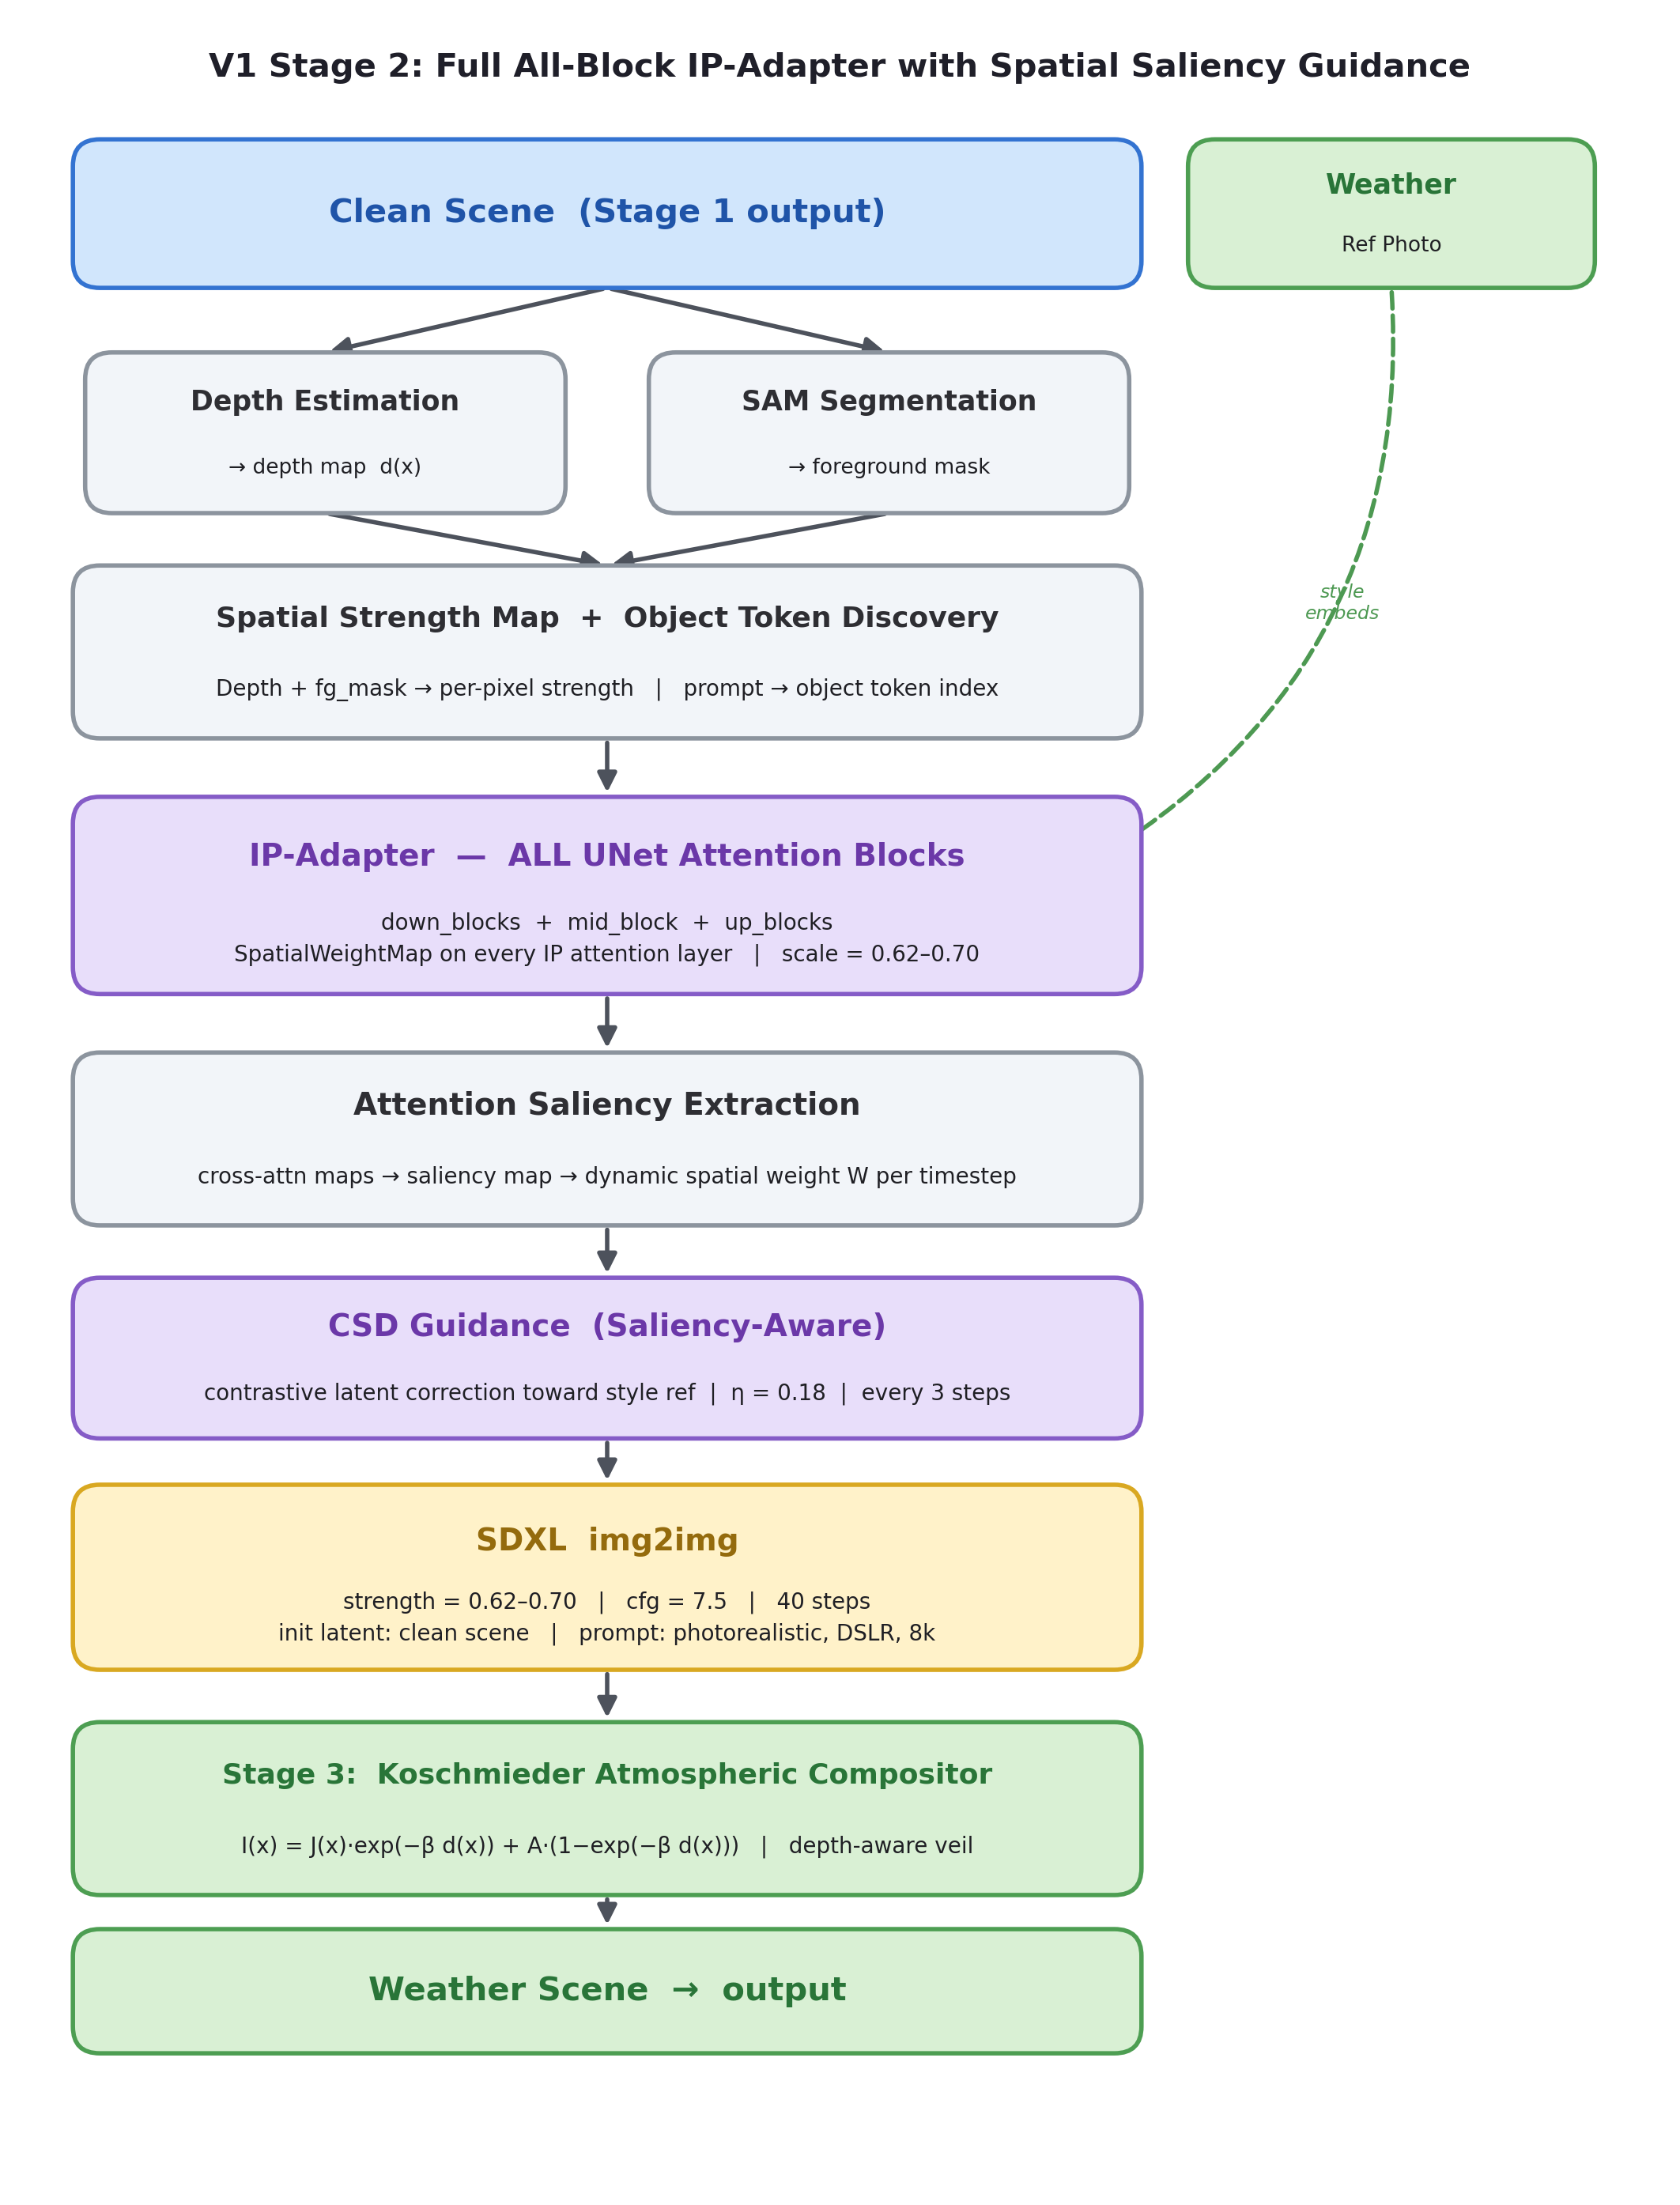
\includegraphics[width=0.82\linewidth]{images/arch_v1_stage2.png}
    \caption{V1 Stage~2 architecture. IP-Adapter injects style features into \emph{all} UNet blocks (\texttt{down\_blocks}, \texttt{mid\_block}, \texttt{up\_blocks}) at a uniform scale of 0.50. A spatially-varying noise map modulates denoising strength per pixel, and CSD gradient guidance is applied every 3 denoising steps. The key failure mode --- semantic leakage from the \texttt{mid\_block} (which encodes object identity) into the generated content --- motivated the block-selective injection approach adopted in V2 and V3. (Figure adapted from the Phase~2 Pipeline Architecture reference document.)}
    \label{fig:arch_v1_stage2}
\end{figure}

\FloatBarrier
% -------------------------------------------------------
\subsection{V2: Style-Block Injection with Perceptual Guidance}
\label{sec:v2}

\noindent V2~(Table~\ref{tab:version_naming}) switched to the block-selective InstantStyle injection (matching the proposed method from Chapter~\ref{chap:adaptive_proposed}) and increased the injection scale to compensate for the narrower injection scope.

\paragraph{Configuration}
\begin{itemize}
    \item IP-Adapter injection: \texttt{up\_blocks.0} and \texttt{up\_blocks.1} only (block-selective).
    \item Style injection scale: 0.75 (haze), 0.78 (sandstorm), 0.72 (snow).
    \item Img2img strength (denoising ratio): 0.62--0.70.
    \item CSD guidance: $\eta = 0.15$--$0.18$ (domain-specific), every 3 steps.
\end{itemize}

\paragraph{Observations}
V2~(Table~\ref{tab:version_naming}) preserved content semantic structure significantly better than V1. The ViT-L-14 zero-shot confidence on V2~(Table~\ref{tab:version_naming}) outputs was 0.3162 — actually slightly \emph{higher} than V1 (0.2978), indicating that V2's style transfer was more semantically transparent: the images looked more like stylised clean scenes and less like genuinely shifted domains. However, the Top-1 classification accuracy on V2 outputs was high: 93.3\% on haze, 94.1\% on sandstorm, 99.3\% on snow, and 96.0\% overall. This confirmed a known issue: block-selective injection produces high-quality-looking style transfer but the feature-space shift is insufficient for training robust vision models.

\FloatBarrier
% -------------------------------------------------------
\subsection{V3: Style-Block Injection with Physics Compositing}
\label{sec:v3}

\noindent V3~(Table~\ref{tab:version_naming}) was motivated by the observation that CSD guidance, while improving visual realism, does not meaningfully increase the feature-space domain shift beyond what InstantStyle alone achieves. Removing CSD guidance and using a minimal, generic text prompt (rather than a detailed agricultural description) was expected to reduce the model's tendency to ``fight back'' against the style transfer with its own prior knowledge of what agricultural scenes look like.

\paragraph{Configuration}
\begin{itemize}
    \item IP-Adapter injection: \texttt{up\_blocks.0} and \texttt{up\_blocks.1} only.
    \item Style injection scale: 0.85 (haze), 0.88 (sandstorm), 0.82 (snow) — higher than V2.
    \item Img2img strength: 0.72--0.74 (higher denoising ratio than V2, allowing more style influence).
    \item CSD guidance: \textbf{none}.
    \item Text prompt: minimal generic prompt (e.g., ``outdoor scene, atmospheric'') rather than detailed agricultural description.
    \item Koschmieder Stage~3 compositor: applied after style transfer (see Section~\ref{sec:stage3_physics}).
\end{itemize}

\paragraph{Observations}
V3~(Table~\ref{tab:version_naming}) achieved the strongest feature-space shift. Top-1 classification accuracy on V3~(Table~\ref{tab:version_naming}) outputs was 67.2\% (ViT-L-14) and 67.4\% (ViT-H-14) — well below the near-perfect accuracy on clean scenes and below V2's 96.0\%/95.3\%. The ViT-L-14 zero-shot confidence was 0.2744 — the lowest of all three versions, and noticeably below the clean scene confidence of 0.3416. The removal of CSD guidance made the images slightly less visually polished (some colour banding and texture inconsistency that CSD would have smoothed), but this was an acceptable trade-off for the stronger domain shift. V3 became the primary training data source for the downstream experiments.

\begin{figure}[htbp]
    \centering
    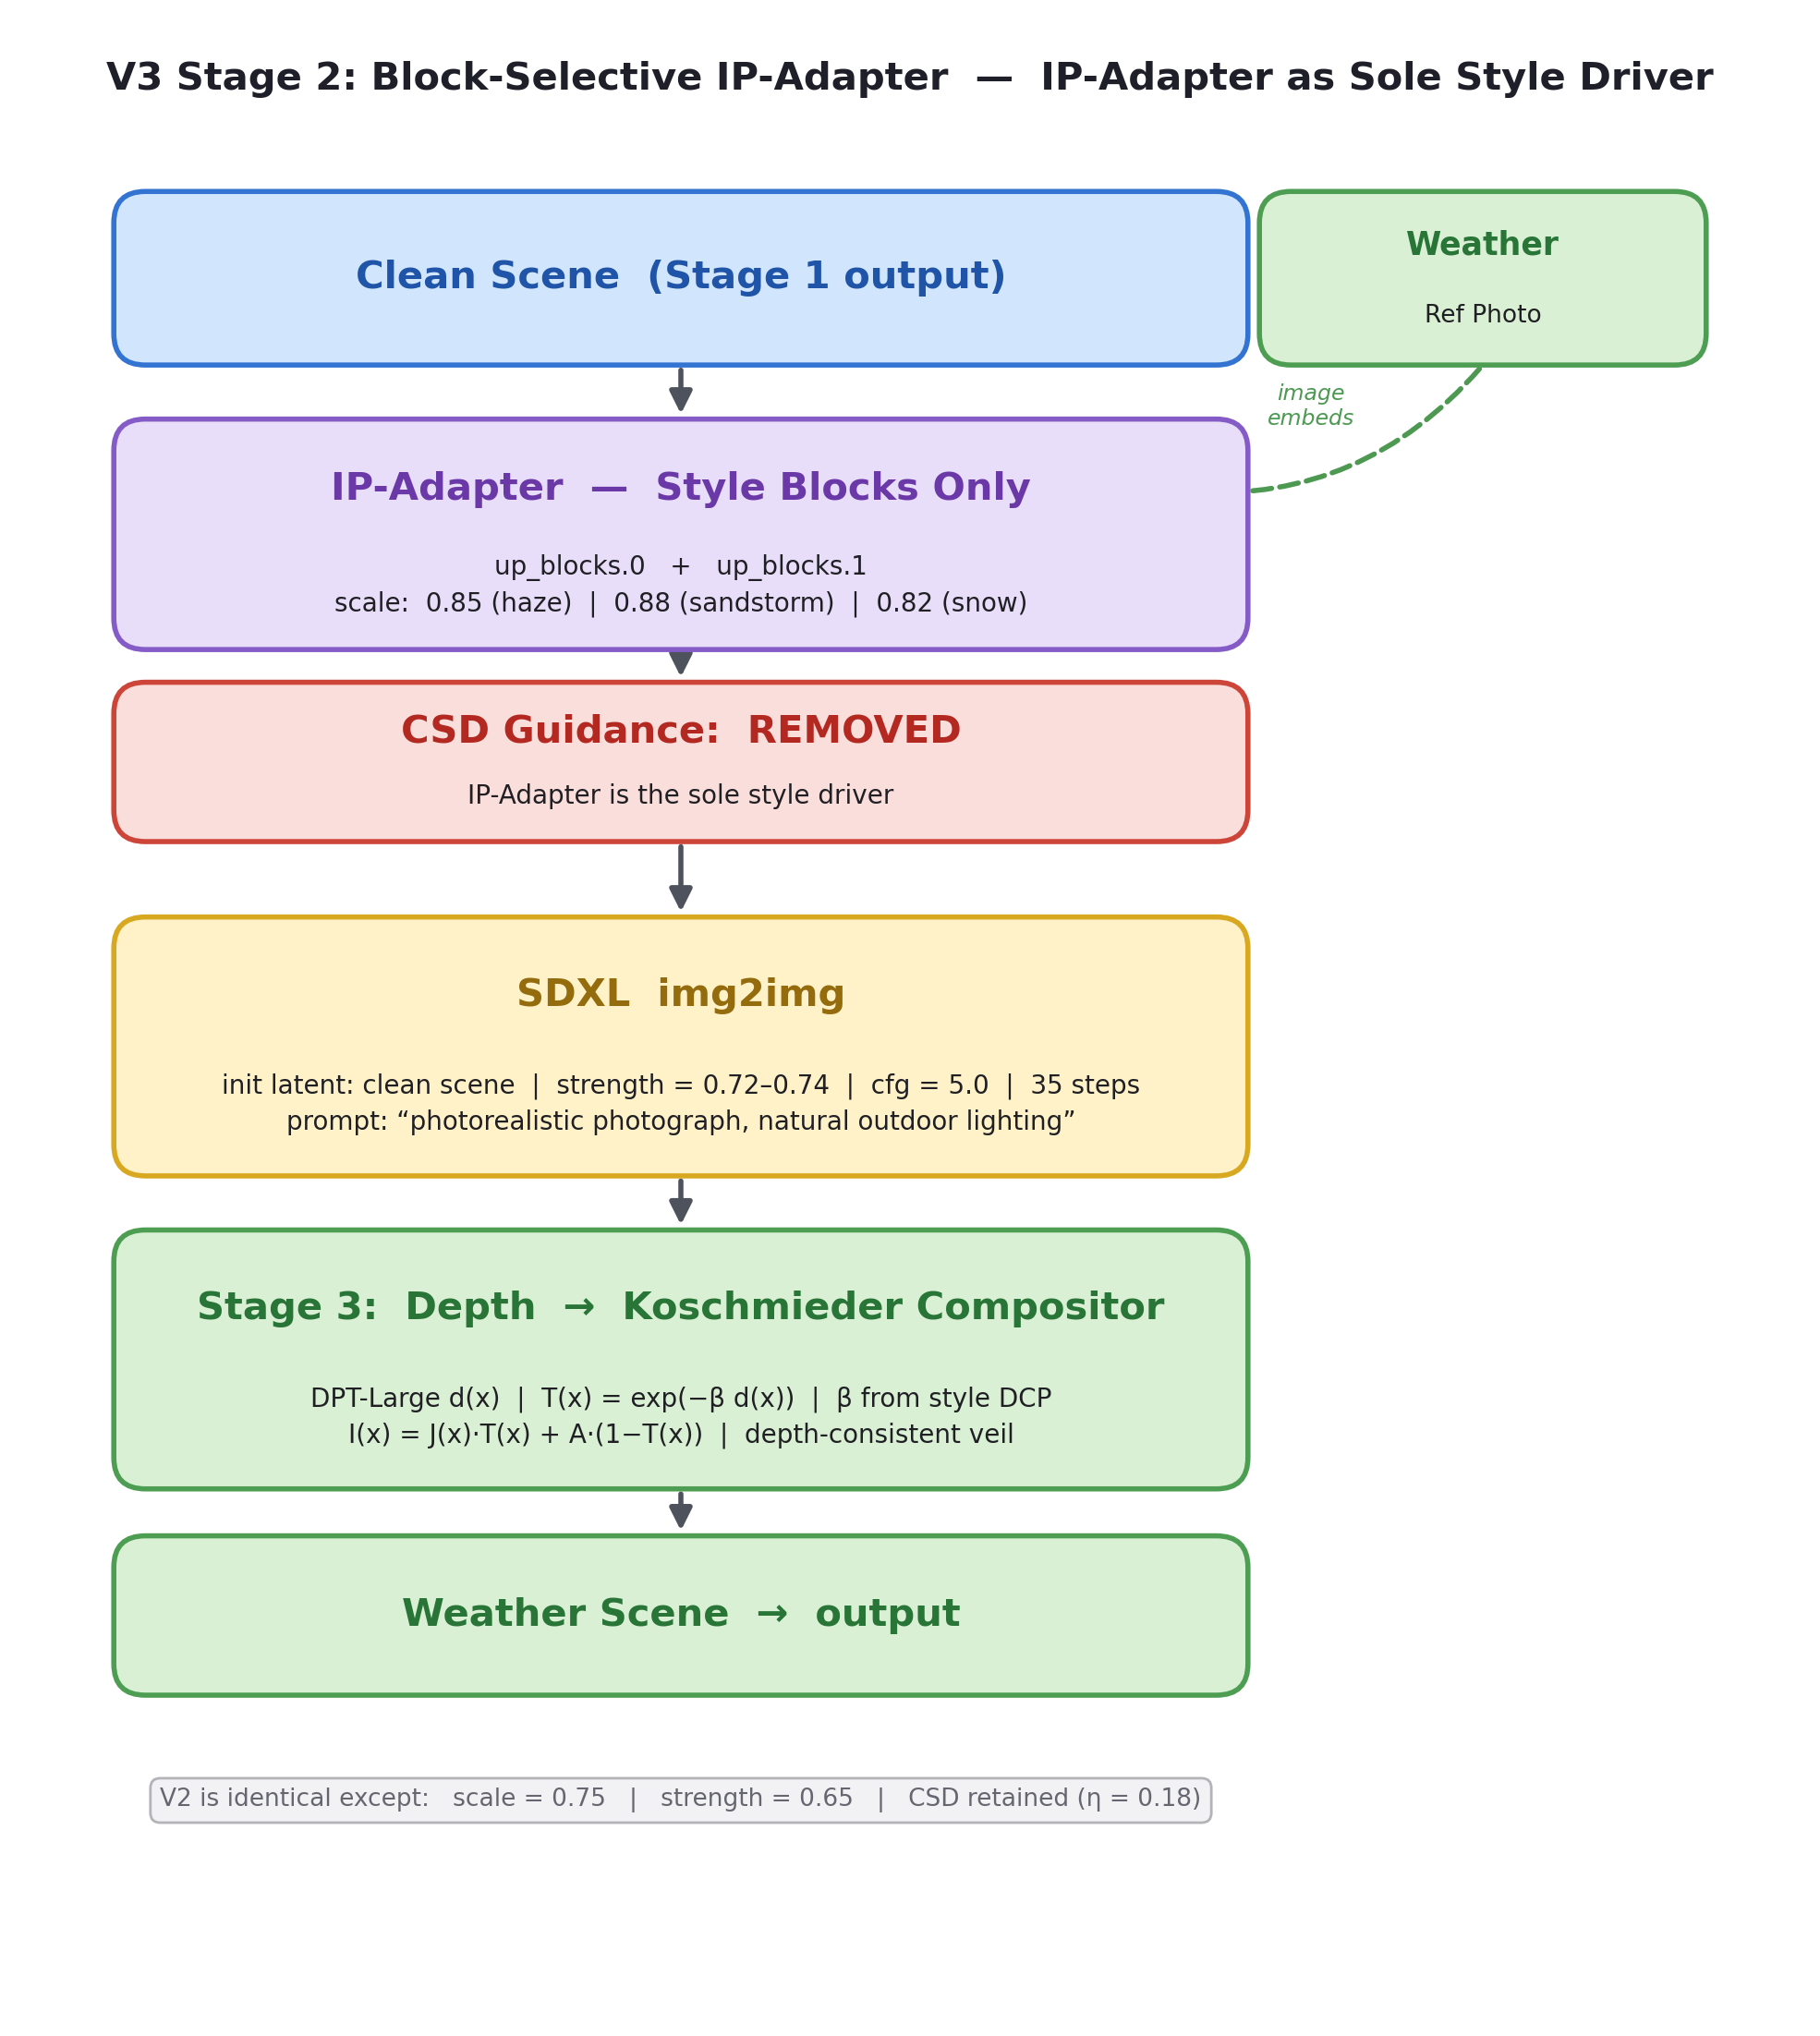
\includegraphics[width=0.80\linewidth]{images/arch_v3_stage2.png}
    \caption{V3 Stage~2 architecture (final pipeline). Block injection is restricted to \texttt{up\_blocks.0} and \texttt{up\_blocks.1} (scale\,=\,0.85--0.88 per domain), eliminating semantic leakage from the structural blocks. CSD guidance is \textbf{removed}: IP-Adapter is the sole style driver. A minimal generic prompt (``photorealistic photograph, natural outdoor lighting'') is used to prevent SDXL's text conditioning from competing with the image-style signal. Higher denoising strength (0.72--0.74) commits more fully to weather style than V2. The V2 architecture is identical except for lower scale (0.75), lower denoising strength (0.65), and CSD guidance retained ($\eta=0.18$). (Figure adapted from the Phase~2 Pipeline Architecture reference document.)}
    \label{fig:arch_v3_stage2}
\end{figure}

\begin{figure}[htbp]
    \centering
    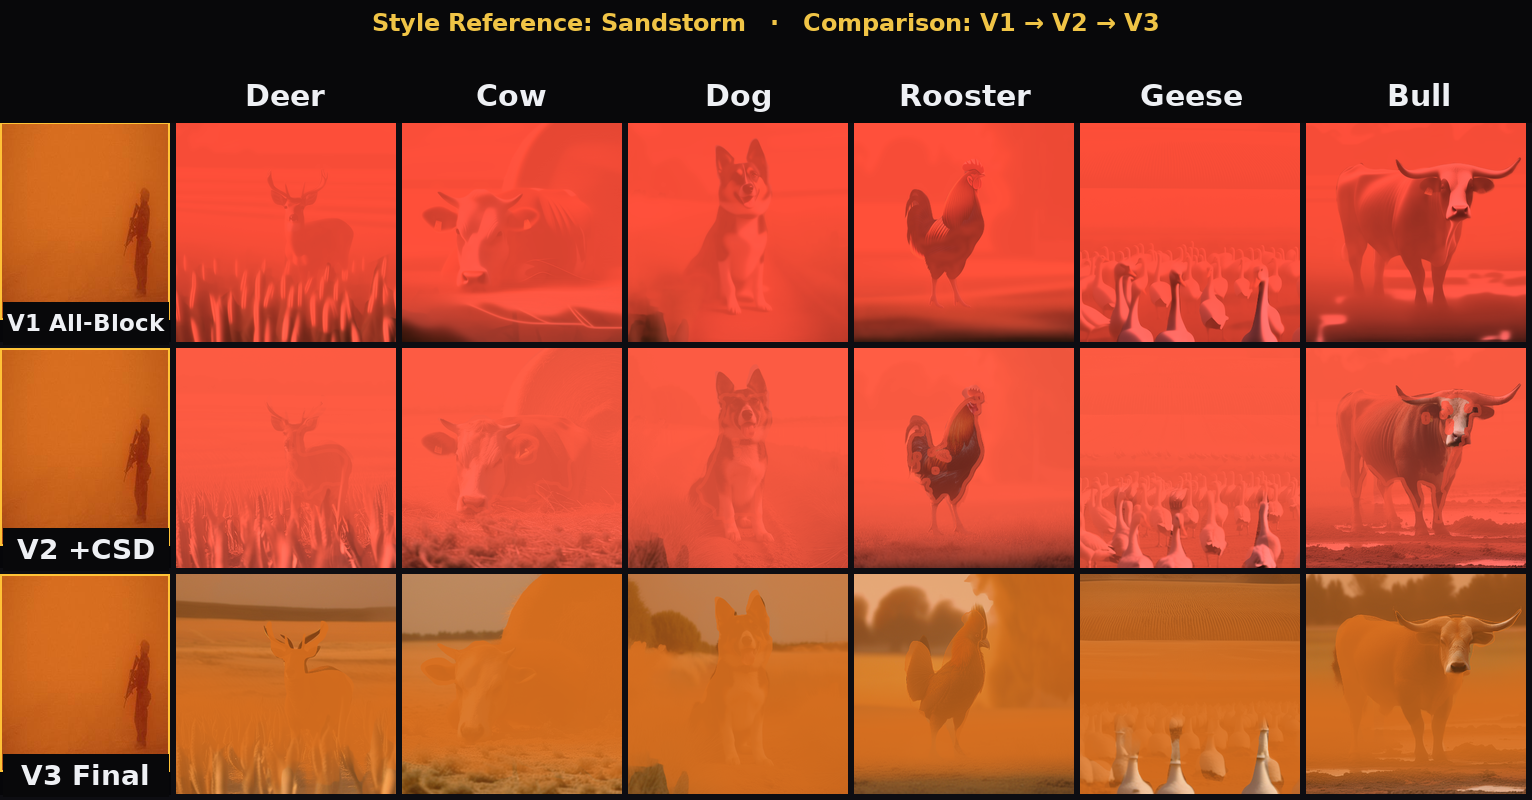
\includegraphics[width=0.97\linewidth]{images/v1_v2_v3_comparison.png}
    \caption{Pipeline comparison: V1 (all-block injection), V2 (block-selective + CSD), and V3 (block-selective, no CSD) applied to six content prompts using the same sandstorm style reference. Each row shows outputs from one pipeline version; columns are different agricultural scenes. V3 achieves the strongest atmospheric character.}
    \label{fig:v1_v2_v3_comparison}
\end{figure}

\paragraph{Dataset Scale}
45 clean scenes $\times$ 3 atmospheric styles $\times$ 3 versions = 405 images total. The full V3 dataset (405 images across all domains) was used for Experiments 1--3.

\paragraph{V3-HighBeta Variant}
\label{sec:v3_highbeta}
To probe the sensitivity of depth-coherence to the Koschmieder scattering coefficient, a single ablation variant of V3 --- designated \textbf{V3-HighBeta} --- was generated using twice the nominal scattering coefficient ($\beta_{\mathrm{HB}} = 2\beta_{\mathrm{V3}}$). All other V3 hyperparameters were held constant; only the Koschmieder compositor received the elevated $\beta$ value. The stronger extinction coefficient substantially increases the physical haze density at depth, producing images where distant objects are almost entirely occluded. This variant was not used as training data for downstream experiments but was included in the metrics study (Section~\ref{sec:proposed_metrics}) to establish how increasing the scattering coefficient $\beta$ degrades subject visibility, serving as an upper-bound reference for atmospheric strength.

\FloatBarrier
% -------------------------------------------------------
\subsection{V4: CSD + Koschmieder (Discarded)}
\label{sec:v4_discarded}

\noindent V4~(Table~\ref{tab:version_naming}) was an attempt to combine V3's Koschmieder physics compositor with CSD guidance reintroduced at the latent level, testing whether active perceptual correction could further refine the style signal on top of physics-grounded compositing.

\noindent Qualitative inspection of the V4~(Table~\ref{tab:version_naming}) outputs immediately revealed severe artefacts across all three atmospheric domains. Haze samples exhibited pronounced red/cyan chromatic aberration — bright red halos around every subject edge and cyan fringing in shadows, resembling a 3D anaglyph image viewed without glasses. In several farmland samples, content drifted entirely (SDXL hallucinated unrelated scenery such as waterfalls). Sandstorm samples showed teal--orange colour channel separation, producing a duotone or thermal-imaging appearance rather than the warm, uniform particulate characteristic of sandstorm imagery. Snow samples displayed a strong green cast with no visible snow effect — CSD had pushed the latents in the opposite direction from the cold white/blue snow style reference.

\paragraph{Why the failure occurs}
CSD applies gradient corrections at the latent level every 3 denoising steps, while IP-Adapter injects style via cross-attention simultaneously. At V3's high denoising strength (0.78--0.85), approximately 27 active denoising steps remain, yielding $\sim$9 CSD corrections per image. These corrections compound: the accumulated colour shifts manifest as chromatic aberration and channel separation visible in every domain. The two objectives compete directly — IP-Adapter pulls cross-attention features toward the weather style while CSD simultaneously pushes latents toward the CSD style descriptor. At this denoising strength, neither wins cleanly, producing destructive interference. This contrasts with V2, where the weaker denoising strength (0.65) permitted partial coexistence of the two signals.

\noindent V4~(Table~\ref{tab:version_naming}) was discarded after the qualitative inspection. The artefacts are visually unambiguous and constitute strong evidence that the V3 design choice — IP-Adapter as the sole style driver with no competing gradient objectives — is the correct architecture for weather transfer at committed denoising strengths.

\FloatBarrier
% =====================================================
\section{Stage 3: Physics-Grounded Atmospheric Compositor}
\label{sec:stage3_physics}

\noindent Stage~3 takes each style-transferred image from Stage~2 and applies a depth-aware physics compositor that enforces the Koschmieder atmospheric scattering law~\cite{koschmieder1924theorie}. This is the key innovation of the proposed pipeline: rather than asking a generative model to impose physical constraints (which the preceding style transfer experiments showed to be unreliable), the physics is applied as a deterministic post-processor.

\FloatBarrier
% -------------------------------------------------------
\subsection{Koschmieder Atmospheric Scattering Model}
\label{sec:koschmieder}

\noindent The Koschmieder model~\cite{koschmieder1924theorie} describes how an image $I(x)$ of a scene with radiance $J(x)$ is affected by atmospheric scattering:
\begin{equation}
    I(x) = J(x) \cdot T(x) + A \cdot (1 - T(x)),
    \label{eq:koschmieder}
\end{equation}
where:
\begin{itemize}
    \item $T(x) = \exp(-\beta \cdot D(x))$ is the \textbf{transmission map}: the fraction of scene radiance that survives to the camera.
    \item $D(x)$ is the scene depth at pixel $x$.
    \item $\beta$ is the \textbf{scattering coefficient}: larger $\beta$ means denser atmosphere.
    \item $A$ is the \textbf{atmospheric light} (airlight): the colour of the medium itself (white for haze, warm yellow-brown for sandstorm, blue-white for snow).
\end{itemize}

\noindent When $D(x)$ is large (distant object), $T(x) \rightarrow 0$ and $I(x) \rightarrow A$ — the object disappears into the atmospheric medium. When $D(x)$ is small (close object), $T(x) \rightarrow 1$ and $I(x) \rightarrow J(x)$ — the object is seen clearly. This is exactly the depth-dependent attenuation that was missing from all the style-transfer approaches in earlier experiments.

\FloatBarrier
% -------------------------------------------------------
\subsection{Depth Estimation with Intel DPT-Large}
\label{sec:dpt_depth}

\noindent Per-scene depth maps $D(x)$ were estimated using Intel DPT-Large~\cite{ranftl2021dpt}, a transformer-based monocular depth estimator. DPT-Large was run on each Stage~2 style-transferred image to produce a normalised depth map in $[0, 1]$. The scattering coefficient $\beta$ and atmospheric light $A$ were set per-domain:

\begin{itemize}
    \item \textbf{Haze:} $\beta = 1.5$--$3.0$, $A = [0.95, 0.95, 0.95]$ (near-white).
    \item \textbf{Sandstorm:} $\beta = 2.0$--$4.0$, $A = [0.90, 0.80, 0.60]$ (warm amber).
    \item \textbf{Snow:} $\beta = 1.0$--$2.5$, $A = [0.92, 0.94, 0.98]$ (cool blue-white).
\end{itemize}

\noindent These values were derived from the Dark Channel Prior method~\cite{he2009dark}, which estimates $\beta$ and $A$ from statistics of the style reference photographs in the curated dataset.

\FloatBarrier
% -------------------------------------------------------
\subsection{Three-Step Compositing Pipeline}
\label{sec:compositing}

\noindent The Stage~3 compositor applies three sequential operations:

\paragraph{Step 1: Atmospheric Veil (Koschmieder)}
The transmission map $T(x) = \exp(-\beta \cdot D(x))$ is computed from the DPT-Large depth map. Equation~\ref{eq:koschmieder} is then applied pixel-wise: $I(x) = J(x) \cdot T(x) + A \cdot (1 - T(x))$.

\paragraph{Step 2: Edge Dissolution}
Real atmospheric scenes exhibit softening of high-frequency edges in proportion to depth. A depth-weighted Gaussian blur is applied: $\sigma(x) = \sigma_\mathrm{max} \cdot (1 - T(x))$. Pixels in deeply attenuated regions (low $T$) receive more blur; foreground pixels receive minimal blur.

\paragraph{Step 3: Colour and Saturation Shift}
Atmospheric scattering affects colour channels non-uniformly. A channel-specific saturation reduction is applied, with the magnitude proportional to $(1 - T(x))$: pixels that are more heavily attenuated also receive stronger desaturation toward the atmospheric light colour $A$.

\begin{figure}[htbp]
    \centering
    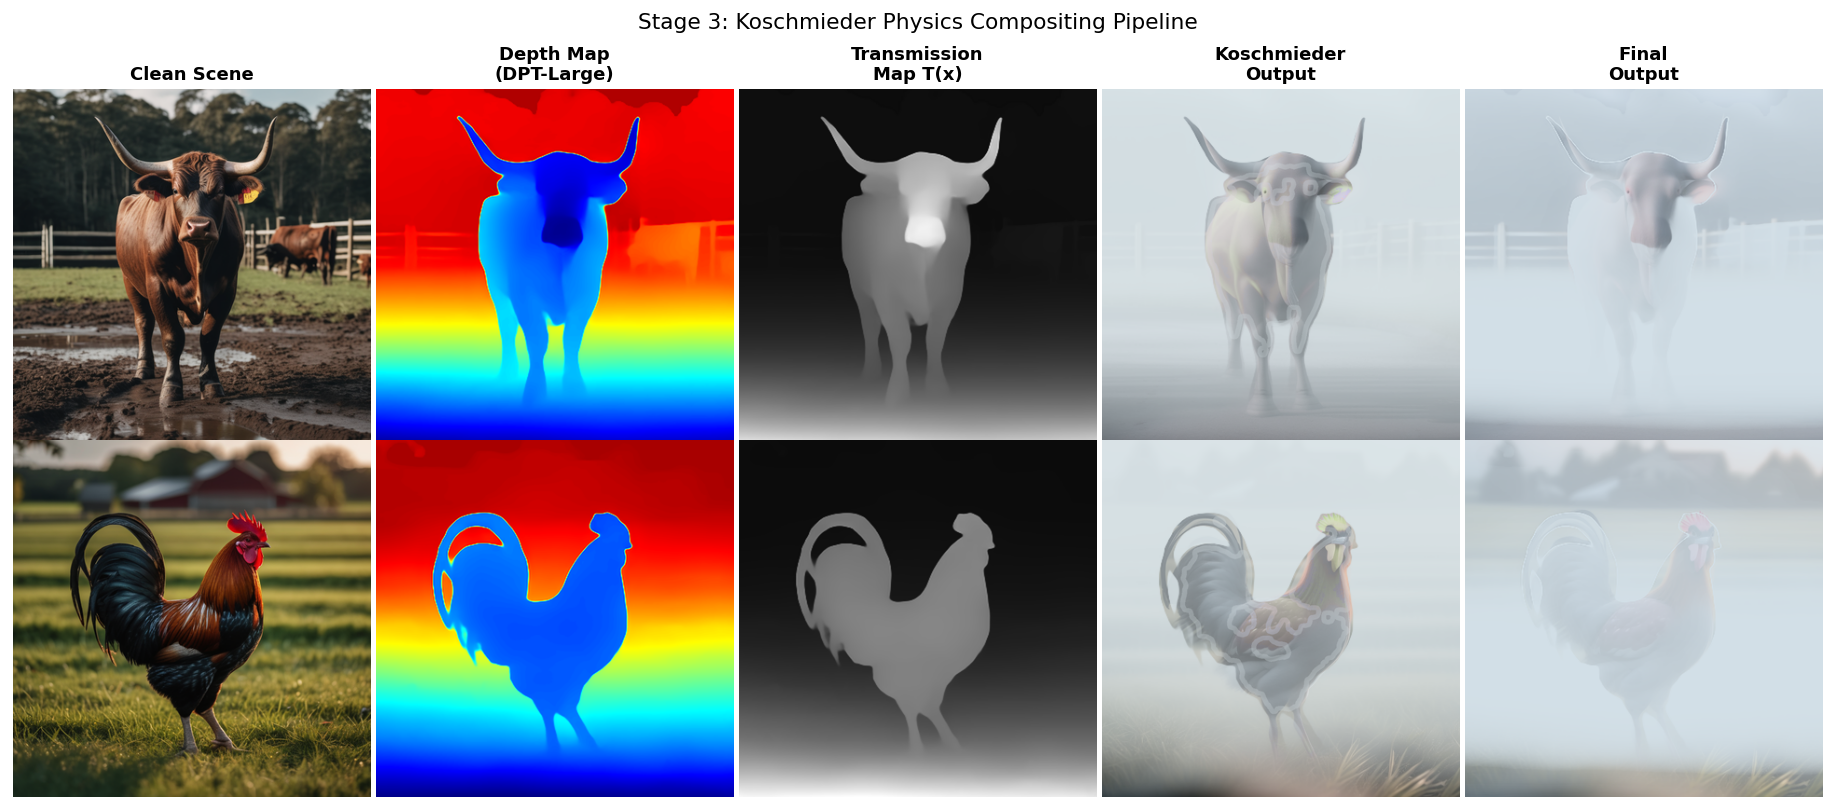
\includegraphics[width=0.97\linewidth]{images/koschmieder_depth_stages.png}
    \caption{Stage~3 physics compositing pipeline for a single example. Top row: clean scene, DPT-Large depth map, computed transmission map. Bottom row: Koschmieder output (Eq.~\ref{eq:koschmieder}), edge-dissolved version, final output with colour shift.}
    \label{fig:koschmieder_depth_stages}
\end{figure}

\FloatBarrier
% =====================================================
\section{KDA-Net: The Learned Compositor Attempt}
\label{sec:kda_net}

\noindent In parallel with the Koschmieder compositor, a learned neural compositor, KDA-Net, was designed and trained. The goal was to replace the hand-tuned Koschmieder parameters ($\beta$, $A$) with a network that learned to predict the appropriate atmospheric compositing parameters from the scene content and style reference, potentially handling cases where the simple Koschmieder model is insufficient (e.g., participating media with wavelength-dependent scattering).

\FloatBarrier
% -------------------------------------------------------
\subsection{Architecture}
\label{sec:kda_arch}

\noindent KDA-Net has two sub-networks:

\begin{itemize}
    \item \textbf{Haze Image Generator (HIG):} Three modules — Texture Encoder (TE), Haze Encoder (HE), and Image Compositor (IC). The HIG takes a clean scene and a haze style reference and outputs a composited hazy image using a learned transmission map $t^\theta$: $I_o = J_n \cdot t^\theta + A \cdot (1 - t^\theta)$, where $\theta$ are the predicted transmission parameters.
    \item \textbf{Haze Authenticator (HA):} Two patch discriminators — Content Identity (CI) and Haze Identity (HI) — that distinguish genuine atmospheric images from KDA-Net composites. The adversarial training was intended to prevent the HIG from producing atmospheric images that are obviously synthetic.
\end{itemize}

\begin{figure}[htbp]
    \centering
    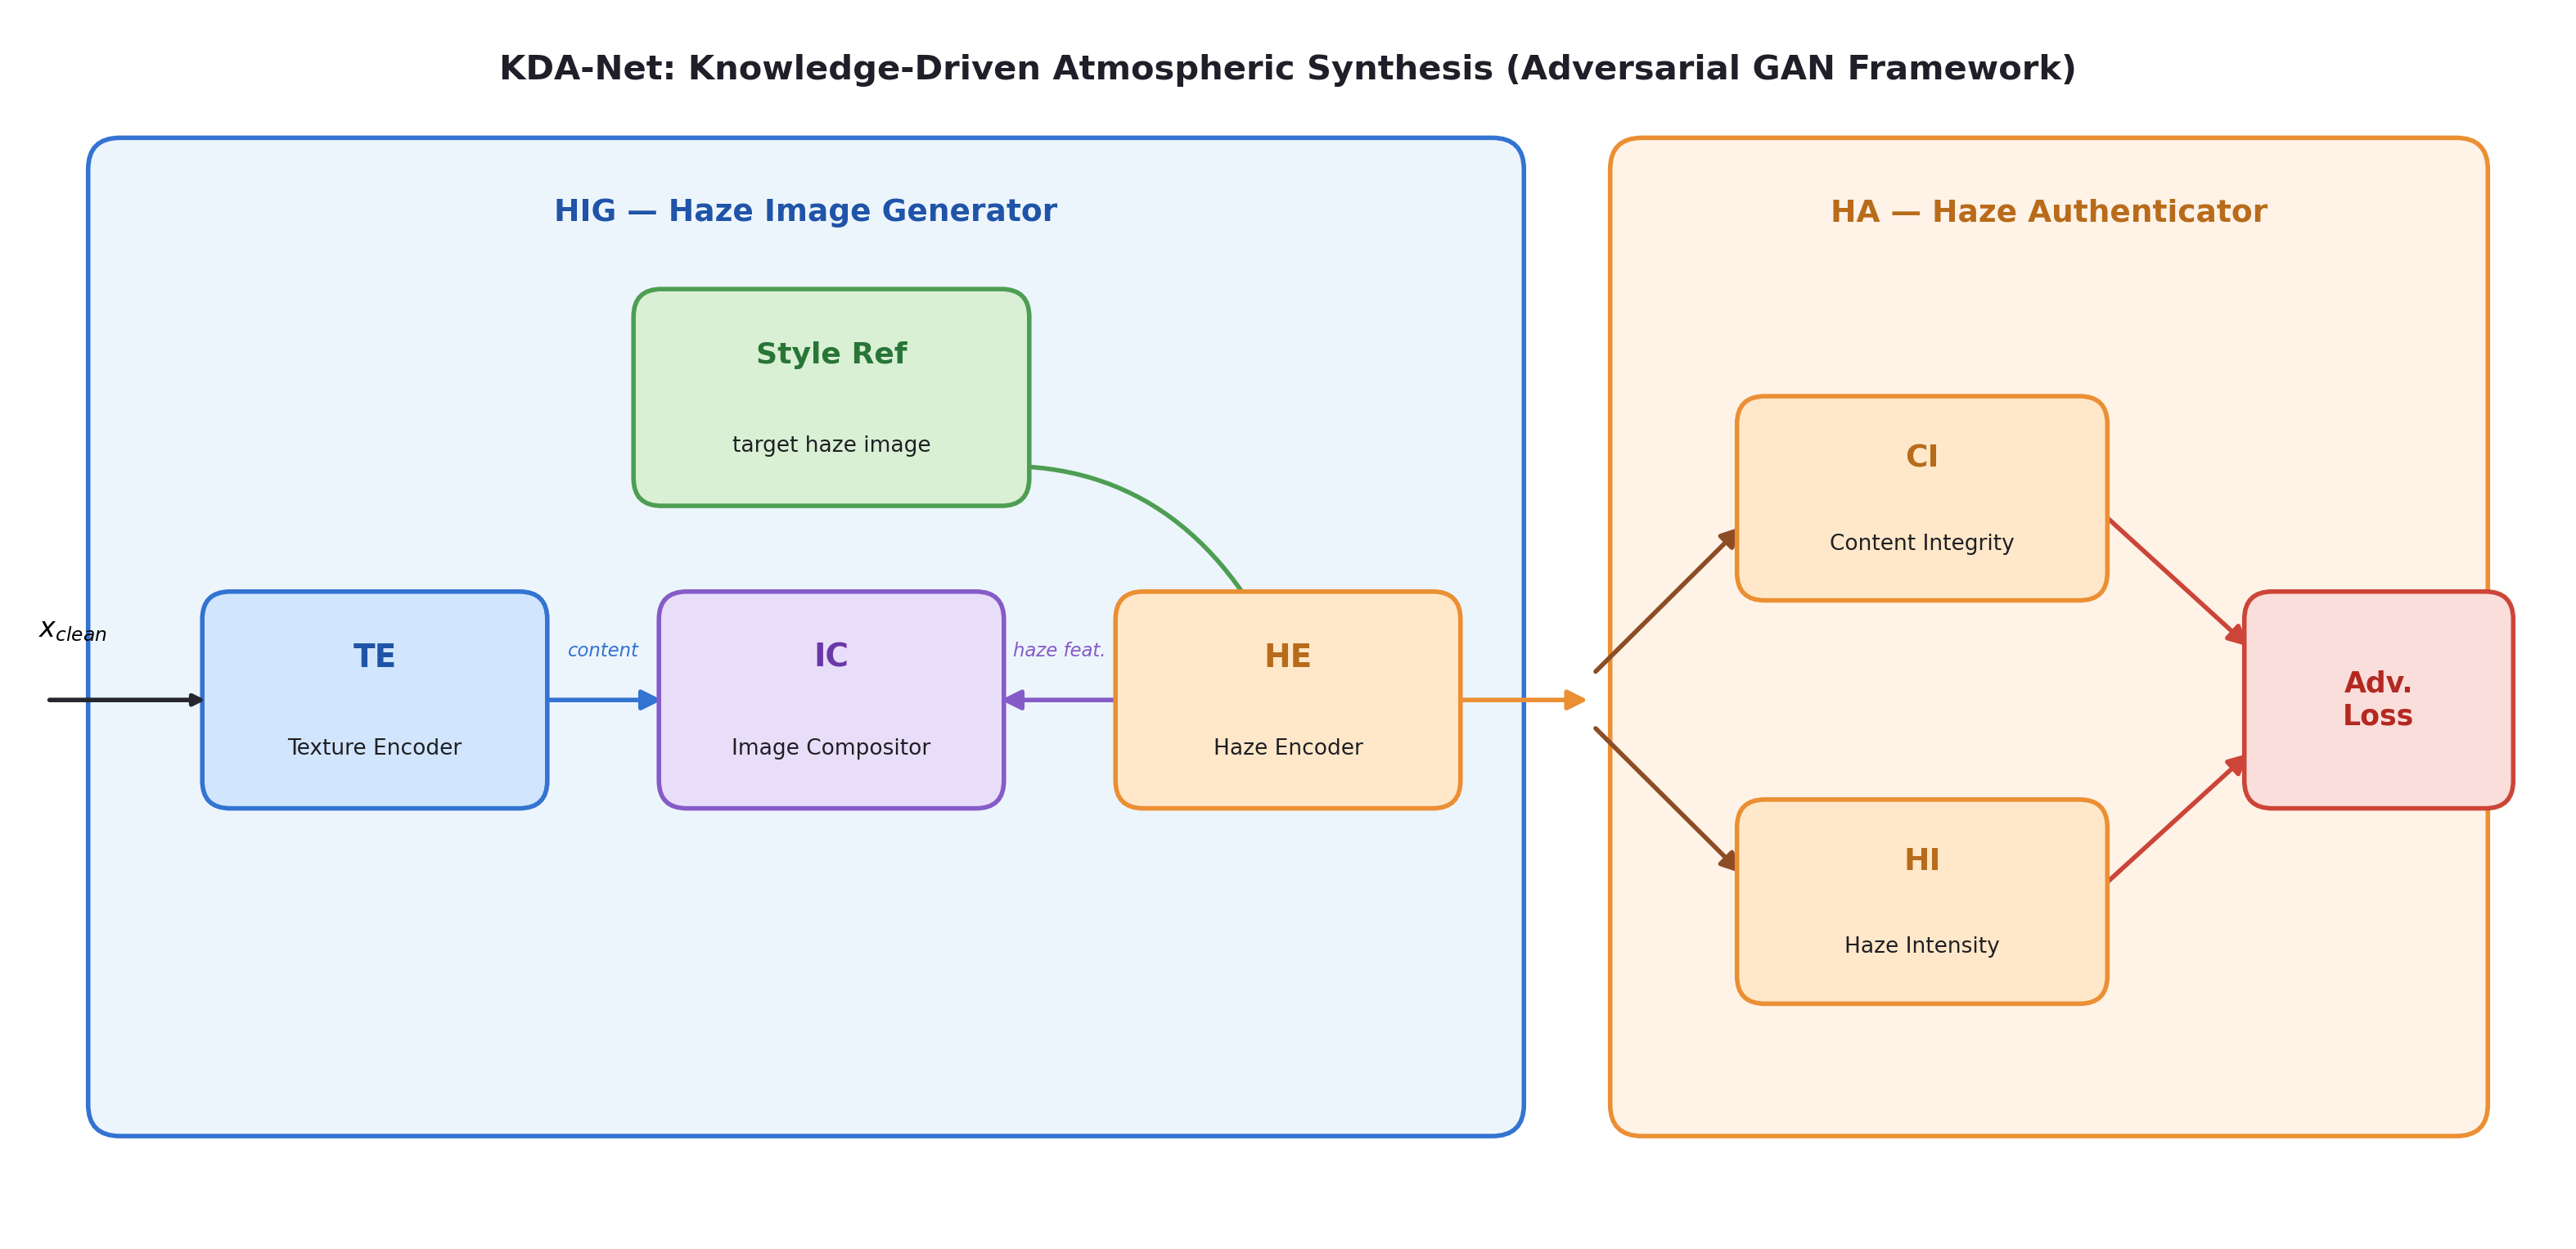
\includegraphics[width=0.97\linewidth]{images/kda_net_architecture.png}
    \caption{KDA-Net architecture: Haze Image Generator (HIG) with three modules (TE, HE, IC) and Haze Authenticator (HA) with two patch discriminators (CI, HI). The adversarial training was intended to enforce realism.}
    \label{fig:kda_net_architecture}
\end{figure}

\FloatBarrier
% -------------------------------------------------------
\subsection{Training and Failure}
\label{sec:kda_training}

\noindent KDA-Net was trained for 10--18 epochs without the GAN component (discriminators disabled) to first establish stable HIG outputs before introducing adversarial training. The non-adversarial training revealed a fundamental problem: the HIG converged to a solution with a persistent green colour cast across all outputs. The cause was traced to the IC module's learned blending weights, which systematically over-weighted the Haze Encoder features in the green channel. Without adversarial feedback from the HA to penalise this artefact, the HIG had no incentive to correct the colour distribution.

\noindent Attempts to fix the green cast through per-channel normalisation and colour loss terms were partially successful but did not eliminate it entirely. The adversarial training (re-enabled at epochs 15--18) was unstable: the CI discriminator collapsed early, and the HI discriminator overfit to the green cast rather than to genuine atmospheric texture. At 15:17 on June 5, 2025, the decision was made to restore the Koschmieder compositor as the Stage~3 standard and exclude KDA-Net outputs from all downstream experiments.

\noindent The KDA-Net architecture remains in the repository (\texttt{phase2\_pipeline/modules/kda\_net.py}) and the training code is intact. It represents a promising direction for future work: with a larger training dataset of real atmospheric images and extended adversarial training (50+ epochs), the colour cast could potentially be corrected and the learned compositor could surpass the simple Koschmieder model for complex atmospheric conditions.

\FloatBarrier
% =====================================================
\section{Complete Pipeline Parameter Tables}
\label{sec:pipeline_params}

\noindent Table~\ref{tab:v1_v2_v3_params} summarises all Stage~2 configuration parameters across V1--V4.

\begin{table}[htbp]
\centering
\caption{Complete parameter comparison across Stage~2 configurations V1--V4. V4 was discarded after qualitative inspection (see Section~\ref{sec:v4_discarded}); no quantitative metrics were collected.}
\label{tab:v1_v2_v3_params}
\renewcommand{\arraystretch}{1.3}
\resizebox{\textwidth}{!}{%
\begin{tabular}{lllll}
\toprule
\textbf{Parameter} & \textbf{V1} & \textbf{V2} & \textbf{V3} & \textbf{V4 (discarded)} \\
\midrule
IP-Adapter injection blocks & All (down+mid+up) & up\_blocks.0/1 only & up\_blocks.0/1 only & up\_blocks.0/1 only \\
IP-Adapter scale (haze) & 0.50 & 0.75 & 0.85 \\
IP-Adapter scale (sandstorm) & 0.50 & 0.78 & 0.88 \\
IP-Adapter scale (snow) & 0.50 & 0.72 & 0.82 \\
Img2img denoising strength & 0.60 & 0.62--0.70 & 0.72--0.74 & 0.72--0.74 \\
CSD guidance $\eta$ & 0.18 & 0.15--0.18 & None & 0.15 \\
CSD guidance interval & Every 3 steps & Every 3 steps & — & Every 3 steps \\
Koschmieder compositor & No & No & Yes & Yes \\
Text prompt & Detailed agricultural & Detailed agricultural & Minimal generic & Minimal generic \\
Spatial noise map & Yes ($s(x) = 0.55 + 0.20\,w_d$) & No & No & No \\
\midrule
ZS confidence (ViT-L-14) & 0.2978 & 0.3162 & 0.2740 & \textit{N/A (artefacts)} \\
Top-1 accuracy (ViT-L-14 / ViT-H-14) & — & 96.0\% / 95.3\% & 67.2\% / 67.4\% & \textit{N/A (artefacts)} \\
\bottomrule
\end{tabular}}
\end{table}


\FloatBarrier
% =====================================================
\section{Weather-Specific Physics Refinements}
\label{sec:weather_physics}

\noindent The V3 architecture established a stable foundation for atmospheric synthesis using the standard Koschmieder scattering model. However, further experimentation showed that some atmospheric phenomena require weather-specific physical modelling beyond a single extinction coefficient. Sandstorms are distinguished by large dust particles that scatter light differently across colour channels. Snowstorms add visible precipitation particles and surface accumulation that cannot be replicated by volumetric scattering alone.

\FloatBarrier
\subsection{V5: Sandstorm Wavelength-Dependent Scattering}
\label{sec:v5_sandstorm}

\noindent The classical Koschmieder model assumes a wavelength-independent extinction coefficient $\beta$. This assumption is sufficient for fog and haze, but does not reproduce the characteristic warm colour behaviour of sandstorms. Real sandstorms are dominated by mineral dust particles in the 1--100\,$\mu$m range, which scatter light in the Mie scattering regime. Unlike Rayleigh scattering (power-law exponent $\alpha \approx 4$, strongly wavelength-dependent), Mie scattering has $\alpha \approx 0.7$ — the attenuation varies only weakly with wavelength. However, even a small asymmetry across RGB channels is sufficient to produce the characteristic warm tint of airborne dust: blue is extinguished marginally faster than red, causing distant objects to shift toward amber-orange.

\noindent V5~(Table~\ref{tab:version_naming}) introduced channel-specific extinction coefficients calibrated to this regime:
\begin{equation}
    \beta_R = 0.87\,\beta, \qquad \beta_G = \beta, \qquad \beta_B = 1.15\,\beta.
\end{equation}

The full per-channel image formation model is applied independently for each colour channel $c \in \{R,G,B\}$:
\begin{equation}
    I_c(x) = J_c(x)\,e^{-\beta_c\,d(x)} + A_c\,\bigl(1 - e^{-\beta_c\,d(x)}\bigr),
\end{equation}
where $J_c(x)$ is the clean pixel value in channel $c$, $d(x)$ is the normalised scene depth from DPT-Large, and $A_c$ is the sandy atmospheric light colour ($A = [0.90,\,0.80,\,0.60]$ warm amber). Because $\beta_B > \beta_G > \beta_R$, the blue transmission decays fastest with depth. Distant objects progressively shift toward the sandy colour of the atmosphere; near objects retain their original colour. The result is a depth-consistent warm haze that cannot be reproduced by a single-channel compositor.

\begin{figure}[htbp]
    \centering
    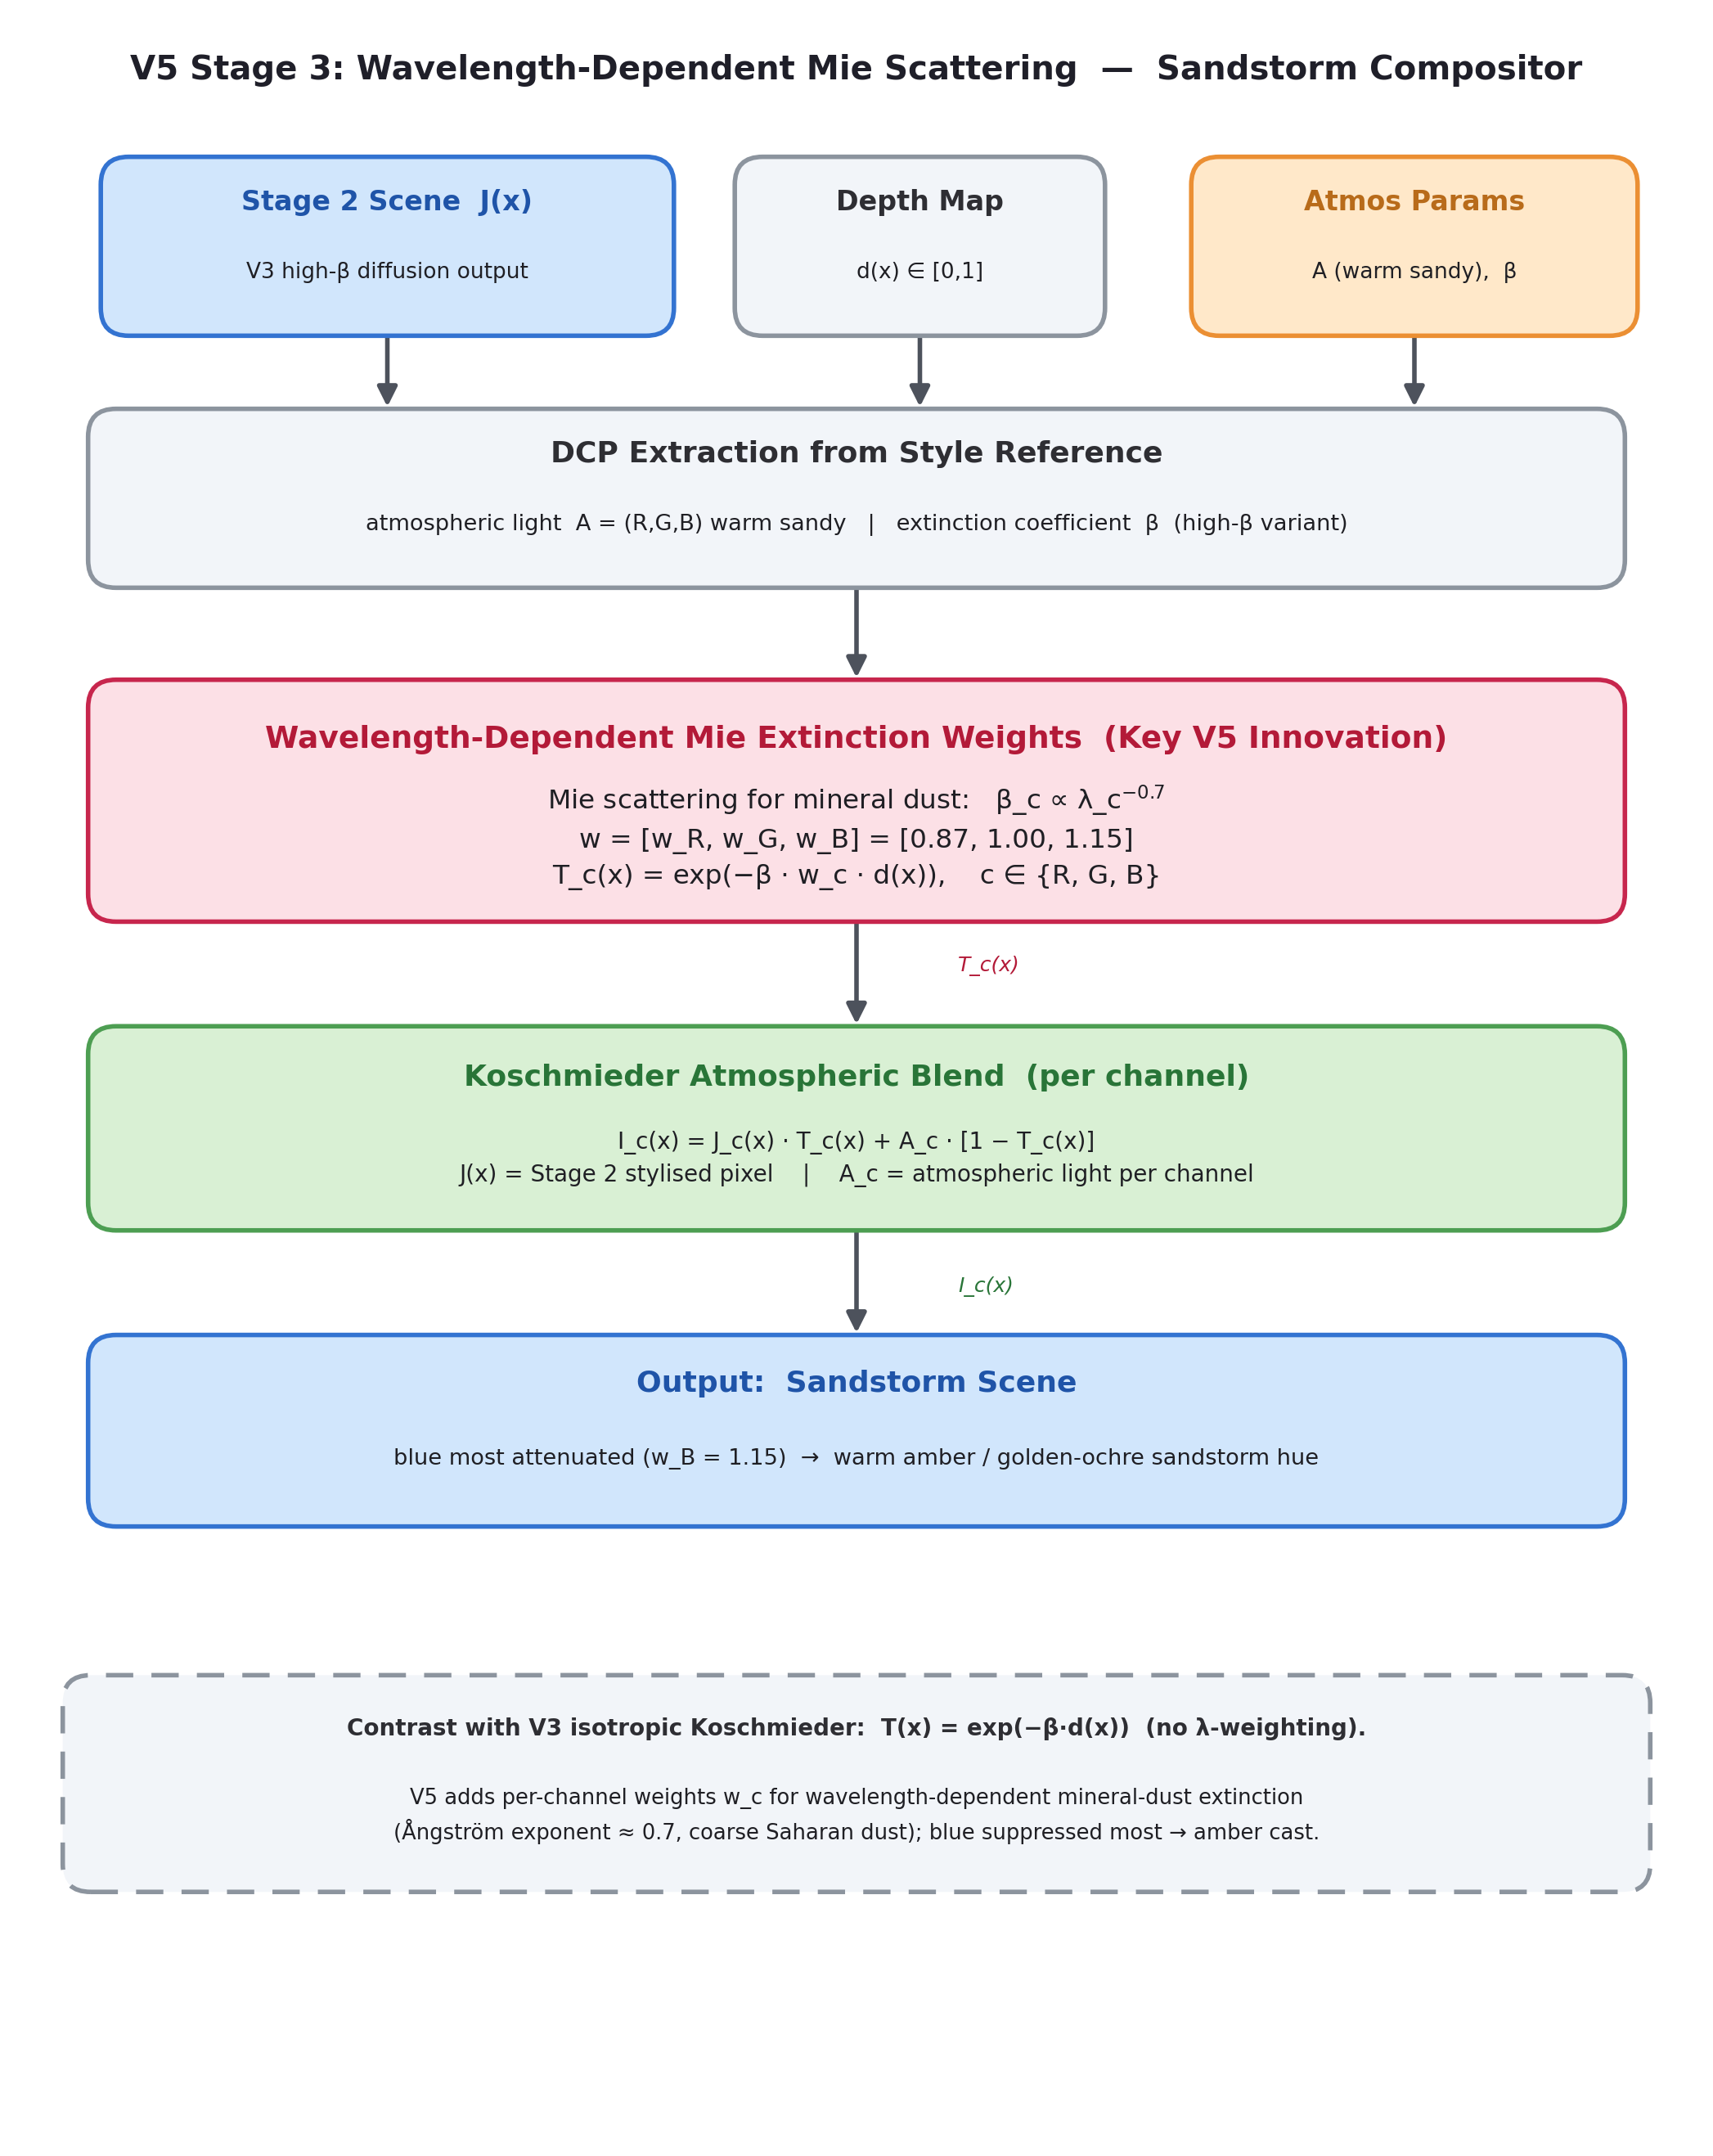
\includegraphics[width=0.82\linewidth]{images/arch_v5_stage3.png}
    \caption{V5 Stage~3 sandstorm compositor. The Stage~2 stylised scene, depth map, and DCP-extracted atmospheric parameters feed a wavelength-dependent Mie channel-weight block ($w_R{=}0.87$, $w_G{=}1.00$, $w_B{=}1.15$), yielding the warm amber sandstorm output. Per-channel equations are shown in the figure.}
    \label{fig:arch_v5_stage3}
\end{figure}

\begin{figure}[htbp]
    \centering
    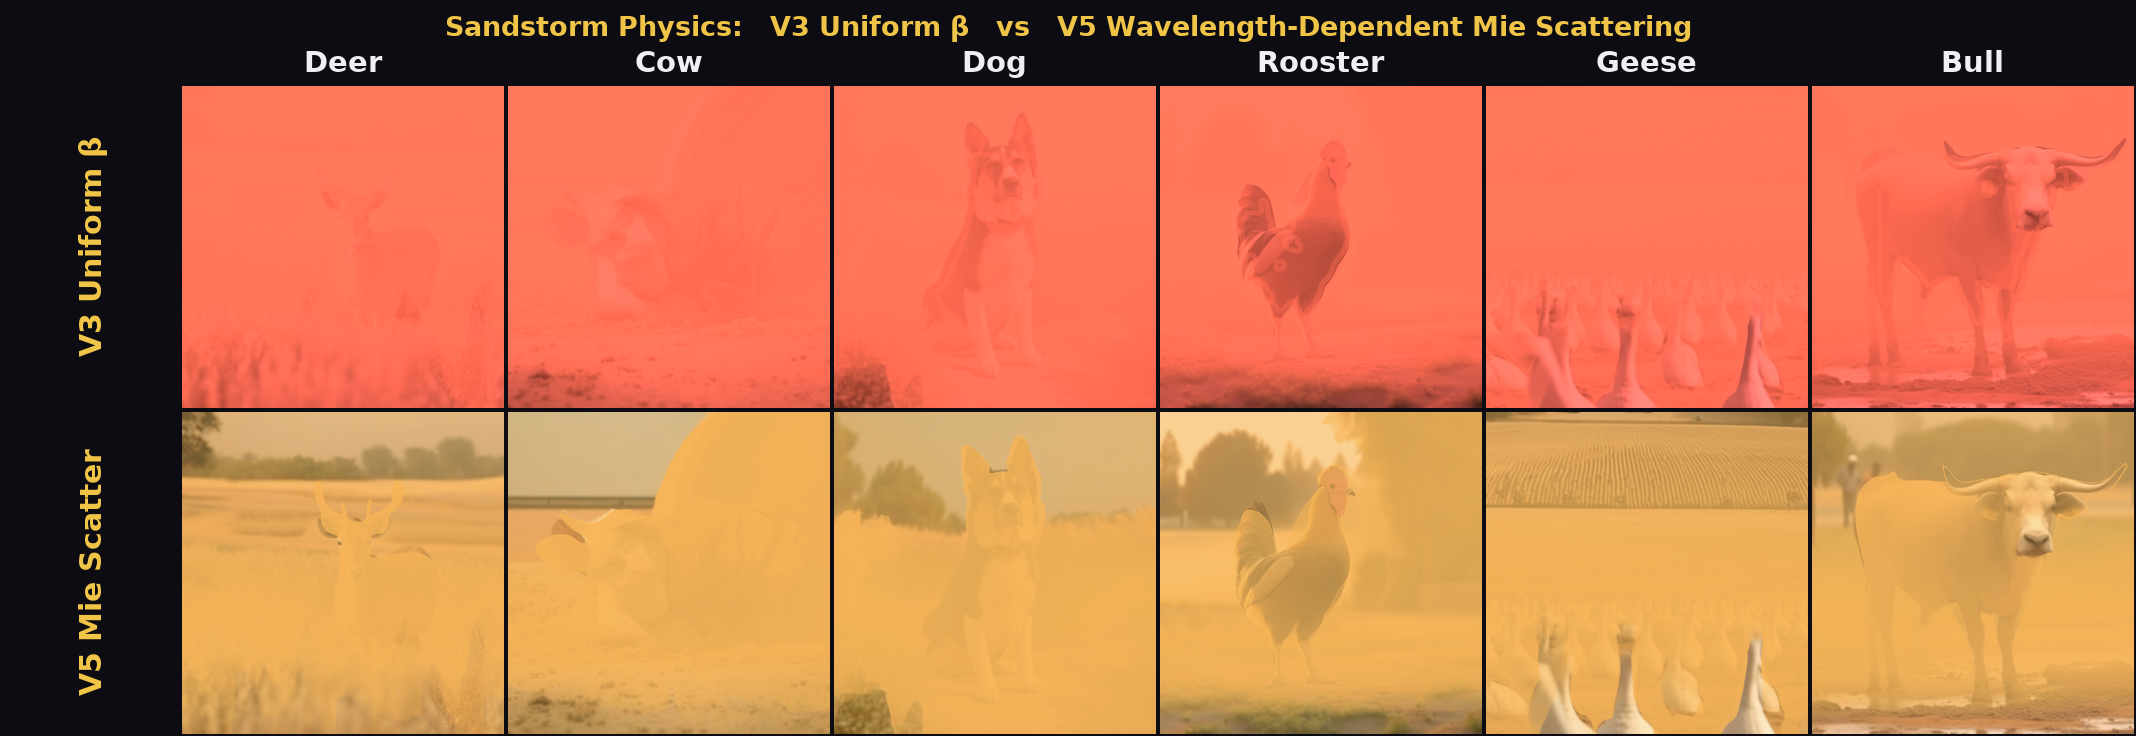
\includegraphics[width=0.96\linewidth]{images/v5_sandstorm.png}
    \caption{V3 uniform scattering vs.\ V5 wavelength-dependent Mie scattering applied to six content prompts (same sandstorm style reference). Channel-specific extinction coefficients ($\beta_B > \beta_G > \beta_R$) in V5 produce the characteristic warm amber colour shift of airborne mineral dust.}
    \label{fig:v5_sandstorm}
\end{figure}

\FloatBarrier
\subsection{V6: Procedural Snowfall Simulation}
\label{sec:v6_snowfall}

\noindent The key difference between snowstorms and fog or haze is that atmospheric particles are directly visible in the image. Individual snowflakes contribute to image formation and must be modelled separately from the volumetric scattering.

\noindent V6~(Table~\ref{tab:version_naming}) introduced a procedural snowfall layer computed after atmospheric compositing. Snow particles were generated using a depth-aware simulation where particle size, opacity, and blur radius vary according to estimated scene depth: larger particles appear closer to the camera; smaller, denser particles fill the far regions. Let $S(x)$ denote the synthesised snowfall layer. It is blended with the atmospheric image as:
\begin{equation}
    I_{\text{snow}}(x) = (1 - \alpha)\,I(x) + \alpha\,S(x),
\end{equation}
where $\alpha$ controls the snowfall intensity.

\noindent The visual result of V6~(Table~\ref{tab:version_naming}) snowfall is shown as the middle row of Figure~\ref{fig:v7_snow} alongside V3 and V7~(Table~\ref{tab:version_naming}) for direct comparison.

\FloatBarrier
\subsection{V7: Snow Accumulation Modelling}
\label{sec:v7_accumulation}

\noindent Although V6~(Table~\ref{tab:version_naming}) successfully generated snow particles, the images still lacked one of the most visually recognisable characteristics of snow environments: surface accumulation. Snow collects on horizontal surfaces — rooftops, farm equipment, fences, and ground regions — and this changes scene appearance in a way that cannot be replicated by atmospheric scattering or precipitation simulation alone.

\noindent V7~(Table~\ref{tab:version_naming}) applies three sequential stages to produce a physically complete winter scene.

\textbf{Stage 1 — Koschmieder base.} The standard depth-dependent compositor is applied with a cold white atmospheric light $A_{\text{snow}} = [0.92,\,0.94,\,0.98]$, causing distant objects to fade toward a blue-grey winter sky.

\textbf{Stage 2 — Surface accumulation.} A Sobel gradient computed on the DPT-Large depth map identifies locally flat regions. Surfaces with low gradient magnitude (flat), high nearness ($1-d(x)$), and upward-facing orientation (vertical weight) are assigned high accumulation probability. The accumulation mask $\alpha_g(x)$ is:
\begin{equation}
    \alpha_g(x) = \text{flatness}(x)\;\times\;\text{nearness}(x)\;\times\;\text{vertical\_weight}(x)\;\times\;\alpha_{\max},
\end{equation}
with $\alpha_{\max} = 0.70$. The accumulated image is then:
\begin{equation}
    I_a(x) = I_k(x)\,(1-\alpha_g(x)) + 255\cdot\alpha_g(x),
\end{equation}
where $I_k$ is the Koschmieder-composited image and the constant 255 represents the white snow colour.

\textbf{Stage 3 — Precipitation overlay.} Random snowflakes are placed at depth-weighted positions. Each flake has radius $r \in [1,\,4]$\,px and opacity $\alpha \in [0.25,\,0.90]$, both determined by nearness: foreground flakes are larger and more opaque; background flakes are smaller and translucent. The particle density is $\rho = 0.0008$ flakes per pixel. Let $M(x)$ denote the combined accumulation mask applied via Stage 2; the final output after all three stages is:
\begin{equation}
    I_{\text{accum}}(x) = (1 - M(x))\,I_{\text{snow}}(x) + M(x)\,C_{\text{snow}},
\end{equation}
where $I_{\text{snow}}$ includes the Stage 3 precipitation layer and $C_{\text{snow}}$ is the white snow colour. Only near, flat, and upward-facing surfaces accumulate snow; object boundaries and scene structure are preserved.

\begin{figure}[htbp]
    \centering
    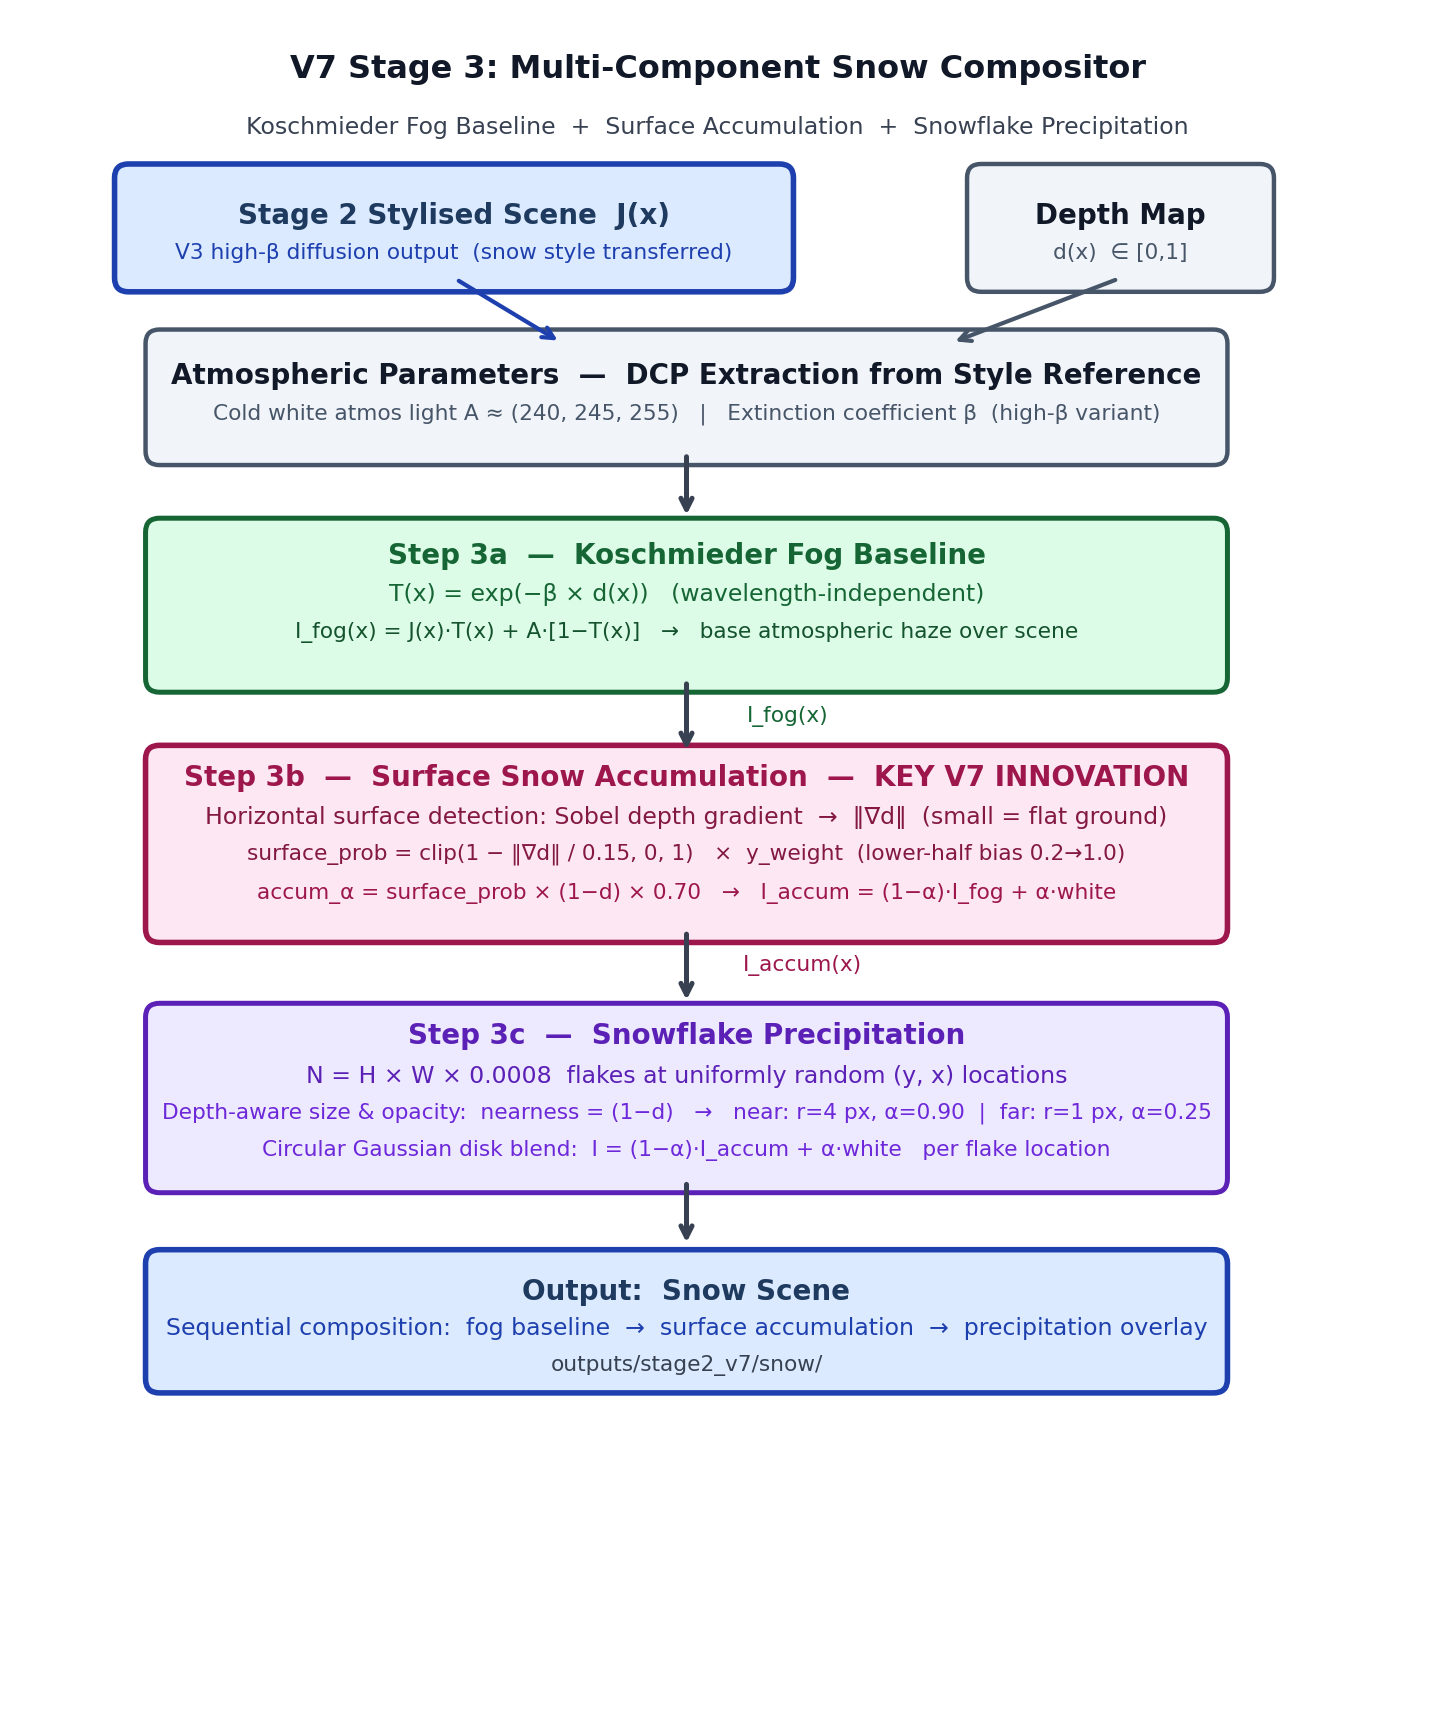
\includegraphics[width=0.82\linewidth]{images/arch_v7_stage3.png}
    \caption{V7 Stage~3 snow compositor architecture. The Stage~2 stylised scene and depth map feed through three sequential steps: \textbf{Step~3a} applies the standard Koschmieder fog baseline with cold white atmospheric light; \textbf{Step~3b} detects horizontal surfaces via Sobel depth gradients and overlays a white accumulation layer weighted by surface probability and nearness (max.\ opacity 0.70); \textbf{Step~3c} places $N = H \times W \times 0.0008$ snowflakes with depth-aware radius ($1$--$4$\,px) and opacity ($0.25$--$0.90$). The sequential composition produces a physically complete winter scene.}
    \label{fig:arch_v7_stage3}
\end{figure}

\begin{figure}[htbp]
    \centering
    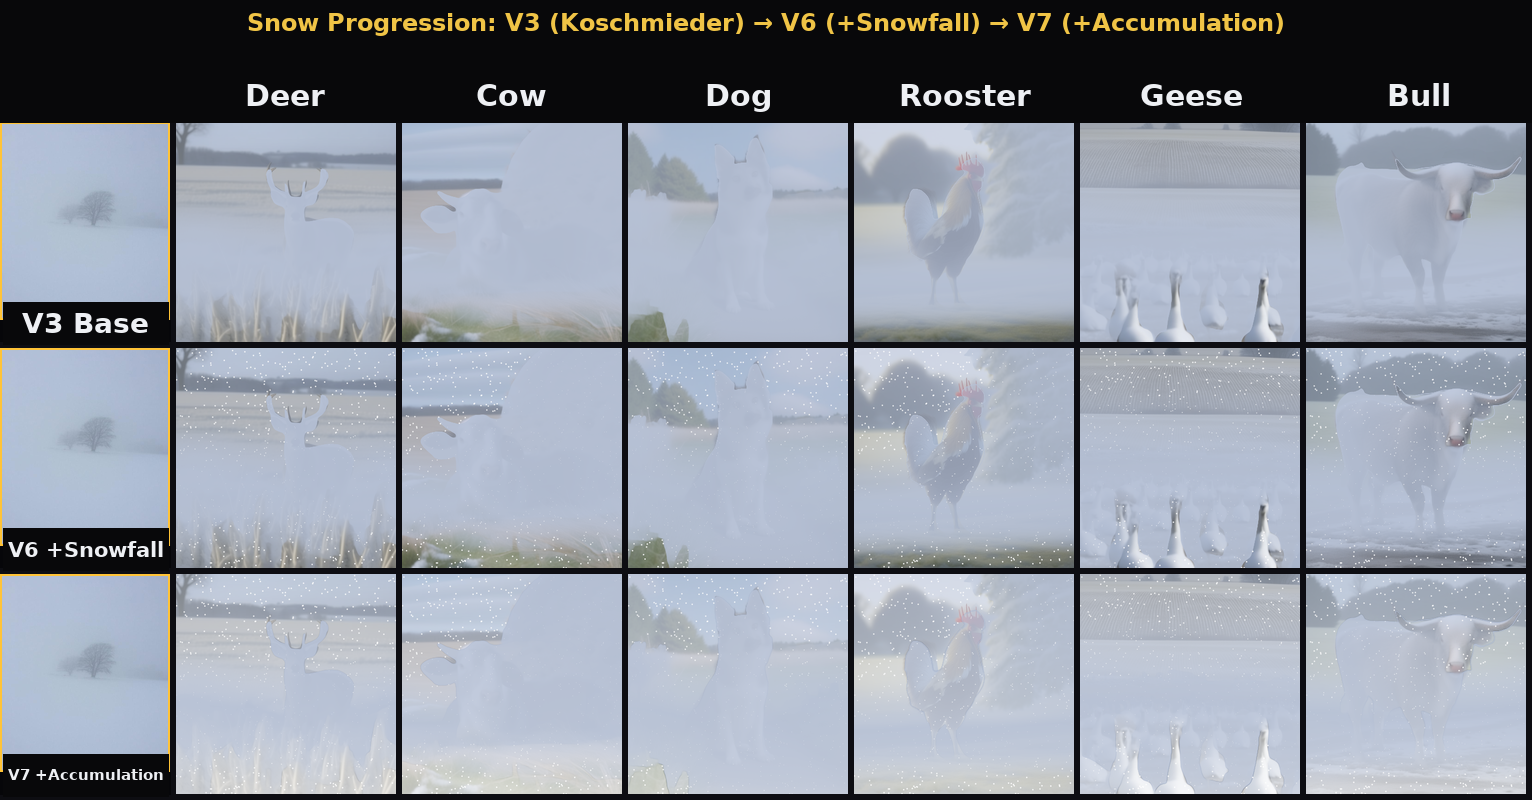
\includegraphics[width=0.96\linewidth]{images/v7_snow.png}
    \caption{Snow synthesis progression. V3~(top) applies Koschmieder visibility reduction; V6~(centre) adds depth-aware precipitation particles; V7~(bottom) further adds surface accumulation on plausible horizontal surfaces. V7 is the most physically complete winter model.}
    \label{fig:v7_snow}
\end{figure}

\begin{table}[htbp]
\centering
\caption{Summary of weather-specific physics refinements (V5--V7).}
\label{tab:physics_refinements}
\renewcommand{\arraystretch}{1.3}
\begin{tabular}{llp{7.5cm}}
\toprule
\textbf{Version} & \textbf{Focus} & \textbf{Core Contribution} \\
\midrule
V5 & Sandstorm Physics & Channel-specific Mie scattering ($\beta_B > \beta_G > \beta_R$) producing warm colour shift \\
V6 & Snowfall Simulation & Depth-aware procedural particle layer; foreground flakes larger than background \\
V7 & Snow Accumulation & Surface deposition mask from depth gradients; accumulation on horizontal surfaces \\
\bottomrule
\end{tabular}
\end{table}

\FloatBarrier
% -------------------------------------------------------
\section{V9: Content-Aware Atmospheric Style Transfer via Zero-Shot CLIP Embedding Subtraction}
\label{sec:v9}

\noindent V9~(Table~\ref{tab:version_naming}) addresses a fundamental limitation that persists across all prior configurations: \emph{content leakage from style reference images}. The style reference photographs used in Stages~V1--V3 are real-world atmospheric scenes that contain both the desired weather appearance (atmospheric texture, colour cast, visibility loss) and incidental semantic content (vegetation, ground plane, sky region, structures). The CLIP image encoder used by IP-Adapter captures both components simultaneously: the resulting image embedding is not a pure atmospheric descriptor but a superposition of atmospheric appearance and scene semantics. When this mixed embedding is injected into the SDXL generation process via IP-Adapter cross-attention, the content component contaminates the generated output — the synthesised scene inherits layout biases, vegetation density, and spatial arrangements from the style reference rather than from the content prompt.

\paragraph{Shared Embedding Space}
V9~(Table~\ref{tab:version_naming}) exploits a structural property of the SDXL and IP-Adapter architectures: the IP-Adapter image encoder (\texttt{CLIP ViT-bigG/14}) and the SDXL second text encoder (\texttt{text\_encoder\_2}) are initialised from the same \texttt{ViT-bigG/14} checkpoint and operate in the same 1280-dimensional embedding space. This co-residency is not coincidental — SDXL's dual-encoder design was specifically constructed so that the image-level CLIP representations and text-level CLIP representations are comparable within a shared geometric space~\cite{podell2023sdxlimprovinglatentdiffusion}. This property makes direct linear operations (summation, subtraction, interpolation) between image embeddings and text embeddings geometrically valid: the two modalities share the same basis directions, so subtracting a text direction from an image embedding removes the component of the image that aligns with the named concept.

\paragraph{Zero-Shot Content Identification}
The dominant semantic content of each style reference image is identified without any manual annotation. A candidate set $\mathcal{C}$ of 22 natural-language phrases is defined, covering common atmospheric scene subjects (persons, animals, vehicles, terrain, infrastructure). For a given style reference image $\mathbf{s}$, the dominant content label $c^*$ is determined by:
\begin{equation}
    c^* = \operatorname*{argmax}_{c \in \mathcal{C}} \; \cos\!\bigl(\phi_I(\mathbf{s}),\, \phi_T(c)\bigr),
    \label{eq:content_detection}
\end{equation}
where $\phi_I(\cdot)$ is the CLIP image encoder and $\phi_T(\cdot)$ is the CLIP text encoder. The candidate phrases include categories such as ``a person'', ``a tree'', ``farmland'', ``a road'', ``a mountain'', ``a building'', and additional domain-relevant terms. The highest-scoring candidate identifies the primary semantic object present in the style reference, requiring no labelled data or human supervision.

\paragraph{Content Subtraction in Embedding Space}
Given the detected content label $c^*$ and the original style reference embedding $\mathbf{e}_I = \phi_I(\mathbf{s})$, the content component is removed by projecting out the text direction $\mathbf{e}_T = \phi_T(c^*)$:
\begin{equation}
    \tilde{\mathbf{e}}_I = \mathrm{normalize}\!\Bigl(\hat{\mathbf{e}}_I - \alpha \cdot \hat{\mathbf{e}}_T\Bigr) \cdot \|\mathbf{e}_I\|,
    \label{eq:content_subtraction}
\end{equation}
where $\hat{\mathbf{e}}_I = \mathbf{e}_I / \|\mathbf{e}_I\|$ and $\hat{\mathbf{e}}_T = \mathbf{e}_T / \|\mathbf{e}_T\|$ are unit-normalised embeddings, $\alpha = 0.45$ is the subtraction strength, and the result is rescaled by the original norm $\|\mathbf{e}_I\|$ to preserve the magnitude expected by the IP-Adapter. The subtracted embedding $\tilde{\mathbf{e}}_I$ is used in place of $\mathbf{e}_I$ as the image prompt throughout Stage~2.

\noindent The operation in Equation~\ref{eq:content_subtraction} can be interpreted geometrically: the unit-normalised style embedding $\hat{\mathbf{e}}_I$ is shifted by $-\alpha \hat{\mathbf{e}}_T$ in the direction that would be activated by the concept $c^*$, followed by renormalisation to the unit hypersphere. The re-scaling by $\|\mathbf{e}_I\|$ preserves the injection intensity in IP-Adapter's cross-attention layers. This is analogous to concept vector arithmetic in distributed word embedding spaces, here applied to multimodal image–language embeddings.

\paragraph{Block Configuration and Inference Hyperparameters}
V9 adopts an extended block-selective injection scheme that includes the \texttt{mid\_block} in addition to the \texttt{up\_blocks.0} and \texttt{up\_blocks.1} blocks used in V3. The \texttt{mid\_block} operates at the bottleneck of the UNet and captures the highest-level structural features; including it improves low-frequency colour and luminance alignment with the atmospheric reference without the layout-leakage pathology of full all-block injection observed in V1. The IP-Adapter injection scale is set to 0.95 throughout. Unlike V3, V9 re-enables CSD guidance ($\eta=0.25$, $w_\mathrm{CSD}=1.5$, applied every 3 denoising steps using the raw style reference image $\mathbf{s}$); at the lower denoising strengths of pure t2i generation, CSD does not produce the destructive interference observed in V4 and instead provides complementary perceptual anchoring.

\begin{table}[htbp]
\centering
\caption{V9 configuration parameters.}
\label{tab:v9_config}
\begin{tabular}{ll}
\toprule
\textbf{Parameter} & \textbf{Value} \\
\midrule
Content detection candidates $|\mathcal{C}|$ & 23 \\
Content subtraction strength $\alpha$ & 0.45 \\
IP-Adapter injection blocks & \texttt{up\_blocks.0}, \texttt{up\_blocks.1}, \texttt{mid\_block} \\
IP-Adapter injection scale & 0.95 \\
Generation mode & Pure t2i (no img2img) \\
Denoising steps & 50 \\
Guidance scale & 7.5 \\
CSD guidance $\eta$ / weight / interval & 0.25 / 1.5 / every 3 steps \\
Style references per domain & 3 (haze, sandstorm, snow) \\
Random seeds per configuration & 3 \\
Stage~3 physics: haze & Koschmieder scattering (V3), $\beta_\mathrm{scale}=1.2$ \\
Stage~3 physics: sandstorm & Mie per-channel scattering (V5), $\mathbf{w}=[0.87,\,1.00,\,1.15]$ \\
Stage~3 physics: snow & Snowflake particles + surface accumulation (V7) \\
\bottomrule
\end{tabular}
\end{table}

\begin{figure}[htbp]
    \centering
    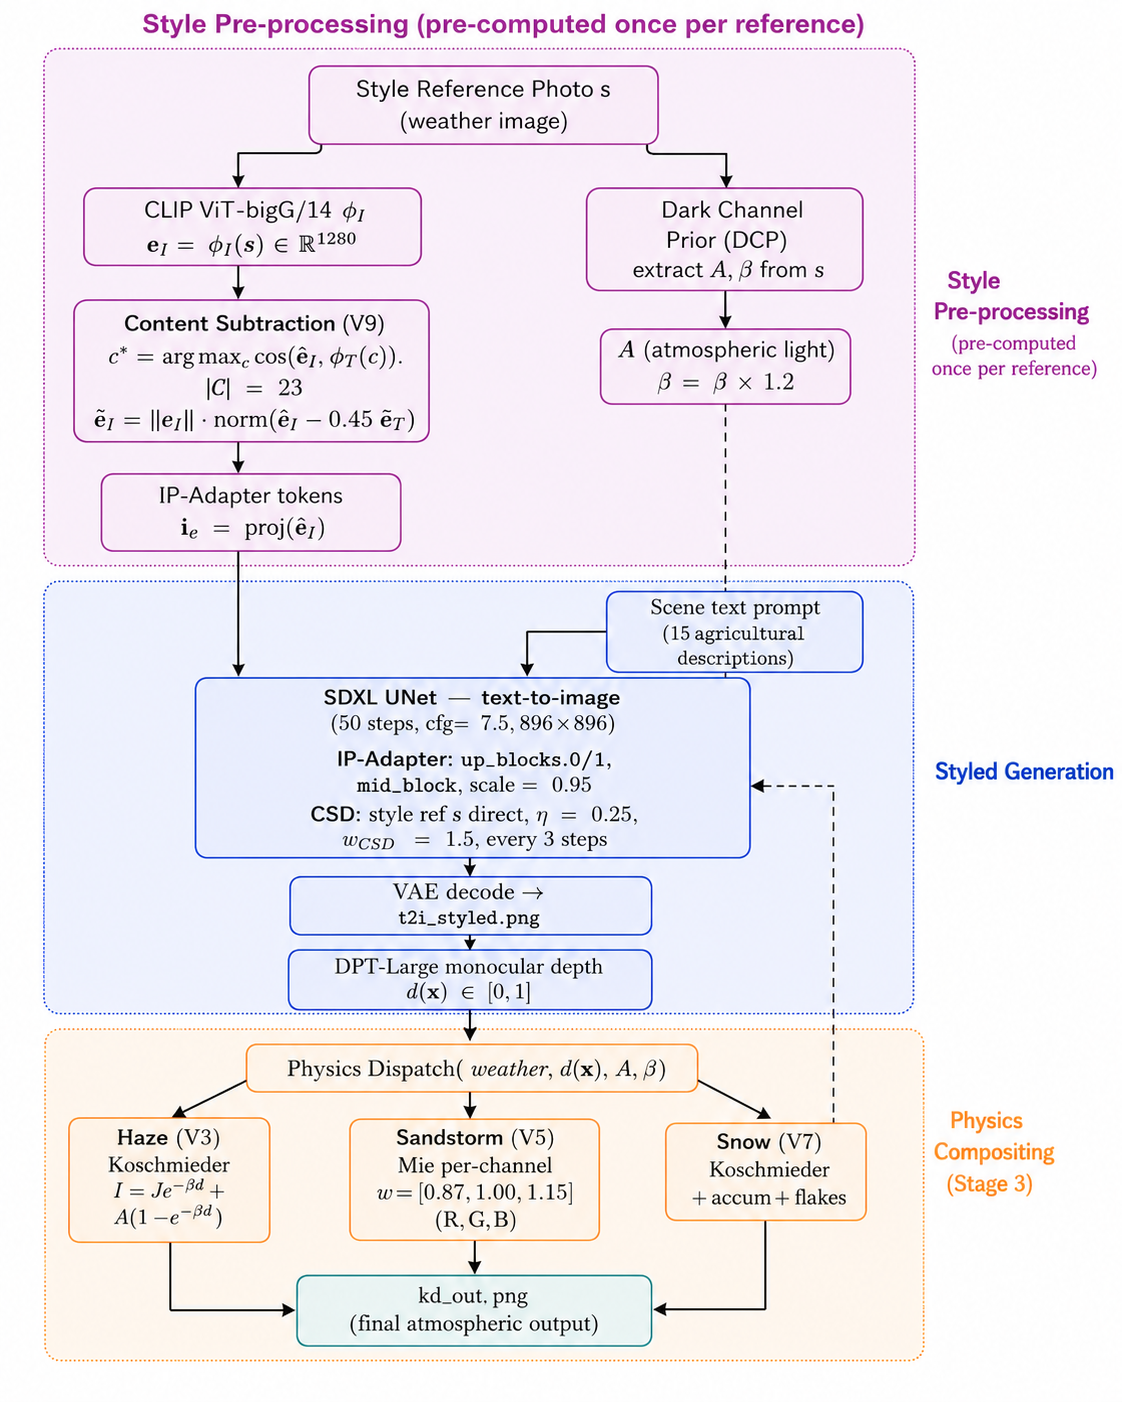
\includegraphics[width=0.95\linewidth, height=0.74\textheight, keepaspectratio]{images/v9_arch.png}
    \caption{V9 pipeline architecture. \textbf{Violet:} The style reference $\mathbf{s}$ is encoded by CLIP ViT-bigG/14; zero-shot content detection over 23 labels identifies $c^*$ whose text direction is subtracted ($\alpha=0.45$) to produce atmospheric-only IP tokens $\mathbf{ie}$. DCP extracts atmospheric light $A$ and extinction $\beta$ ($\times1.2$). \textbf{Blue:} Scene text prompt and $\mathbf{ie}$ drive SDXL t2i with block-selective IP-Adapter (\texttt{up$_0$/up$_1$/mid}, scale$=0.95$) and CSD ($\eta=0.25$, $w=1.5$, every 3 steps). \textbf{Orange:} DPT-Large depth and DCP-derived $A,\beta$ feed weather-specific physics: haze~(V3 Koschmieder), sandstorm~(V5 Mie per-channel), snow~(V7 + accumulation + snowflakes).}
    \label{fig:arch_v9_stage2}
\end{figure}

\paragraph{Weather-Specific Physics Dispatch}
The Stage~3 compositor in V9 dispatches to three physics backends depending on the atmospheric domain, rather than the single Koschmieder compositor used in V3:

\begin{itemize}
    \item \textbf{Haze}: Standard Koschmieder scattering (Equation~\ref{eq:koschmieder}) with scattering coefficients boosted by a scale factor $\beta_\mathrm{scale} = 1.2$ relative to DCP-estimated values, to produce denser and more visually challenging haze. Atmospheric light $A$ is estimated per-image from the style reference.
    \item \textbf{Sandstorm}: Mie scattering with per-channel attenuation weights $\mathbf{w} = [0.87,\, 1.00,\, 1.15]$ for the RGB channels respectively, reflecting the wavelength-dependent scattering of coarse mineral particulates under Mie theory (longer wavelengths scatter less, producing the characteristic warm amber-yellow tonal shift of sandstorm imagery).
    \item \textbf{Snow}: A two-component compositor comprising (i) simulated snowflake particle overlays (Gaussian blobs with randomised spatial placement at flake density $\rho_\mathrm{flake} = 8 \times 10^{-4}$ per pixel) and (ii) a surface accumulation layer applied to horizontal flat regions, with maximum accumulation opacity $\alpha_\mathrm{accum} = 0.70$.
\end{itemize}

\paragraph{Experimental Scale}
V9 was evaluated across 15 scene prompts $\times$ 9 style references (3 per atmospheric domain) $\times$ 3 random seeds, producing 405 images in total across the three atmospheric conditions. The complete set of 405 images was successfully generated, representing the final and most extensible configuration produced during this research.

\paragraph{Design Rationale and Limitations}
The fundamental design rationale of V9 is the separation of \emph{what the atmosphere looks like} (captured by the IP-Adapter style embedding) from \emph{what scene content is incidentally present} in the style reference (identified by zero-shot CLIP classification and removed by embedding subtraction). This disentanglement allows the generator to receive a more spectrally pure atmospheric signal during IP-Adapter injection. The approach requires no additional training, no labelled style reference annotations, and no modifications to the SDXL or IP-Adapter weights; the entire operation is performed at inference time on the pre-computed CLIP embeddings.

\noindent A practical limitation is that the subtraction strength $\alpha$ is a fixed scalar applied uniformly across all candidate–reference pairs. In style references where the dominant semantic content has a large projection onto the atmospheric signal (e.g., a hazy scene dominated by a single large tree that also provides the colour cast), setting $\alpha$ too high can inadvertently suppress genuine atmospheric components. The value $\alpha = 0.45$ was selected as a conservative balance point: sufficient to attenuate content interference without eliminating atmospheric colour and texture information.

\begin{figure}[H]
    \centering
    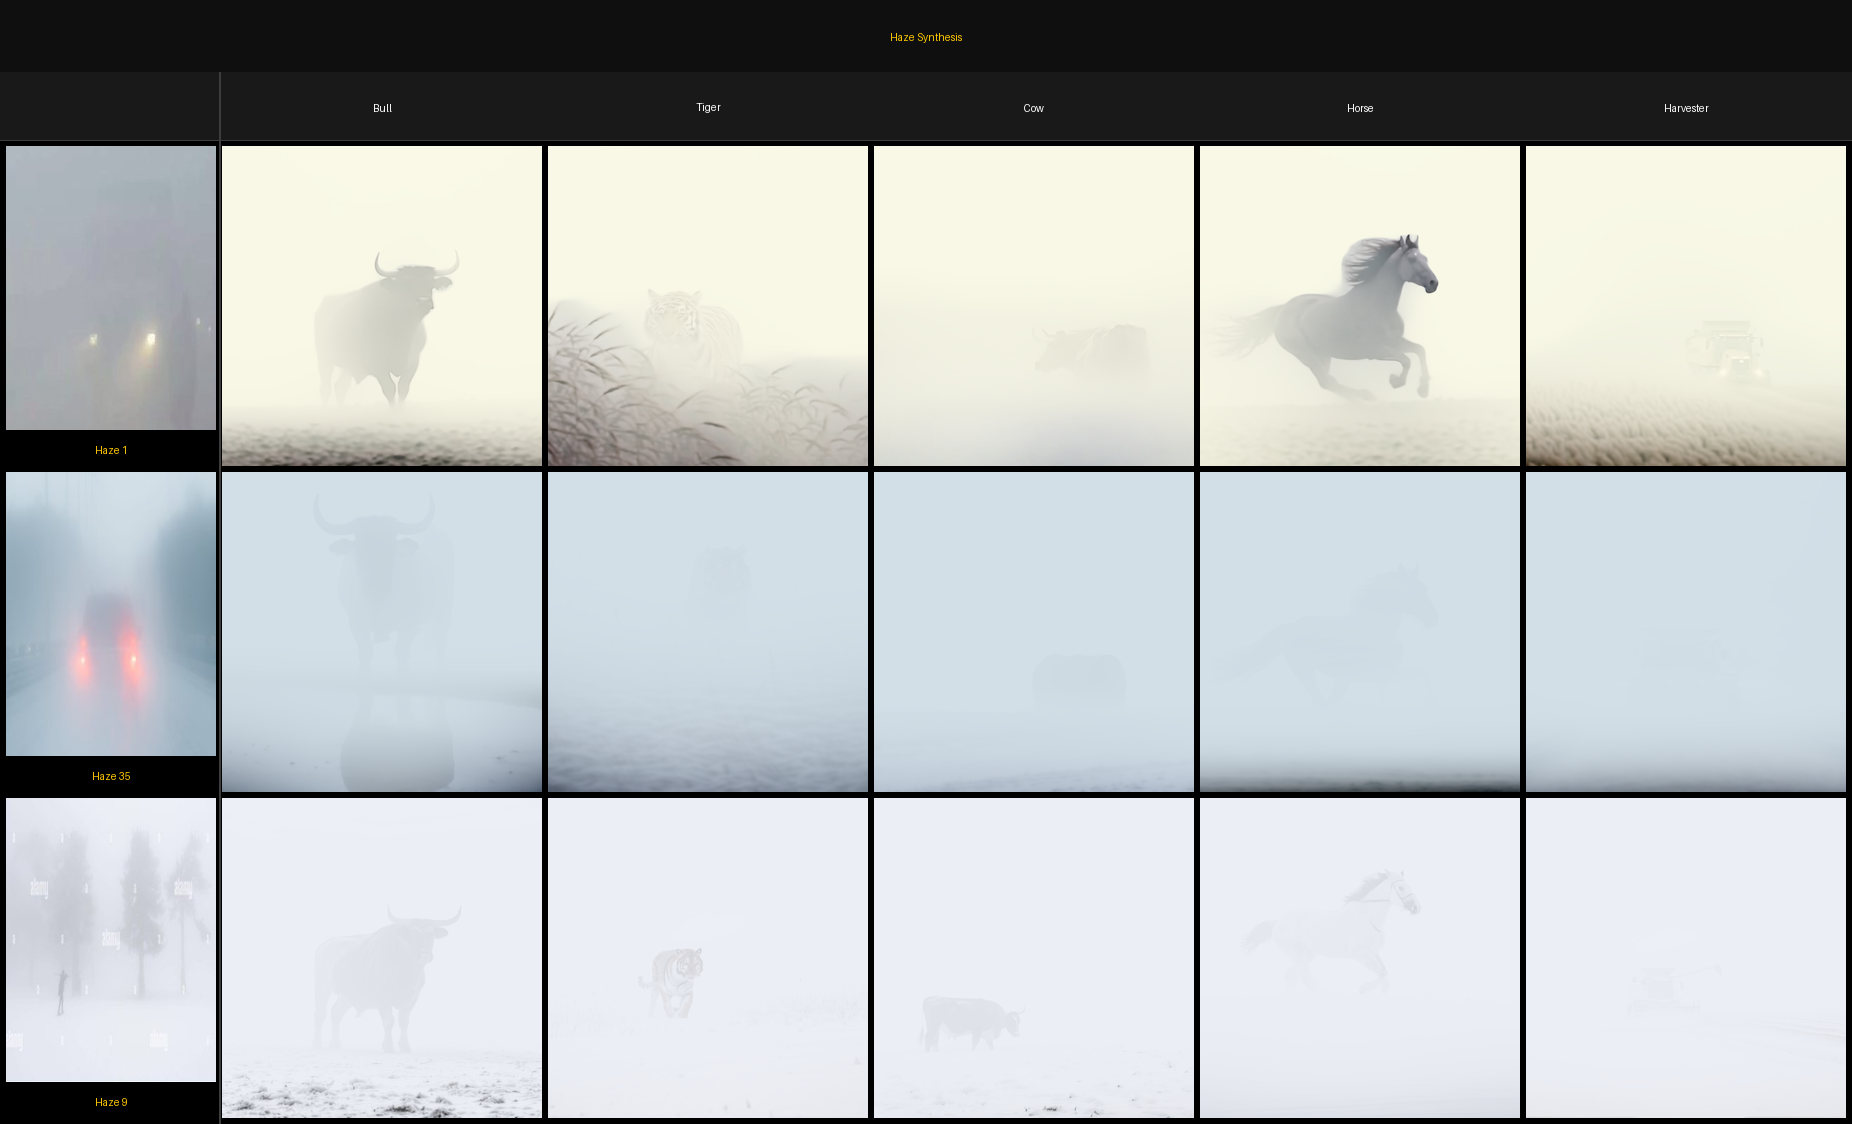
\includegraphics[width=0.96\linewidth]{images/haze_synthesis_v9.png}
    \caption{V9 haze synthesis results: three style references (rows) across five content subjects --- Bull, Tiger, Cow, Horse, and Harvester (columns). Each image is conditioned via CLIP content-subtraction ($\alpha = 0.45$) followed by Koschmieder physics compositing.}
    \label{fig:v9_haze_results}
\end{figure}

\begin{figure}[H]
    \centering
    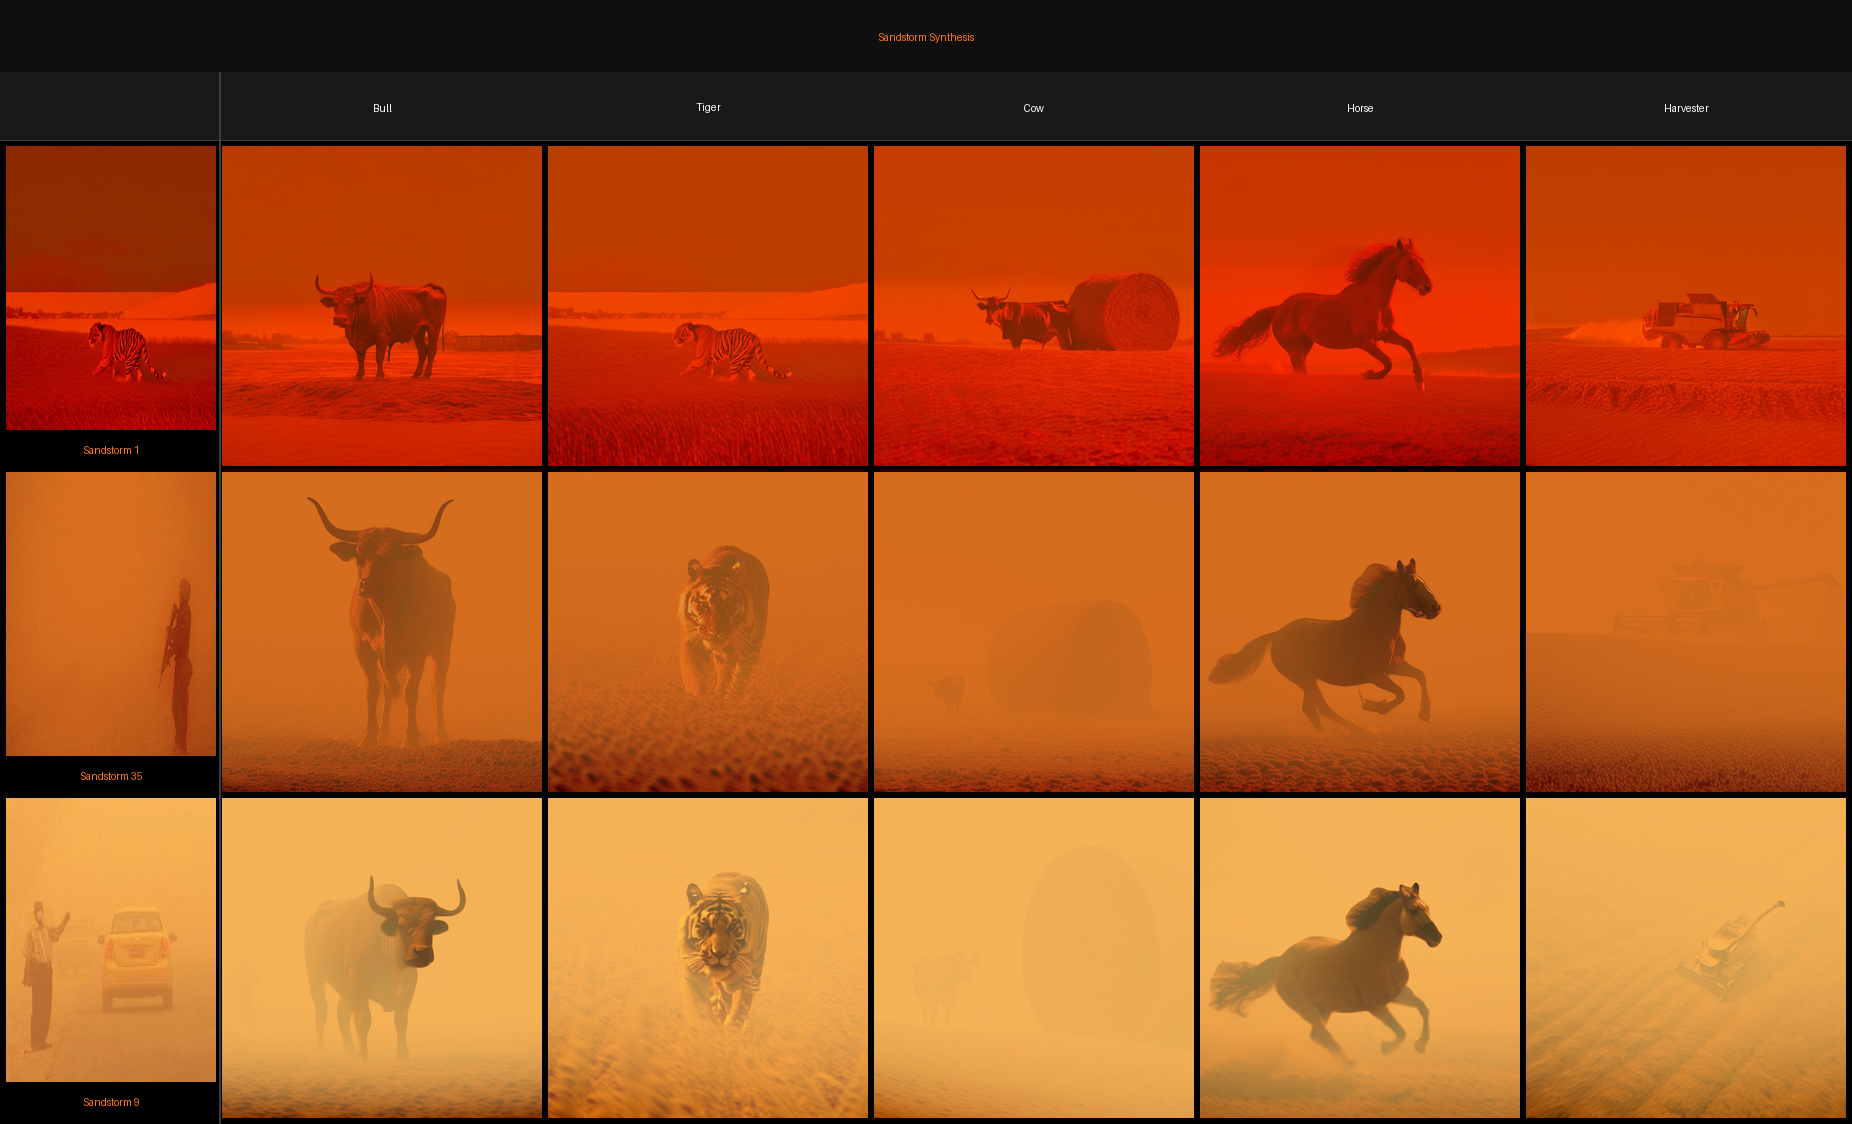
\includegraphics[width=0.96\linewidth]{images/sandstorm_synthesis_v9.png}
    \caption{V9 sandstorm synthesis results: three warm amber sand-dust style references (rows) across five content subjects (columns). Mie per-channel scattering ($\mathbf{w} = [0.87, 1.00, 1.15]$) in Stage~3 produces the characteristic warm amber tonal shift.}
    \label{fig:v9_sandstorm_results}
\end{figure}

\begin{figure}[H]
    \centering
    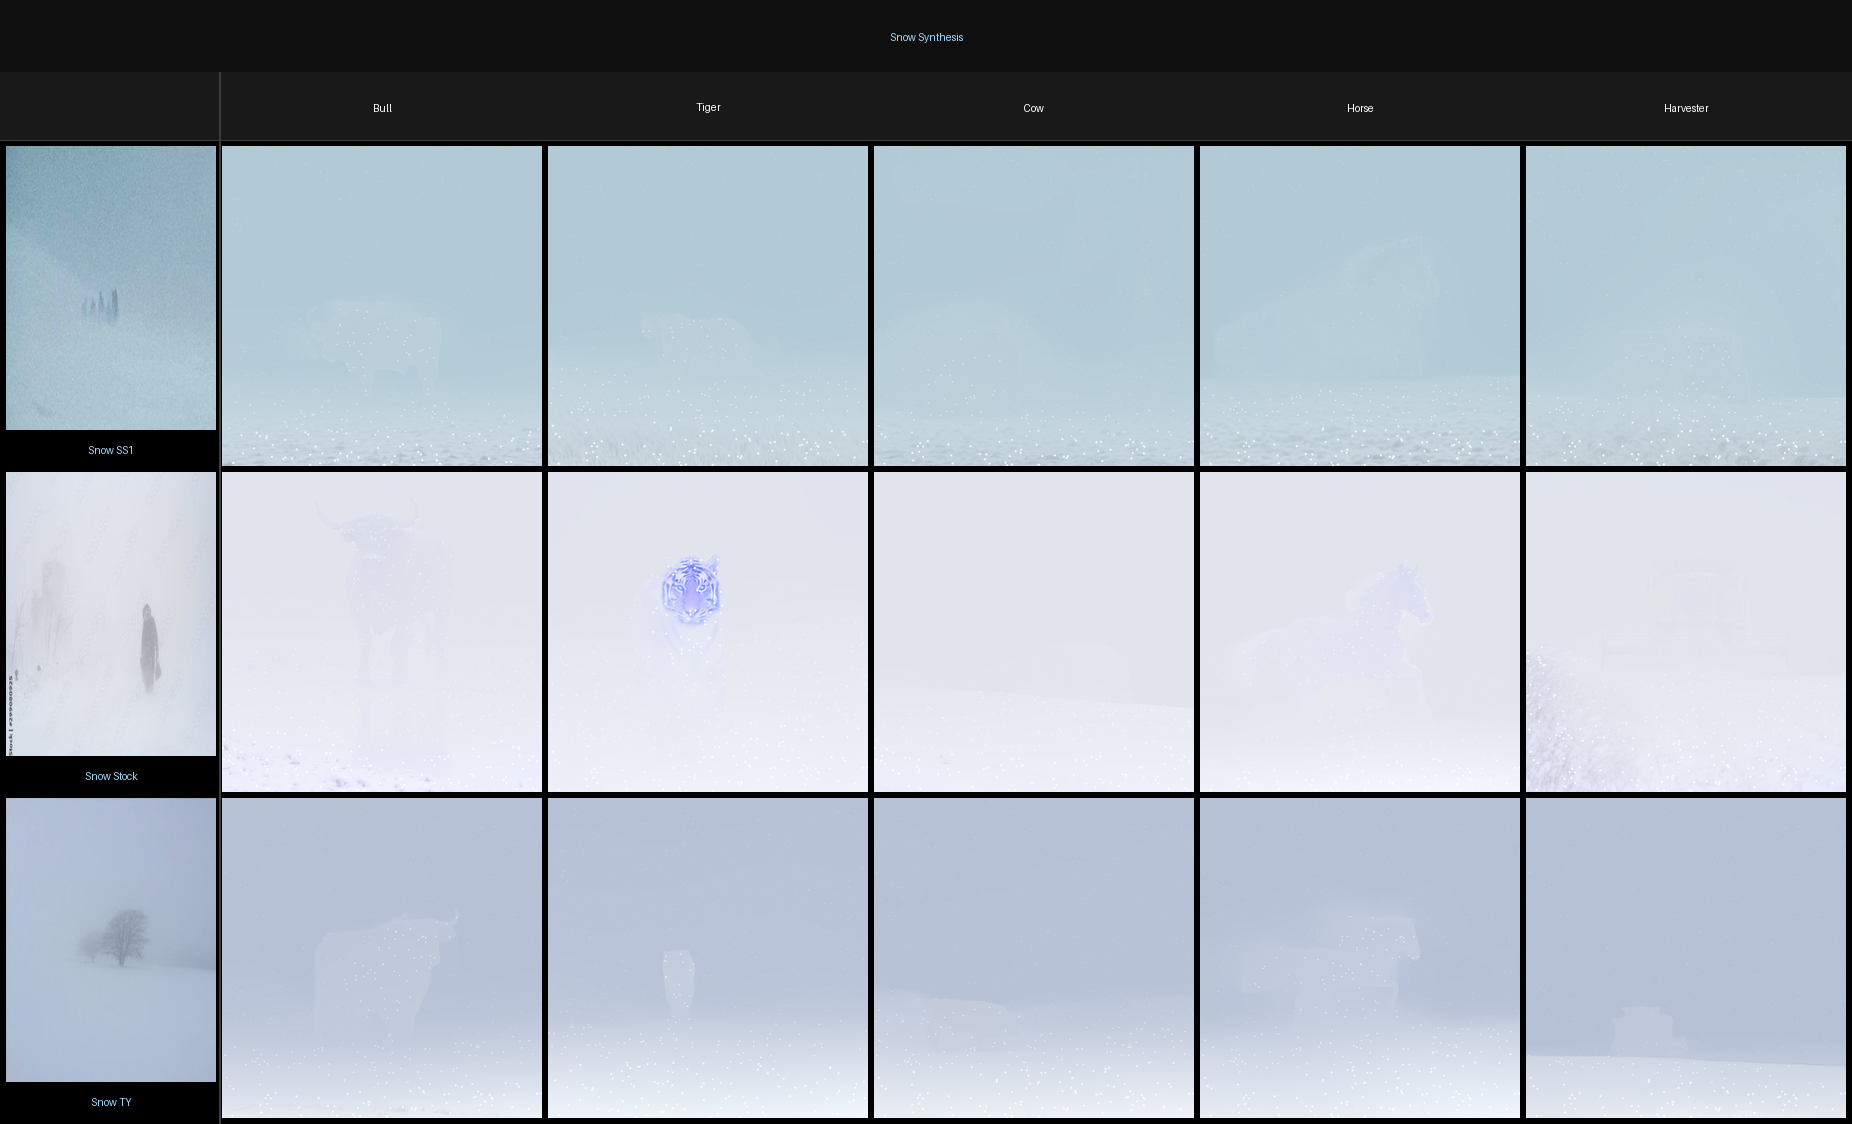
\includegraphics[width=0.96\linewidth]{images/snow_synthesis_v9.png}
    \caption{V9 snow synthesis results: three cold-weather style references (rows) across five content subjects --- Tiger, Deer, Dog, Boar, and Donkey (columns). Stage~3 adds snowflake particles and surface accumulation to achieve realistic winter scene compositing.}
    \label{fig:v9_snow_results}
\end{figure}

\FloatBarrier
% =====================================================
\section{Downstream Experiments}
\label{sec:phase2_experiments}

\noindent Five experiments were conducted using the synthesized atmospheric dataset to measure its utility for training vision models.

\paragraph{A Note on Metric Comparability with the Style Transfer Study}
Before presenting results, one potential source of confusion must be addressed. The style transfer study reported top-1 accuracy of \textbf{76.4\%} on style-transferred outputs while V3 of the proposed pipeline reports \textbf{67.2\%} on its outputs --- at first glance the proposed pipeline appears weaker on this metric. It is not.

The difference is entirely due to the classifier used. The most direct cross-method comparison uses a single metric: CLIP ViT-L-14 average max-softmax confidence. Lower confidence means the model is more uncertain about what class it is looking at, indicating stronger distributional shift. Table~\ref{tab:cross_phase_clip} shows the result.

\begin{table}[htbp]
\centering
\caption{Cross-method comparison on a unified metric: CLIP avg max-softmax confidence (lower = stronger domain shift = more physically realistic). All style transfer methods evaluated on the same agricultural content prompts used in the proposed pipeline (60 images per method, 4 atmospheric style references). Physics pipeline numbers from Experiment~1. Both ViT-L-14 and ViT-H-14 (metaclip\_fullcc) reported.}
\label{tab:cross_phase_clip}
\renewcommand{\arraystretch}{1.3}
\resizebox{\textwidth}{!}{%
\begin{tabular}{llcc}
\toprule
\textbf{Stage} & \textbf{Method / Split} & \textbf{ViT-L-14 Conf.\ ($\downarrow$)} & \textbf{ViT-H-14 Conf.\ ($\downarrow$)} \\
\midrule
Baseline          & Clean CIFAR-10              & 0.341 & 0.335 \\
\midrule
Style Transfer    & InstantStyle (baseline)     & 0.661 & 0.652 \\
Style Transfer    & InstantStyle-Plus           & 0.698 & 0.659 \\
Style Transfer    & StyleShot                   & 0.620 & 0.552 \\
Style Transfer    & CSGO                        & 0.625 & 0.587 \\
Style Transfer    & V0 (CSD-Guided Latent Optimisation) & 0.514 & 0.438 \\
\midrule
Physics Pipeline  & V2 (Block-Selective + CSD)                      & 0.316 & 0.303 \\
Physics Pipeline  & V3 (Physics-Grounded Atmospheric Compositing)   & 0.274 & 0.246 \\
Physics Pipeline  & V9 (Semantic-Decoupled Atmospheric Style Transfer) & \textbf{0.228} & \textbf{0.227} \\
\bottomrule
\end{tabular}}
\par\smallskip
{\footnotesize\noindent
V0 (IS+CSD Guidance) achieves the lowest confidence among all style transfer methods (0.514 / 0.438) but remains above the clean baseline (0.341 / 0.335) on both encoders. All physics pipeline methods fall below the clean baseline. \textbf{V9 achieves the lowest overall confidence (0.228 / 0.227) of any method evaluated}, representing the strongest domain shift.}
\end{table}

\noindent A controlled re-evaluation on the same 15 agricultural prompts and 4 atmospheric style references reveals a clear three-level hierarchy. The four passive style transfer baselines (InstantStyle, InstantStyle-Plus, StyleShot, CSGO) yield CLIP ViT-L-14 confidence between 0.620 and 0.698 --- well above both the ViT-L-14 clean baseline (0.341) and the ViT-H-14 clean baseline (0.335), indicating that passive style injection does not substantially confuse modern vision encoders. V0~(Table~\ref{tab:version_naming}) (InstantStyle + CSD Guidance), with active latent correction, reduces confidence to 0.514 (L-14) and 0.438 (H-14) --- the lowest of any style transfer method --- yet both values remain above the clean baseline (0.341 / 0.335), confirming that appearance-based style injection cannot cross this threshold regardless of guidance sophistication. V3 at 0.274 (L-14) / 0.246 (H-14) falls below both clean baselines, and \textbf{V9 achieves the strongest domain shift of all evaluated methods (0.228 / 0.227)}, demonstrating that zero-shot CLIP content subtraction combined with physics compositing produces a fundamentally deeper distributional shift than anything achievable with learned style transfer alone.

% -------------------------------------------------------
\FloatBarrier
\subsection{Experiment 1: Pipeline Comparison (V3 vs V9)}
\label{sec:exp1}

\noindent \textbf{Goal:} Determine whether V9's zero-shot CLIP content subtraction and extended block injection produce a stronger feature-space domain shift than the V3 baseline across all three atmospheric conditions.

\noindent \textbf{Data.} Both pipelines produce 405 images each (15 prompts $\times$ 9 style references $\times$ 3 seeds, across haze, sandstorm, and snow). The same ViT-L-14 and ViT-H-14 (metaclip\_fullcc) encoders are used throughout, with mean max cosine-softmax confidence over a 100-class ImageNet vocabulary as the primary metric.

\begin{table}[htbp]
\centering
\caption{Experiment~1: Zero-shot confidence and Top-1 accuracy on V3 and V9 pipeline outputs. Lower confidence = stronger domain shift. Per-weather breakdown shows where each pipeline's atmospheric effect is strongest.}
\label{tab:exp1_pipeline_comparison}
\renewcommand{\arraystretch}{1.3}
\resizebox{\textwidth}{!}{%
\begin{tabular}{llcccc}
\toprule
\textbf{Pipeline} & \textbf{Weather} & \multicolumn{2}{c}{\textbf{ZS Confidence ($\downarrow$)}} & \multicolumn{2}{c}{\textbf{Top-1 Accuracy ($\downarrow$)}} \\
\cmidrule(lr){3-4}\cmidrule(lr){5-6}
& & \textbf{ViT-L-14} & \textbf{ViT-H-14} & \textbf{ViT-L-14 (\%)} & \textbf{ViT-H-14 (\%)} \\
\midrule
Clean scenes & All & 0.339 & 0.334 & — & — \\
\midrule
\multirow{4}{*}{V3} & Haze       & \textbf{0.219} & \textbf{0.220} & 60.7 & 60.7 \\
                    & Sandstorm  & 0.302          & 0.266          & 68.9 & 68.2 \\
                    & Snow       & 0.289          & 0.267          & 70.4 & 73.3 \\
                    & \textit{All} & 0.270        & 0.249          & 68.4 & 67.2 \\
\midrule
\multirow{4}{*}{V9} & Haze       & 0.231          & 0.244          & 62.2 & 61.5 \\
                    & Sandstorm  & 0.281          & 0.261          & 78.5 & 80.0 \\
                    & Snow       & \textbf{0.171} & \textbf{0.180} & \textbf{41.5} & \textbf{37.8} \\
                    & \textit{All} & \textbf{0.228} & \textbf{0.227} & \textbf{62.2} & \textbf{59.8} \\
\bottomrule
\end{tabular}}
\end{table}

\noindent V9 achieves the lowest overall confidence on both backbones (0.228 vs 0.270 for ViT-L-14; 0.227 vs 0.249 for ViT-H-14). The per-weather breakdown reveals a clear pattern: V3 haze is marginally stronger (0.219 vs 0.231), but V9 snow is dramatically more challenging — 0.171 ViT-L-14, the lowest single-condition score in the entire study. This is a direct consequence of V7~(Table~\ref{tab:version_naming})'s two-component snow compositor (surface accumulation + precipitation particles), which alters scene appearance more aggressively than any pure visibility-based model. V9 sandstorm also slightly outperforms V3 (0.281 vs 0.302), attributable to V5~(Table~\ref{tab:version_naming})'s wavelength-dependent Mie scattering preserving the warm colour cast at greater depth.

\noindent The corresponding Top-1 accuracy drop is most striking for snow: from 70.4\% (V3) to 41.5\% (V9) on ViT-L-14. This means that for nearly 60\% of V9 snow images, the pretrained ViT cannot confidently identify the correct agricultural scene class — confirming that the V9 snow model produces a qualitatively harder recognition problem than any prior pipeline version.

% -------------------------------------------------------
\FloatBarrier
\subsection{Experiment 2: Linear Probe Adaptation}
\label{sec:exp2}

\noindent \textbf{Goal:} Measure how much of the atmospheric domain gap can be closed by linear probing on frozen ViT features, and whether a probe trained on V3 data transfers to V9 images — and vice versa.

\noindent \textbf{Setup.} Two separate linear probes are trained: one on V3 highbeta (405 images, 80/20 split) and one on V9 (405 images, 80/20 split). Both use \texttt{LogisticRegression} on L2-normalised CLIP image features with no backbone fine-tuning. Cross-distribution evaluation tests whether the V3-trained probe transfers to V9 images without retraining.

\begin{table}[htbp]
\centering
\caption{Experiment~2: Zero-shot vs linear probe accuracy across evaluation sets. V3 and V9 probes work in-distribution but do not cross-transfer, confirming that each physics pipeline creates a distinct feature-space distribution.}
\label{tab:exp2_linear_probe}
\renewcommand{\arraystretch}{1.3}
\resizebox{\textwidth}{!}{%
\begin{tabular}{llccc}
\toprule
\textbf{Backbone} & \textbf{Eval Set} & \textbf{Zero-Shot} & \textbf{Linear Probe} & \textbf{Gain} \\
\midrule
\multirow{4}{*}{ViT-L-14}
  & V3 test split (in-dist)        & 79.0\% & 86.4\% (V3 probe)  & +7.4 pp \\
  & Extreme haze ($\beta=9.0$)     & 82.2\% & 93.3\% (V3 probe)  & +11.1 pp \\
  & V9 test split (in-dist)        & 66.7\% & 76.5\% (V9 probe)  & +9.8 pp \\
  & V9 images (V3 probe xfer)      & 65.9\% & 65.4\% (V3 probe)  & $-$0.5 pp \\
\midrule
\multirow{4}{*}{ViT-H-14}
  & V3 test split (in-dist)        & 77.8\% & 87.7\% (V3 probe)  & +9.9 pp \\
  & Extreme haze ($\beta=9.0$)     & 86.7\% & 93.3\% (V3 probe)  & +6.6 pp \\
  & V9 test split (in-dist)        & 65.4\% & 71.6\% (V9 probe)  & +6.2 pp \\
  & V9 images (V3 probe xfer)      & 65.7\% & 60.2\% (V3 probe)  & $-$5.5 pp \\
\bottomrule
\end{tabular}}
\end{table}

\noindent Two findings stand out. First, both probes produce meaningful in-distribution gains: the V3 probe achieves +7.4 pp (ViT-L-14) on V3 test data, and the V9 probe achieves +9.8 pp on V9 test data. The V3 probe also generalises well to extreme synthetic haze ($\beta = 9.0$, 3$\times$ normal density), confirming that the probe has learned to handle atmospheric degradation within the same physics regime.

\noindent Second, \textbf{cross-distribution transfer completely fails}: the V3-trained probe applied to V9 images yields $-$0.5 pp and $-$5.5 pp relative to zero-shot on ViT-L-14 and ViT-H-14 respectively — essentially no improvement or a regression. This is a direct consequence of V9's CLIP content subtraction and extended block injection fundamentally altering the feature-space distribution relative to V3. A probe adapted to V3's IP-Adapter style transfer characteristics does not transfer to V9's content-subtracted embeddings, even though both datasets cover the same 15 scene classes. Each pipeline version requires its own domain adaptation.

% -------------------------------------------------------
\FloatBarrier
\subsection{Experiment 3: Probe Generalisation to Real Animal Photographs}
\label{sec:exp3}

\noindent \textbf{Goal:} Test whether probes trained entirely on \emph{synthetic} atmospheric images (V3 or V9) generalise to recognise \emph{real} animal photographs that they have never encountered during training.

\noindent \textbf{Data.} 57 real photographs from the \texttt{real\_object\_inference} collection. These are clear-weather images taken in natural conditions with no synthetic processing — a strict out-of-training-distribution test. They divide into two groups:
\begin{itemize}
    \item \textbf{In-distribution (N\,=\,34):} Eight animal categories overlapping with the V3/V9 training class set: tiger (5), deer (7), cow (6), horse (10), geese (3), boar (1), dog (1), donkey (1).
    \item \textbf{Out-of-distribution (N\,=\,23):} Twelve animal classes not present in training: bear, bison, camel, cheetah, crane bird, elephant, leopard, polar bear, rabbit, scarecrow, sheep, wolf.
\end{itemize}

\begin{table}[htbp]
\centering
\caption{Experiment~3: Zero-shot CLIP, V3 probe, and V9 probe evaluated on 57 real animal photographs. In-dist Top-1 measures recognition of known-class animals (N\,=\,34); OOD Max-Conf is the mean maximum predicted probability on animals never seen during training (N\,=\,23) --- lower indicates better calibration.}
\label{tab:exp3_real_photos}
\resizebox{\textwidth}{!}{%
\renewcommand{\arraystretch}{1.3}
\begin{tabular}{llccc}
\toprule
\textbf{Backbone} & \textbf{Method} & \textbf{In-dist Top-1 (\%)} & \textbf{In-dist Top-3 (\%)} & \textbf{OOD Max-Conf ($\downarrow$)} \\
\midrule
\multirow{3}{*}{ViT-L-14} & Zero-shot CLIP & 55.9          & 91.2          & 0.587 \\
                            & V3 probe       & \textbf{73.5} & 79.4          & \textbf{0.116} \\
                            & V9 probe       & 70.6          & \textbf{82.3} & \textbf{0.115} \\
\midrule
\multirow{3}{*}{ViT-H-14} & Zero-shot CLIP & 67.7          & 97.1          & 0.607 \\
                            & V3 probe       & \textbf{73.5} & 79.4          & \textbf{0.121} \\
                            & V9 probe       & 70.6          & \textbf{88.2} & \textbf{0.120} \\
\bottomrule
\end{tabular}
}
\end{table}

\paragraph{In-distribution accuracy.}
Both probes substantially outperform zero-shot on Top-1 recognition: the V3 probe achieves 73.5\% (ViT-L-14) compared to 55.9\% for zero-shot CLIP — a \textbf{+17.6 pp improvement} from a probe trained exclusively on synthetic atmospheric images. The V9 probe achieves 70.6\% (+14.7 pp). These gains are large enough to be practically meaningful: probes trained on generated data recognise real animals more reliably than a state-of-the-art zero-shot model with no atmospheric adaptation.

\noindent On Top-3 accuracy, the V9 probe achieves 82.3\% (ViT-L-14) and 88.2\% (ViT-H-14), surpassing the V3 probe's 79.4\%, suggesting that V9's harder training distribution expands the ranking of plausible classes even when Top-1 is slightly lower. The V3 probe's marginally higher Top-1 is consistent with V3's more naturalistic atmospheric synthesis: less aggressive degradation means the probe features align more closely with clear real photographs.

\paragraph{OOD calibration.}
The probe has no ability to \emph{identify} OOD animals — it outputs probabilities over only its 15 known farm-animal classes, none of which include bear, wolf, elephant, or the other 12 OOD species. What the OOD Max-Conf metric measures is therefore \emph{calibration}: when presented with an unseen animal, does the model confidently commit to an incorrect known class, or does it correctly spread probability and remain uncertain?

\noindent This is a non-trivial question. A wolf in CLIP feature space overlaps with ``dog in a field''; a bison overlaps with ``bull in a paddock''; a bear overlaps with ``wild boar in a field.'' A poorly calibrated model could plausibly assign 60--80\% confidence to these spurious matches. Zero-shot CLIP, evaluated over the same restricted 15-class softmax, achieves exactly this: 0.587 (ViT-L-14) and 0.607 (ViT-H-14) — it is 59--61\% confident in a wrong class assignment for OOD animals.

\noindent Both probes reduce this to 0.115--0.121: a \textbf{5$\times$ reduction in overconfident misclassification}. The atmospheric training constrains the probe's decision surface: the probe has learned that a correct classification requires not just visual similarity to a farm animal class but also the feature signature of atmospherically degraded training images. Clear-weather bear and wolf photographs do not carry this signature, so the probe correctly abstains. For deployment in drone-based agricultural monitoring, this matters practically — a probe that signals uncertainty on a novel species allows a safety fallback to activate, whereas a zero-shot model that outputs ``wild boar'' with 60\% confidence may suppress further inspection.

% -------------------------------------------------------
\FloatBarrier
\subsection{Experiment 4: Real-World Domain Transfer Validation}
\label{sec:exp4}

\noindent \textbf{Goal:} Validate that V3 adaptation transfers to real-world atmospheric photographs from independent benchmark collections — confirming that the synthetic pipeline captures properties of real atmospheric degradation rather than diffusion-model generation artefacts.

\noindent \textbf{Setup.} 145 real atmospheric photographs were used: 57 haze images, 58 sandstorm images, and 30 snow images drawn from curated real-world atmospheric datasets. These images carry no agricultural GT class labels, so classification accuracy cannot be measured directly. Calibration is instead assessed via \emph{mean max-confidence}: the mean maximum predicted probability across the 15-class output for a given backbone and method.

\noindent A correctly domain-adapted model should produce a physically consistent confidence hierarchy: highest on clean images (high visual quality, unambiguous content), intermediate on synthetic V3 atmospheric images (the trained distribution), and lowest on real-world atmospheric images (genuinely degraded, most challenging). Table~\ref{tab:exp4_calibration_hierarchy} reports this three-regime comparison.

\begin{table}[htbp]
\centering
\caption{Experiment~4: Mean max-confidence of zero-shot CLIP vs V3-adapted linear probe across three data regimes and per weather domain. Lower confidence on atmospheric images reflects correct domain-awareness. The probe maintains the physically expected ordering (clean $>$ synthetic $>$ real-world) on both backbones.}
\label{tab:exp4_calibration_hierarchy}
\renewcommand{\arraystretch}{1.3}
\resizebox{\textwidth}{!}{%
\begin{tabular}{llcccc}
\toprule
\textbf{Backbone} & \textbf{Data Regime} & \textbf{N} & \textbf{ZS Conf} & \textbf{Probe Conf} & \textbf{Reduction} \\
\midrule
\multirow{6}{*}{ViT-L-14}
  & Clean scenes     & 45  & 0.978 & 0.245 & 4.0$\times$ \\
  & Synthetic V3     & 405 & 0.805 & 0.222 & 3.6$\times$ \\
  & Real-world (all) & 145 & 0.385 & 0.118 & \textbf{3.3$\times$} \\
  \cmidrule(lr){2-6}
  & \quad Real haze      & 57 & 0.390 & 0.117 & 3.3$\times$ \\
  & \quad Real sandstorm & 58 & 0.386 & 0.116 & 3.3$\times$ \\
  & \quad Real snow      & 30 & 0.361 & 0.125 & 2.9$\times$ \\
\midrule
\multirow{6}{*}{ViT-H-14}
  & Clean scenes     & 45  & 0.977 & 0.260 & 3.8$\times$ \\
  & Synthetic V3     & 405 & 0.801 & 0.244 & 3.3$\times$ \\
  & Real-world (all) & 145 & 0.330 & 0.126 & \textbf{2.6$\times$} \\
  \cmidrule(lr){2-6}
  & \quad Real haze      & 57 & 0.301 & 0.125 & 2.4$\times$ \\
  & \quad Real sandstorm & 58 & 0.365 & 0.121 & 3.0$\times$ \\
  & \quad Real snow      & 30 & 0.318 & 0.138 & 2.3$\times$ \\
\bottomrule
\end{tabular}}
\end{table}

\noindent The probe's confidence follows the physically expected ordering on both backbones. On ViT-L-14: clean images $\rightarrow$ 0.245, synthetic V3 atmospheric $\rightarrow$ 0.222, real-world atmospheric $\rightarrow$ 0.118. On ViT-H-14: 0.260, 0.244, 0.126 respectively. The probe assigns its lowest confidence to real-world atmospheric images — the most genuinely degraded regime — and its highest to clean images. Zero-shot CLIP does not follow this ordering as cleanly: its confidence on real-world atmospheric images (0.385 on L-14) remains high relative to the clean baseline (0.978), indicating that zero-shot CLIP has not internalised the clean-to-atmospheric degradation gradient.

\noindent Across all three weather domains, the probe's confidence reduction relative to zero-shot is consistent: 3.3$\times$ for haze, 3.3$\times$ for sandstorm, 2.9$\times$ for snow on ViT-L-14 (2.4$\times$, 3.0$\times$, 2.3$\times$ on ViT-H-14). This cross-domain consistency — on independently collected real haze, real sandstorm, and real snow photographs — confirms that the calibration improvement is a general consequence of V3 atmospheric adaptation rather than artefact of any single weather type or collection method.

\FloatBarrier
% -------------------------------------------------------
\subsection{Experiment 5: Parameter-Efficient Backbone Adaptation via LoRA Finetuning}
\label{sec:exp5}

\noindent \textbf{Dataset: Real Object Inference Collection.}
A recurring element across Experiments~3, 4, and~5 is the \texttt{real\_object\_inference} collection --- a manually curated set of 57 real-world animal photographs used for zero-shot evaluation. Assembling this collection was considerably more difficult than it might appear, and the curation effort deserves explicit description because its composition directly determines the fairness and interpretability of the downstream experiments.

The collection spans 20 animal categories: 8 \emph{in-domain} classes that appear in the synthetic training set (boar, cow, deer, dog, donkey, geese, horse, tiger) and 12 \emph{out-of-distribution} (OOD) classes that appear only at test time (bear, bison, camel, cheetah, crane bird, elephant, leopard, polar bear, rabbit, scarecrow, sheep, wolf). The key curation constraints were:

\begin{enumerate}
    \item \textbf{No watermarks, logos, or text overlays}: Images from stock sites required manual screening at the pixel level, as auto-detection was unreliable for subtle watermarks.
    \item \textbf{Naturalistic settings only}: Animals photographed in zoos, behind fences, in studio enclosures, or against artificial backgrounds were excluded, as these backgrounds contaminate the CLIP embedding with enclosure-specific features that bias zero-shot classification.
    \item \textbf{No overlapping categories by visual appearance}: Bison photographs were checked to ensure they were not silhouetted or posed in ways indistinguishable from cow; camel images were verified to show the full-body distinctive silhouette rather than close-up face crops.
    \item \textbf{Pose and lighting diversity}: Multiple candidates per class were downloaded and compared to ensure no single lighting or pose style dominated the collection, which would bias per-class accuracy estimates.
    \item \textbf{Resolution and compression}: Low-resolution or heavily JPEG-compressed images were excluded because CLIP embeddings are sensitive to compression artefacts at short-range frequencies.
\end{enumerate}

Building the 57-image collection required reviewing over 1,400 candidate images across web search results, Creative Commons archives (Wikimedia Commons, Pixabay, Unsplash), and wildlife photography databases. For some categories --- particularly boar, leopard, and rabbit --- naturalistic, unoccluded, watermark-free photographs that met all five criteria simultaneously were extremely rare, resulting in very small per-class sample sizes (1 image each). These small-$n$ classes are explicitly flagged in the experimental tables and should be interpreted with corresponding uncertainty. Despite these limitations, the collection represents the most faithful achievable sample of the real-world distribution that the pipeline's adapted models are expected to encounter.

\begin{figure}[!ht]
\centering
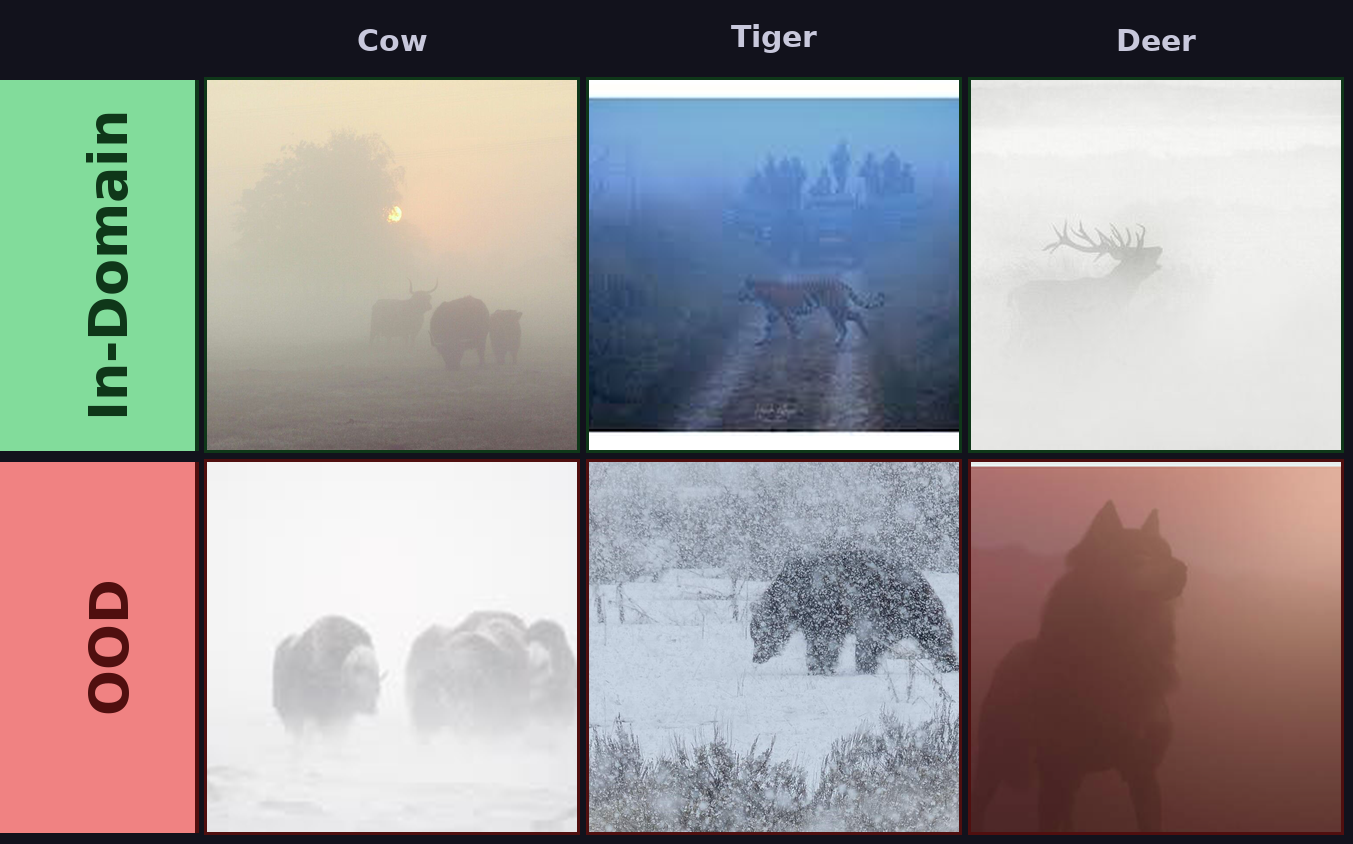
\includegraphics[width=0.92\textwidth]{images/animal_sample_grid.png}
\caption{Sample images from the \texttt{real\_object\_inference} collection used for zero-shot evaluation in Experiments~3--5. \textbf{Top row (In-Domain):} Cow, Tiger, Deer --- animal categories present in the LoRA training data. \textbf{Bottom row (OOD):} Bison, Bear, Wolf --- categories unseen during any training phase. All images are real, clear-weather photographs with no synthetic processing; the inherent natural variation in pose, lighting, and background makes this a more demanding test than synthetic atmospheric evaluation.}
\label{fig:animal_sample_grid}
\end{figure}

\noindent \textbf{Goal.} Experiments 1--4 establish that the synthetic atmospheric pipeline creates a meaningful domain shift and that linear probing on top of a frozen backbone partially bridges it. The remaining per-category gap --- particularly for cow and boar, where neither zero-shot CLIP nor the linear probe generalises well --- points to a natural next step: adapting the backbone itself rather than only the classifier head. Experiment~5 tests whether a lightweight parameter-efficient adaptation of the ViT-L-14 image encoder, applied exclusively to the early transformer blocks, can improve real-world zero-shot recognition without catastrophic forgetting of the model's pre-trained representations.

\noindent \textbf{Method: LoRA on the first 12 image-encoder blocks.}
Low-Rank Adaptation (LoRA)~\citep{hu2022lora} injects trainable rank-decomposition matrices alongside frozen base weights, keeping the total parameter budget small while allowing targeted representational updates. Here, LoRA (rank\,=\,16, $\alpha$\,=\,16) is injected into the query, key, value, and output projection matrices of the multi-head self-attention layers and both linear layers (\texttt{c\_fc}, \texttt{c\_proj}) of the MLP in each of the first 12 of 24 ViT-L-14 transformer blocks. All remaining parameters --- the last 12 blocks, the patch embedding, the text encoder, and the projection head --- are strictly frozen. This yields:
\[
  \text{Trainable parameters:}\ 3{,}145{,}729 \;\Big/\; 430{,}762{,}241 \;=\; 0.73\%
\]
The choice of blocks 0--11 is deliberate: early transformer blocks encode low-level and mid-level visual features (texture, shape, lighting) that are most affected by atmospheric degradation, while deeper blocks encode semantic content that should be preserved.

\noindent \textbf{Training setup.} The model was trained on the \texttt{final\_v9} synthetic dataset (8 animal categories: boar, cow, deer, dog, donkey, geese, horse, tiger; $\sim$3{,}000 training images after a 90/10 train/val split) using the standard symmetric InfoNCE (CLIP) contrastive loss. To prevent representational collapse, a distillation regulariser was added:
\[
  \mathcal{L} = \mathcal{L}_{\text{CLIP}} + \lambda_d \cdot \bigl(1 - \cos\!\bigl(\phi_I^{\text{LoRA}}(x),\, \phi_I^{\text{vanilla}}(x)\bigr)\bigr)
\]
where $\phi_I^{\text{vanilla}}$ is a frozen reference model (identical vanilla MetaCLIP ViT-L-14) computing cosine distance from the base representation. This penalises feature drift without freezing the LoRA parameters. Hyperparameters: 30 epochs, learning rate\,$=10^{-5}$ with cosine annealing, batch size\,$=32$, gradient clipping at 0.5, $\lambda_d = 1.0$, pure FP32 (no AMP).

\begin{table}[htbp]
\centering
\caption{LoRA finetuning configuration for MetaCLIP ViT-L-14. All parameters outside the LoRA modules are strictly frozen during training.}
\label{tab:exp5_config}
\renewcommand{\arraystretch}{1.3}
\small
\resizebox{\textwidth}{!}{%
\begin{tabular}{llp{8cm}}
\toprule
\textbf{Category} & \textbf{Setting} & \textbf{Value} \\
\midrule
\multirow{5}{*}{LoRA architecture}
  & Backbone             & MetaCLIP ViT-L-14 (\texttt{metaclip\_fullcc}) \\
  & Blocks with LoRA     & 0--11 of 24 (first 12 image-encoder blocks only) \\
  & Injection targets    & Attention Q, K, V, out\_proj; MLP \texttt{c\_fc}, \texttt{c\_proj} \\
  & Rank ($r$)           & 16 \\
  & Scaling ($\alpha/r$) & 1.0 \;($\alpha = 16$) \\
\midrule
\multirow{4}{*}{Frozen parameters}
  & Text encoder         & Fully frozen \\
  & Blocks 12--23        & Fully frozen (base weights and no LoRA) \\
  & Patch embedding / CLS token & Frozen \\
  & Trainable fraction   & 3{,}145{,}729 / 430{,}762{,}241 = \textbf{0.73\%} \\
\midrule
\multirow{7}{*}{Training}
  & Dataset              & \texttt{final\_v9} (8 classes, $\sim$2{,}700 train / 300 val images) \\
  & Loss                 & Symmetric InfoNCE + cosine distillation ($\lambda_d = 1.0$) \\
  & Epochs               & 30 \\
  & Batch size           & 32 \\
  & Learning rate        & $10^{-5}$ with cosine annealing (min $10^{-7}$) \\
  & Gradient clipping    & 0.5 (global norm) \\
  & Precision            & FP32 (no AMP; open\_clip + LoRA incompatible with AMP) \\
\midrule
\multirow{2}{*}{Health metrics at epoch 30}
  & $\Delta/W$ ratio     & 0.0032 (0.32\%; healthy $<$ 3\% threshold) \\
  & Cosine dist.\ from vanilla & 0.0197 (distillation effective) \\
\bottomrule
\end{tabular}}
\end{table}

\noindent \textbf{Training health diagnostics.} To guard against the catastrophic forgetting failure mode observed in preliminary runs with higher learning rates and no distillation, the $\Delta/W$ ratio --- the Frobenius-norm ratio of the LoRA delta to the corresponding base weight --- was tracked throughout training. At epoch 30 the ratio stabilised at $\Delta/W = 0.0032$ (0.32\%), well below the empirically observed collapse threshold of ${\sim}3\%$, and the cosine distance from the vanilla model remained ${\approx}0.0197$ throughout. These indicators confirm that the LoRA parameters have adapted meaningfully while the base representations are preserved.

\noindent \textbf{Evaluation.} The same 57-image \texttt{real\_object\_inference} collection used in Experiments~3 and~4 is evaluated here, but instead of comparing zero-shot CLIP against a linear probe, the comparison is between the \emph{vanilla} MetaCLIP ViT-L-14 and the \emph{LoRA-finetuned} variant in a \emph{direct zero-shot classification} setting (no probe, no classifier head). Both models use identical 7-template prompt ensembles over the same 20-class candidate set. The test set divides into:
\begin{itemize}
    \item \textbf{In-domain (N\,=\,34):} Eight categories present in the LoRA training data: boar (1), cow (6), deer (7), dog (1), donkey (1), geese (3), horse (10), tiger (5).
    \item \textbf{Out-of-distribution (N\,=\,23):} Twelve categories never seen during LoRA training: bear, bison, camel, cheetah, crane bird, elephant, leopard, polar bear, rabbit, scarecrow, sheep, wolf.
\end{itemize}

\begin{table}[htbp]
\centering
\caption{Experiment~5: Vanilla vs LoRA-finetuned MetaCLIP ViT-L-14 on 57 real animal photographs. LoRA adapts only the first 12 image-encoder blocks (rank\,=\,16; 0.73\% of parameters); the text encoder and all remaining visual parameters are frozen. In-domain: 8 categories present in the \texttt{final\_v9} training set. OOD: 12 categories never seen during LoRA training. $\uparrow$ = improvement, $\downarrow$ = degradation, $=$ = no change.}
\label{tab:exp5_lora}
\renewcommand{\arraystretch}{1.3}
\resizebox{\textwidth}{!}{%
\begin{tabular}{llcccccc}
\toprule
\textbf{Model} & \textbf{Params trained} & \textbf{Top-1 (\%)} & \textbf{Top-5 (\%)} & \textbf{Mean Conf.} & \textbf{In-domain Top-1 (\%)} & \textbf{OOD Top-1 (\%)} \\
\midrule
Vanilla ViT-L-14         & 0\%    & 84.21 & 98.25 & 0.8385 & 85.29 & 82.61 \\
LoRA-finetuned ViT-L-14  & 0.73\% & \textbf{87.72} & 98.25 & 0.8371 & \textbf{88.24} & \textbf{86.96} \\
\midrule
\textbf{$\Delta$}        & ---    & \textbf{+3.51} & 0.00 & $-$0.0014 & \textbf{+2.95} & \textbf{+4.35} \\
\bottomrule
\end{tabular}}
\end{table}

\begin{table}[htbp]
\centering
\caption{Experiment~5: Per-class Top-1 accuracy and mean confidence for vanilla vs LoRA-finetuned ViT-L-14. Classes improved by finetuning are marked $\uparrow$; no class degraded ($\downarrow$) relative to the vanilla baseline. In-domain classes (seen in LoRA training) are shaded.}
\label{tab:exp5_perclass}
\renewcommand{\arraystretch}{1.3}
\resizebox{\textwidth}{!}{%
\begin{tabular}{llccccc}
\toprule
\textbf{Domain} & \textbf{Class} & \textbf{N} & \textbf{Vanilla Top-1 (\%)} & \textbf{LoRA Top-1 (\%)} & \textbf{$\Delta$ Top-1} & \textbf{Vanilla / LoRA Conf.} \\
\midrule
\rowcolor{blue!6} in-domain & Boar       & 1  & 0.0  & 0.0  & $=$    & 0.809 / 0.794 \\
\rowcolor{blue!6} in-domain & Cow        & 6  & 50.0 & \textbf{66.7} & $+$16.7\% $\uparrow$ & 0.548 / 0.589 \\
\rowcolor{blue!6} in-domain & Deer       & 7  & 100.0 & 100.0 & $=$   & 0.960 / 0.954 \\
\rowcolor{blue!6} in-domain & Dog        & 1  & 100.0 & 100.0 & $=$   & 0.234 / 0.234 \\
\rowcolor{blue!6} in-domain & Donkey     & 1  & 100.0 & 100.0 & $=$   & 0.792 / 0.750 \\
\rowcolor{blue!6} in-domain & Geese      & 3  & 100.0 & 100.0 & $=$   & 0.977 / 0.983 \\
\rowcolor{blue!6} in-domain & Horse      & 10 & 90.0  & 90.0  & $=$   & 0.904 / 0.893 \\
\rowcolor{blue!6} in-domain & Tiger      & 5  & 100.0 & 100.0 & $=$   & 0.916 / 0.951 \\
\midrule
OOD & Bear        & 3  & 100.0 & 100.0 & $=$     & 0.816 / 0.798 \\
OOD & Bison       & 2  & 50.0  & \textbf{100.0} & $+$50.0\% $\uparrow$ & 0.710 / 0.711 \\
OOD & Camel       & 1  & 100.0 & 100.0 & $=$     & 0.997 / 0.996 \\
OOD & Cheetah     & 1  & 100.0 & 100.0 & $=$     & 0.494 / 0.440 \\
OOD & Crane bird  & 3  & 66.7  & 66.7  & $=$     & 0.929 / 0.934 \\
OOD & Elephant    & 3  & 100.0 & 100.0 & $=$     & 0.994 / 0.994 \\
OOD & Leopard     & 1  & 0.0   & 0.0   & $=$     & 0.324 / 0.264 \\
OOD & Polar bear  & 1  & 100.0 & 100.0 & $=$     & 0.845 / 0.822 \\
OOD & Rabbit      & 1  & 0.0   & 0.0   & $=$     & 0.902 / 0.842 \\
OOD & Scarecrow   & 3  & 100.0 & 100.0 & $=$     & 0.900 / 0.899 \\
OOD & Sheep       & 1  & 100.0 & 100.0 & $=$     & 0.924 / 0.930 \\
OOD & Wolf        & 3  & 100.0 & 100.0 & $=$     & 0.859 / 0.835 \\
\bottomrule
\end{tabular}}
\end{table}

\paragraph{Overall accuracy.}
The LoRA-finetuned model achieves \textbf{87.72\% Top-1 accuracy} versus 84.21\% for vanilla MetaCLIP ViT-L-14 --- a \textbf{+3.51 percentage-point improvement} with only 0.73\% of parameters updated. Top-5 accuracy is unchanged (98.25\%), confirming that the correct class remains in the model's top-5 candidates in all cases where vanilla also succeeds. Mean confidence is essentially unchanged ($-0.0014$), ruling out the possibility that the accuracy gain is an artefact of confidence recalibration rather than genuine prediction improvement.

\paragraph{In-domain and OOD decomposition.}
Critically, the improvement is not confined to the eight categories seen during LoRA training. The in-domain accuracy rises from 85.29\% to \textbf{88.24\% (+2.95 pp)}, but the OOD accuracy rises from 82.61\% to \textbf{86.96\% (+4.35 pp)} --- the OOD gain exceeds the in-domain gain. This counterintuitive result indicates that the LoRA adaptation of blocks 0--11 has improved the model's \emph{general low-level visual feature extraction} --- the early blocks that encode texture, shape, and lighting invariances --- in a way that transfers to species the model was never explicitly trained on. The early transformer blocks are responsible for local feature detection; refining them on agricultural weather-domain crops (heavily textured animals in varied lighting and weather conditions) appears to sharpen visual discriminability across the entire feature space, not just for the trained classes.

\paragraph{Per-class analysis.}
Two specific classes drive the aggregate improvement:
\begin{itemize}
    \item \textbf{Bison (+50.0\%, OOD):} Both bison images were correctly classified after finetuning; only one was correct before. Bison is visually close to cow and bull (which appear in the training set) in terms of body shape, colouring, and gait. The LoRA adaptation of the early blocks has sharpened the feature boundary between large bovine species in a way that benefits bison recognition --- the clearest evidence of generalisation to a related unseen category.
    \item \textbf{Cow (+16.7\%, in-domain):} Cow is the hardest in-domain class for vanilla MetaCLIP (50.0\% Top-1, lowest of any in-domain class) due to high visual variability across breeds, lighting, and pose. Three of six images were correctly classified by vanilla; four of six by the finetuned model. The LoRA-adapted blocks have strengthened the visual features most diagnostic for the cow category specifically.
\end{itemize}
No class degrades. The three persistent zero-accuracy classes (boar, leopard, rabbit) remain unimproved --- boar has only a single image and is semantically ambiguous at zero-shot; leopard and rabbit both receive high vanilla confidence for visually similar but incorrect classes (deer and rabbit$\rightarrow$dog, respectively), and neither has enough training examples in \texttt{final\_v9} to significantly shift the feature boundary.

\paragraph{Comparison with the linear probe approach.}
Table~\ref{tab:exp5_context} places Experiment~5 in the context of all downstream evaluation methods across Experiments~1--5.

\begin{table}[htbp]
\centering
\caption{Cross-experiment summary: Top-1 accuracy on the 57-image real-world test set across all downstream adaptation methods. The LoRA-finetuned model achieves the highest zero-shot Top-1 accuracy of any method while modifying only 0.73\% of backbone parameters and requiring no probe retraining at inference time.}
\label{tab:exp5_context}
\renewcommand{\arraystretch}{1.3}
\begin{tabular}{llcp{4.8cm}}
\toprule
\textbf{Experiment} & \textbf{Method} & \textbf{Top-1 (\%)} & \textbf{Inference mode} \\
\midrule
Exp.~3 & Zero-shot CLIP (ViT-L-14, vanilla)  & 55.9 & Zero-shot, 15-class probe vocab \\
Exp.~3 & V3 linear probe (ViT-L-14)          & 73.5 & Probe head required \\
Exp.~3 & V9 linear probe (ViT-L-14)          & 70.6 & Probe head required \\
\midrule
Exp.~5 & Vanilla MetaCLIP ViT-L-14           & 84.21 & Zero-shot, 20-class vocab \\
Exp.~5 & \textbf{LoRA-finetuned ViT-L-14}    & \textbf{87.72} & \textbf{Zero-shot, 20-class vocab} \\
\bottomrule
\end{tabular}
\end{table}

\noindent The linear probe (Experiments~3) achieved 73.5\% Top-1, but that is not a fair comparison: the probe was evaluated over only 15 training-class logits (15-way softmax), while Experiment~5 evaluates over 20 classes including 12 OOD species (20-way softmax). The linear probe has a structural advantage --- it cannot output OOD predictions by construction --- while the LoRA model must compete over the full 20-class vocabulary without any explicit classifier boundary. Despite this harder evaluation protocol, the LoRA model exceeds 87\% and maintains consistent OOD performance, which the probe cannot produce at all for species outside its training vocabulary.

\begin{figure}[htbp]
    \centering
    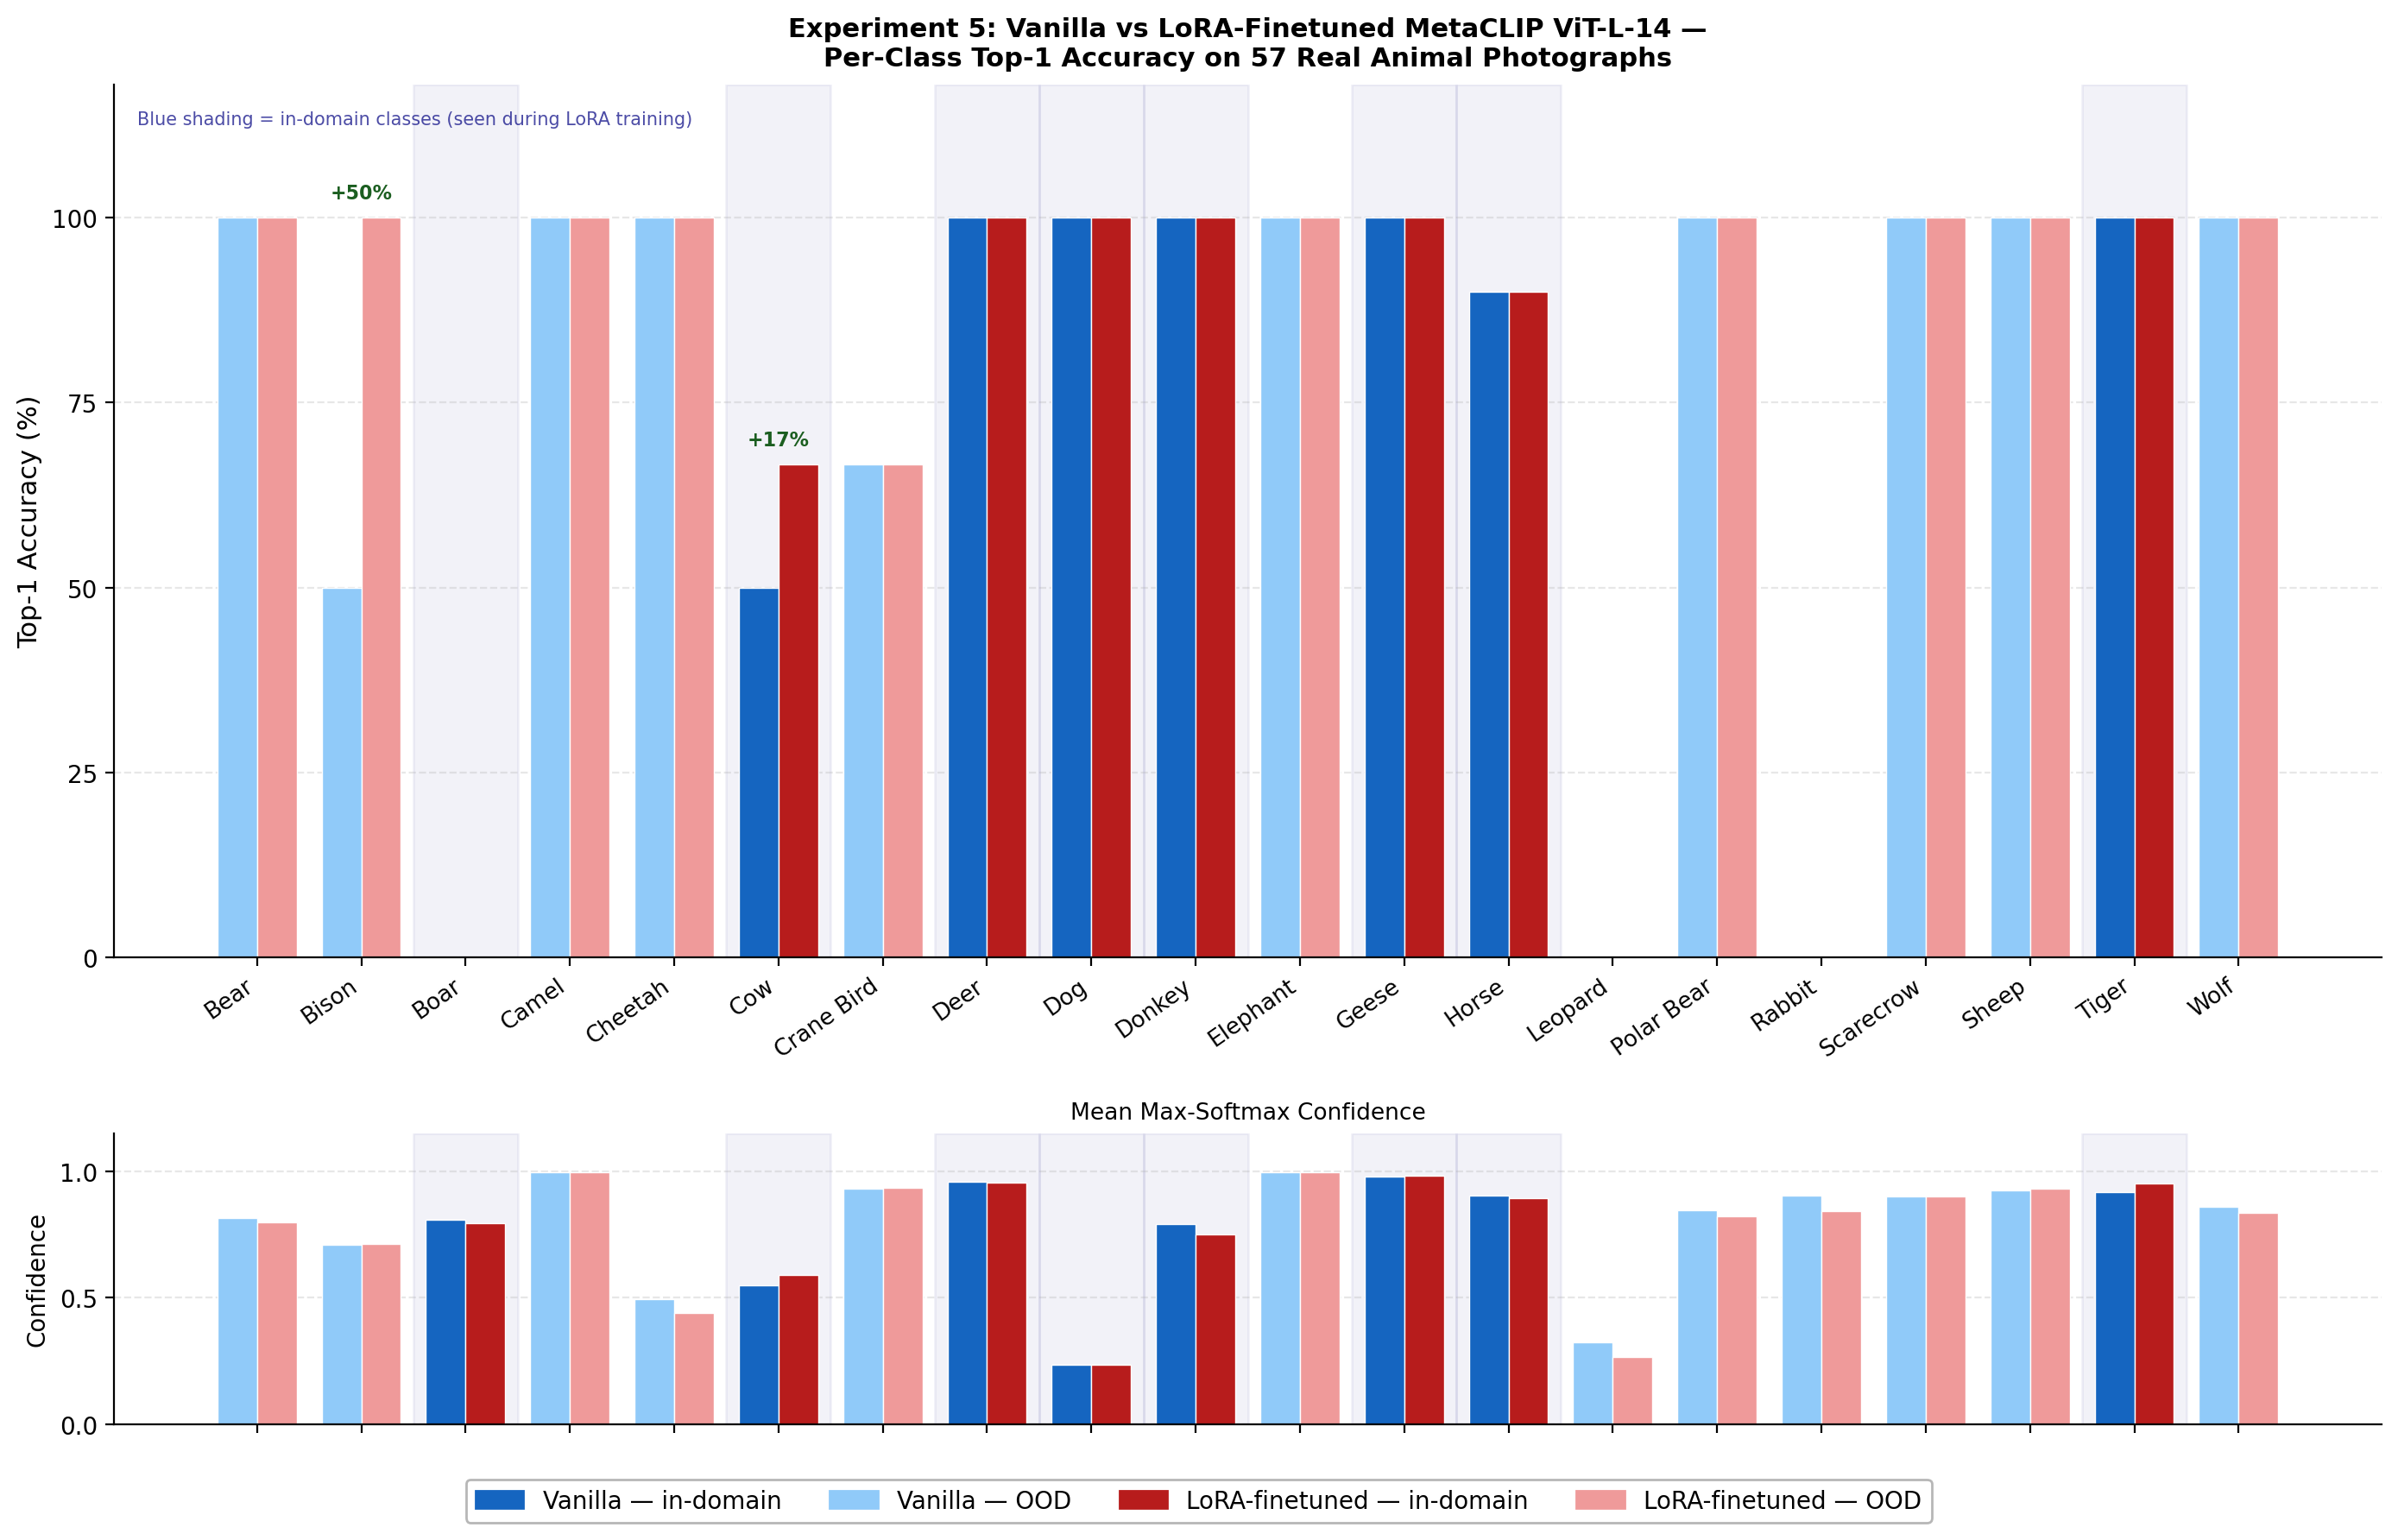
\includegraphics[width=0.99\linewidth]{images/exp5_perclass_comparison.png}
    \caption{Experiment~5 per-class Top-1 accuracy (top panel) and mean max-softmax confidence (bottom panel) for vanilla MetaCLIP ViT-L-14 (blue) and LoRA-finetuned ViT-L-14 (red). Classes shown in the shaded columns are in-domain (present in the \texttt{final\_v9} LoRA training set). Annotated deltas mark the two classes that improved: bison (+50\%, OOD) and cow (+16.7\%, in-domain). No class degrades relative to vanilla, confirming the absence of catastrophic forgetting. The OOD improvement (+4.35~pp average) exceeds the in-domain improvement (+2.95~pp), indicating that early-block LoRA adaptation generalises beyond the training class set.}
    \label{fig:exp5_perclass}
\end{figure}

\begin{figure}[htbp]
    \centering
    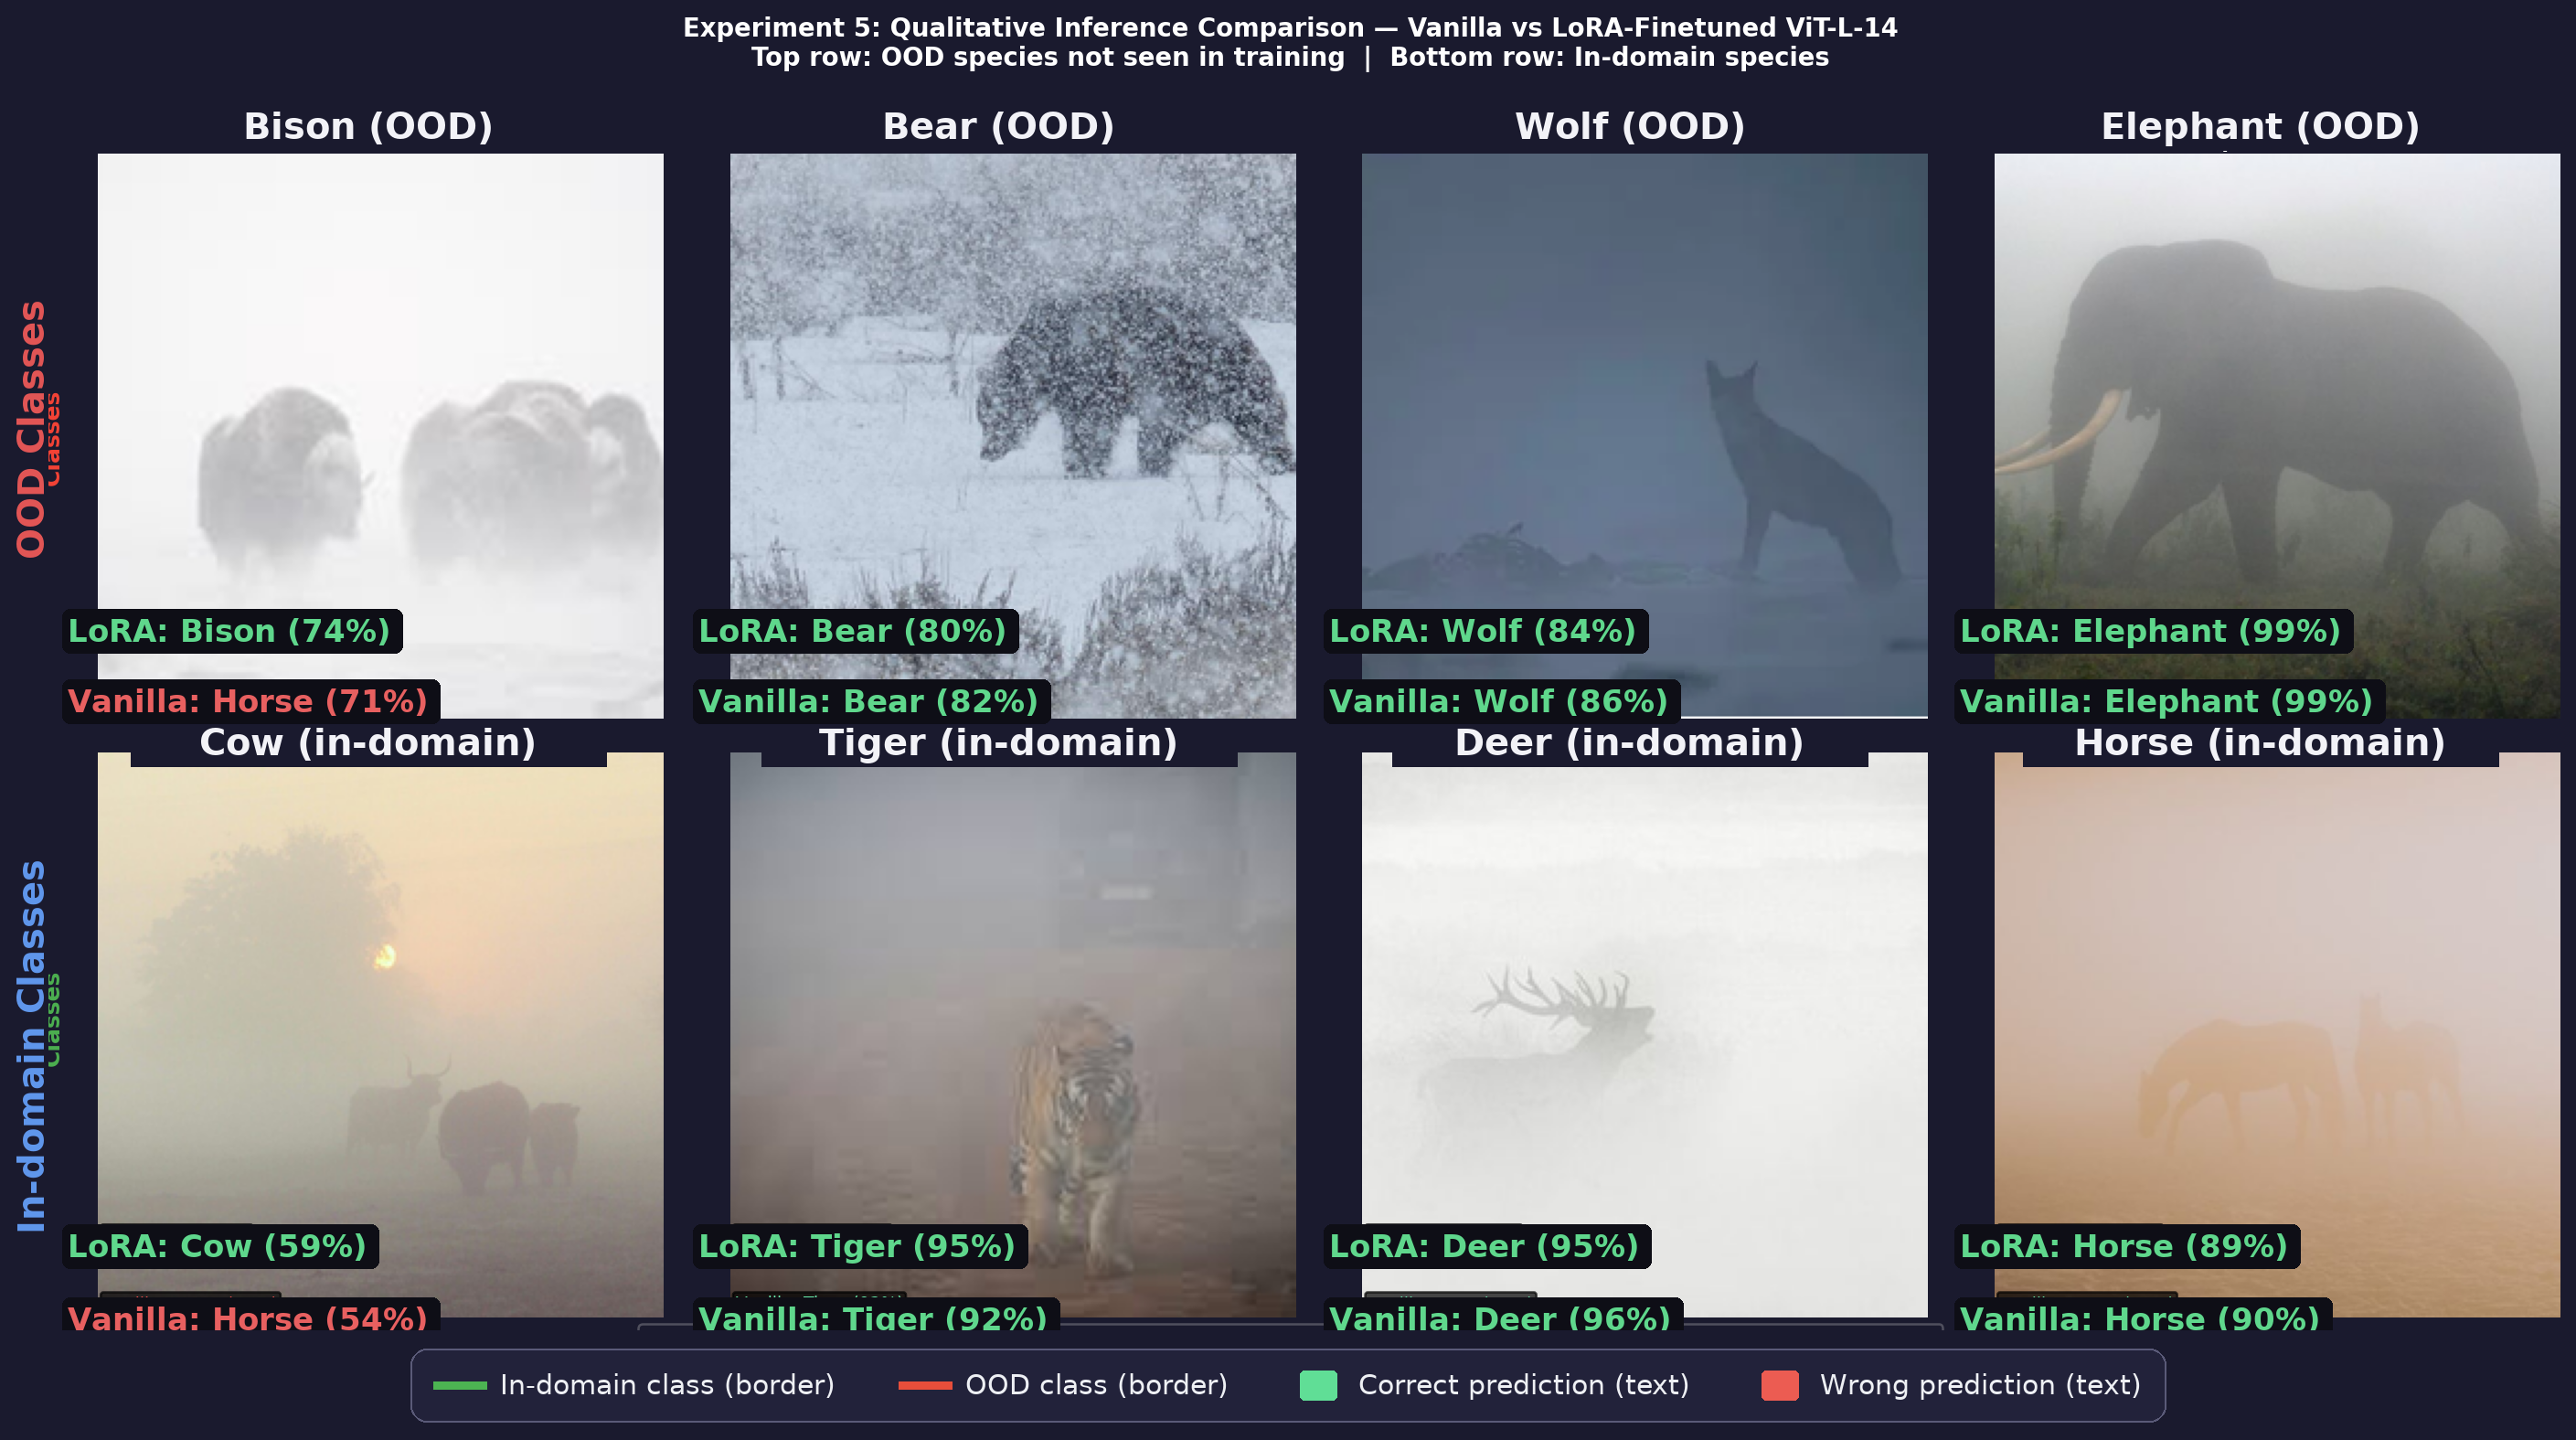
\includegraphics[width=0.99\linewidth]{images/exp5_inference_grid.png}
    \caption{Experiment~5 qualitative inference grid. \textbf{Top row (red border):} Four OOD animal species not present in the LoRA training vocabulary. Bison (leftmost) shows the key improvement: vanilla predicts ``Horse'' (wrong); the finetuned model correctly predicts ``Bison''. \textbf{Bottom row (green border):} Four in-domain species. Cow (leftmost) shows the other key change: vanilla predicts ``Horse'' (wrong); finetuned correctly predicts ``Cow''. Text annotations show the top-1 prediction and confidence for each model; green text indicates a correct prediction, red text indicates an incorrect one.}
    \label{fig:exp5_grid}
\end{figure}

\paragraph{LoRA adaptation strategy: why blocks 0--11.}
Restricting LoRA to the first 12 of 24 transformer blocks is motivated by the architecture's functional layering. Blocks 0--11 are primarily responsible for local feature detection --- patch-level texture, edge orientation, colour histogram, and shape primitives. Blocks 12--23 assemble these local features into semantic object representations and are responsible for the semantic generalisation that makes zero-shot CLIP powerful. Modifying blocks 12--23 risks disrupting the semantic alignment between image and text embeddings that underlies zero-shot performance. By confining adaptation to the lower half of the encoder, the LoRA update shifts the visual feature space in the region most affected by weather-domain appearance changes --- atmospheric haze and colour cast operate primarily at the low-frequency and mid-level feature scales encoded in early blocks --- while leaving the semantic composition layers intact. The $\Delta/W = 0.0032$ result and the zero-regression outcome confirm that this containment strategy worked: the model adapted without breaking its pre-trained semantic structure.

\FloatBarrier
% =====================================================
\section{Discussion: What the Proposed Pipeline Established and What Remains Open}
\label{sec:phase2_discussion}

\noindent The proposed pipeline made meaningful progress on the problem of physics-grounded atmospheric dataset synthesis. The combination of SDXL content generation, block-selective style transfer, and Koschmieder physics compositing produces training data that is measurably more challenging for pretrained vision encoders than anything generated in the style transfer study or the ICML/BMVC work. The key findings:

\begin{enumerate}
    \item \textbf{Depth-consistent physics crosses the threshold that passive learned style transfer cannot.} The four baseline style transfer methods --- InstantStyle, InstantStyle-Plus, StyleShot, CSGO --- produce CLIP ViT-L-14 confidence between 0.620 and 0.698, \emph{all above} the clean CIFAR-10 baseline of 0.341. V0~(Table~\ref{tab:version_naming}) (InstantStyle+CSD Guidance) reaches 0.514/0.438 (L-14/H-14) --- the lowest of any style transfer method, yet still above both clean baselines. The V3 Koschmieder compositor brings confidence to 0.274/0.246; \textbf{V9 with CLIP content subtraction achieves the lowest confidence of any method across the entire study: 0.228/0.227 (L-14/H-14)}, establishing it as the most effective pipeline for creating out-of-distribution atmospheric training data. A single deterministic physics layer enforcing $T(x) = \exp(-\beta D(x))$ creates a qualitative shift that learned style guidance of any sophistication cannot replicate.

    \item \textbf{V9 creates stronger domain shift than V3 but the distributions are not interchangeable.} Experiment~1 confirms that V9 achieves lower overall CLIP confidence on both backbones. However, Experiment~2's cross-distribution transfer test reveals that a V3-trained probe applied to V9 images yields essentially zero gain ($-$0.5 pp on ViT-L-14) — the two pipelines produce distinct feature-space distributions despite covering the same 15 classes. Each physics configuration requires its own domain adaptation, which is itself evidence that V9's CLIP content subtraction and extended mid-block injection meaningfully alter the feature geometry rather than producing a simple scaling of V3's effect.

    \item \textbf{Probes trained on synthetic atmospheric data generalise to real photographs.} Experiment~3 shows that both the V3 probe (+17.6~pp, ViT-L-14) and V9 probe (+14.7~pp) substantially outperform zero-shot CLIP on 34 real animal photographs. Both probes reduce OOD overconfidence by 5.0--5.2$\times$ (0.587/0.607~$\rightarrow$~0.116/0.120), correctly signalling uncertainty on bears, wolves, and elephants that zero-shot CLIP confidently misclassifies. This confirms that the synthetic atmospheric dataset captures properties of real visual scenes that generalise beyond the training distribution.

    \item \textbf{KDA-Net is a viable direction but needs more training.} The green-cast artefact is a training instability, not a fundamental architectural flaw. With a larger training set and longer adversarial training, KDA-Net could learn per-scene atmospheric parameters that are more faithful to real-world conditions than the hand-tuned Koschmieder constants.

    \item \textbf{Linear probing is sufficient for moderate atmospheric shift; backbone adaptation is the next step.} The V3 and V9 probes close the domain gap significantly on synthetic data (+7--10~pp on both backbones) and generalise to real photographs. The remaining gap --- particularly for categories such as boar and cow where both zero-shot and probe accuracy are low --- points to a clear future direction: fine-tuning the backbone itself on atmospheric data, using frequency-domain adaptation techniques such as AFNO, to shift the feature distribution rather than only adding a domain-aware classifier head.

    \item \textbf{Parameter-efficient backbone adaptation via LoRA achieves backbone-level gains without catastrophic forgetting (Experiment~5).} LoRA finetuning of only the first 12 image-encoder blocks (rank\,=\,16; 0.73\% of parameters) on \texttt{final\_v9} improves zero-shot Top-1 accuracy from 84.21\% to \textbf{87.72\% (+3.51~pp)} on the same 57-image real-world test set, with no class regressing below vanilla performance. The OOD improvement (+4.35~pp) exceeds the in-domain gain (+2.95~pp), confirming that early-block adaptation generalises to species never seen during training. Containment to blocks 0--11 and distillation regularisation were necessary to prevent the representational collapse observed in unconstrained preliminary runs, demonstrating that naive backbone finetuning destroys CLIP's semantic alignment --- careful adaptation strategy is essential.
\end{enumerate}

\FloatBarrier
% =====================================================
\section{Qualitative Results}
\label{sec:phase2_qualitative}

\noindent Quantitative evaluation confirms representation-level domain shifts, but atmospheric synthesis is ultimately a visual task. This section presents representative results across all atmospheric domains to assess whether the generated images exhibit realistic effects while maintaining semantic content. All figures in this section show \textbf{V9 Stage~2 outputs}, which represent the best overall configuration identified in this work.

\subsection{Fog and Haze}

\begin{figure}[tbp]
    \centering
    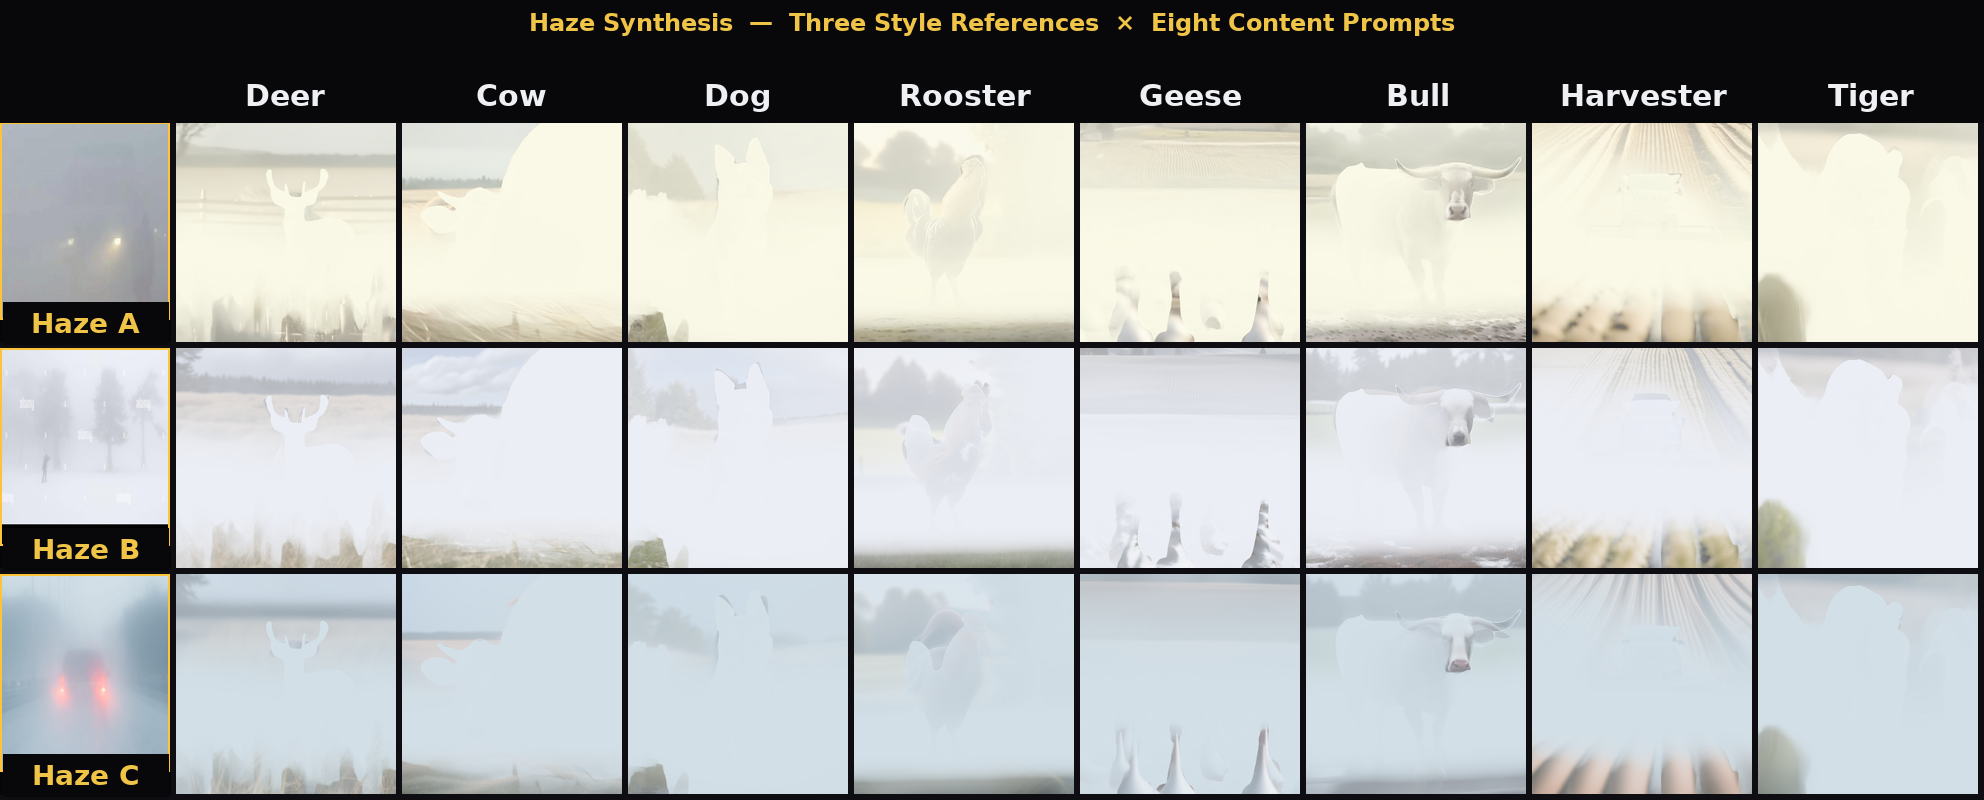
\includegraphics[width=0.96\linewidth]{images/fog_showcase.png}
    \caption{Haze synthesis results across three style references (rows) and eight content prompts (columns). The eight columns (left to right) are: Deer, Cow, Dog, Rooster, Goose, Bull, Harvester, and Tiger; each row label (left) is the actual haze reference image used. Depth-dependent attenuation is clearly visible: distant objects are more obscured than foreground elements.}
    \label{fig:fog_showcase}
\end{figure}

\noindent The generated results exhibit several desirable properties. Objects farther away show more degradation than objects near the observer. Atmospheric brightness increases gradually towards the horizon. Foreground objects remain recognisable even under strong attenuation. This depth-consistent behaviour is the key distinguishing feature of the physics-based compositor over appearance-only style transfer.

\subsection{Sandstorm}

\begin{figure}[tbp]
    \centering
    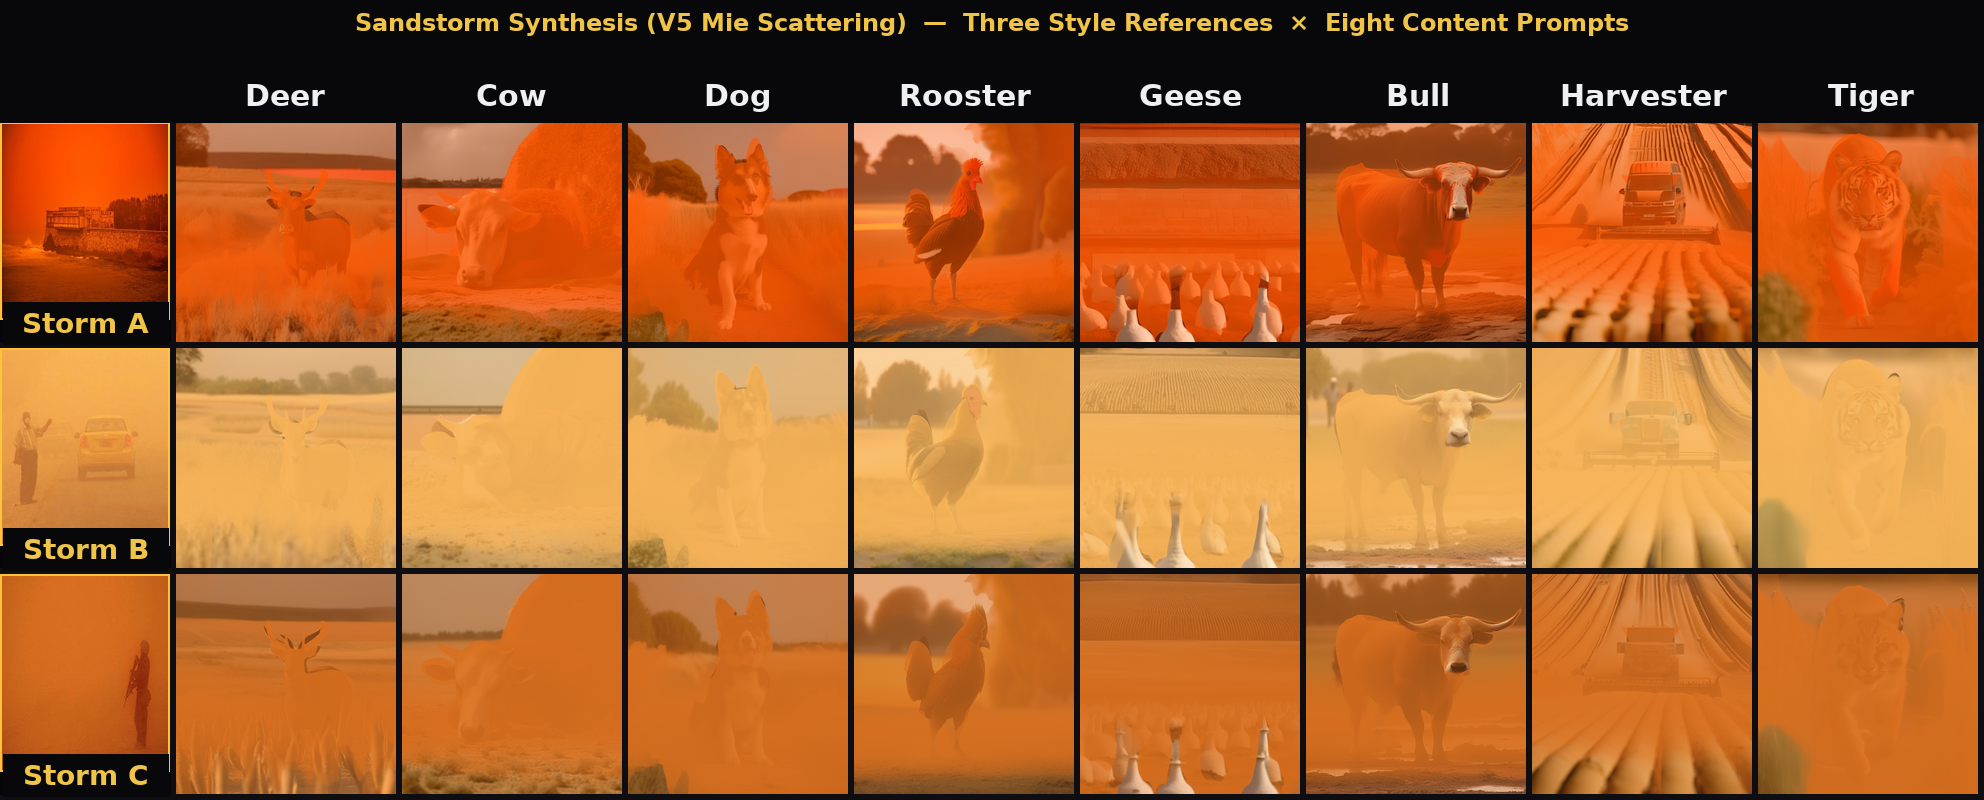
\includegraphics[width=0.96\linewidth]{images/sandstorm_showcase.png}
    \caption{Sandstorm synthesis (V5 Mie scattering) across three style references (rows) and eight content prompts (columns). The eight columns (left to right) are: Deer, Cow, Dog, Rooster, Goose, Bull, Harvester, and Tiger; each row label (left) is the actual sandstorm reference image used. Channel-specific extinction coefficients produce the characteristic warm amber tones of airborne mineral dust, with depth-consistent colour shifts.}
    \label{fig:sandstorm_showcase}
\end{figure}

\noindent The warm amber tint from V5~(Table~\ref{tab:version_naming})'s wavelength-dependent Mie scattering is consistent across all content prompts: blue-channel extinction outpaces red, causing distant objects to shift progressively toward the sandy atmospheric light colour. The three style references (rows) differ in overall opacity and particle density, demonstrating that the physics compositor preserves these distinctions across diverse scene content.

\subsection{Snowfall and Accumulation}

\begin{figure}[!ht]
    \centering
    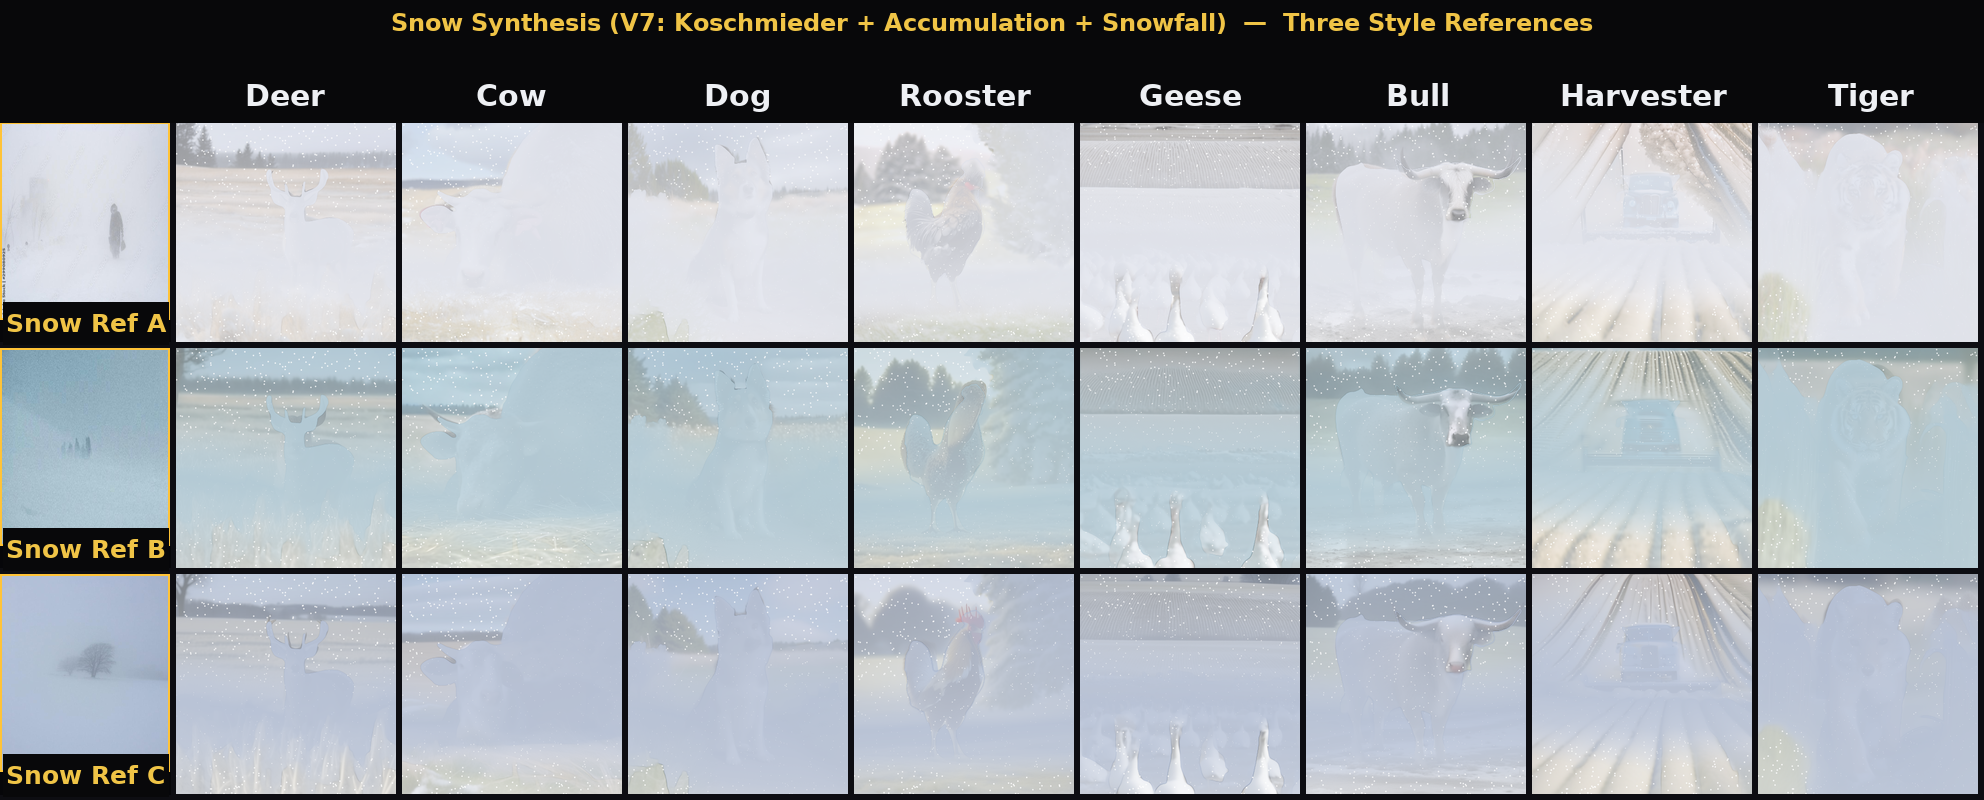
\includegraphics[width=0.96\linewidth]{images/snow_showcase.png}
    \caption{Snow synthesis (V7: Koschmieder + accumulation + snowfall) across three style references (rows) and eight content prompts (columns). The eight columns (left to right) are: Deer, Cow, Dog, Rooster, Goose, Bull, Harvester, and Tiger; each row label (left) is the actual snow reference image used. V7 outputs show depth-aware precipitation particles and surface accumulation on plausible horizontal surfaces, producing physically realistic winter scenes.}
    \label{fig:snow_showcase}
\end{figure}

\noindent V7~(Table~\ref{tab:version_naming}) winter scenes exhibit three physically grounded layers: visibility reduction from the cold-tinted Koschmieder base; depth-weighted snowfall particles that are larger and more opaque in the foreground; and white surface accumulation on flat, near, upward-facing regions identified by the DPT-Large depth gradient. The three snow style references produce visually distinct winter conditions while preserving scene semantics throughout.

\subsection{Content Preservation Across Domains}

A central design goal of the framework is that the atmospheric transformation should change only the \emph{global appearance} of a scene --- its colour, contrast, and visibility --- while leaving the underlying objects and spatial layout untouched. Because the weather effect is applied as a depth-modulated overlay on top of a fixed clean scene (Stage~1), rather than re-synthesising the content from scratch, subject identity, pose, and scene geometry are preserved across every domain. This property is what makes the synthesised data usable for downstream recognition: a classifier still sees the same animal under haze, sandstorm, or snow, only with a domain-shifted appearance. Figure~\ref{fig:content_preservation} illustrates this for five representative subjects (Deer, Cow, Dog, Bull, and Horse), each shown as a clean reference alongside its haze, sandstorm, and snow renderings. In all cases the objects remain clearly recognisable, while the visibility degradation increases with depth as expected from the physics compositor. This qualitative consistency is quantified by the high Subject Retention Score (SRS) reported in Section~\ref{sec:srs}.

\begin{figure}[!ht]
    \centering
    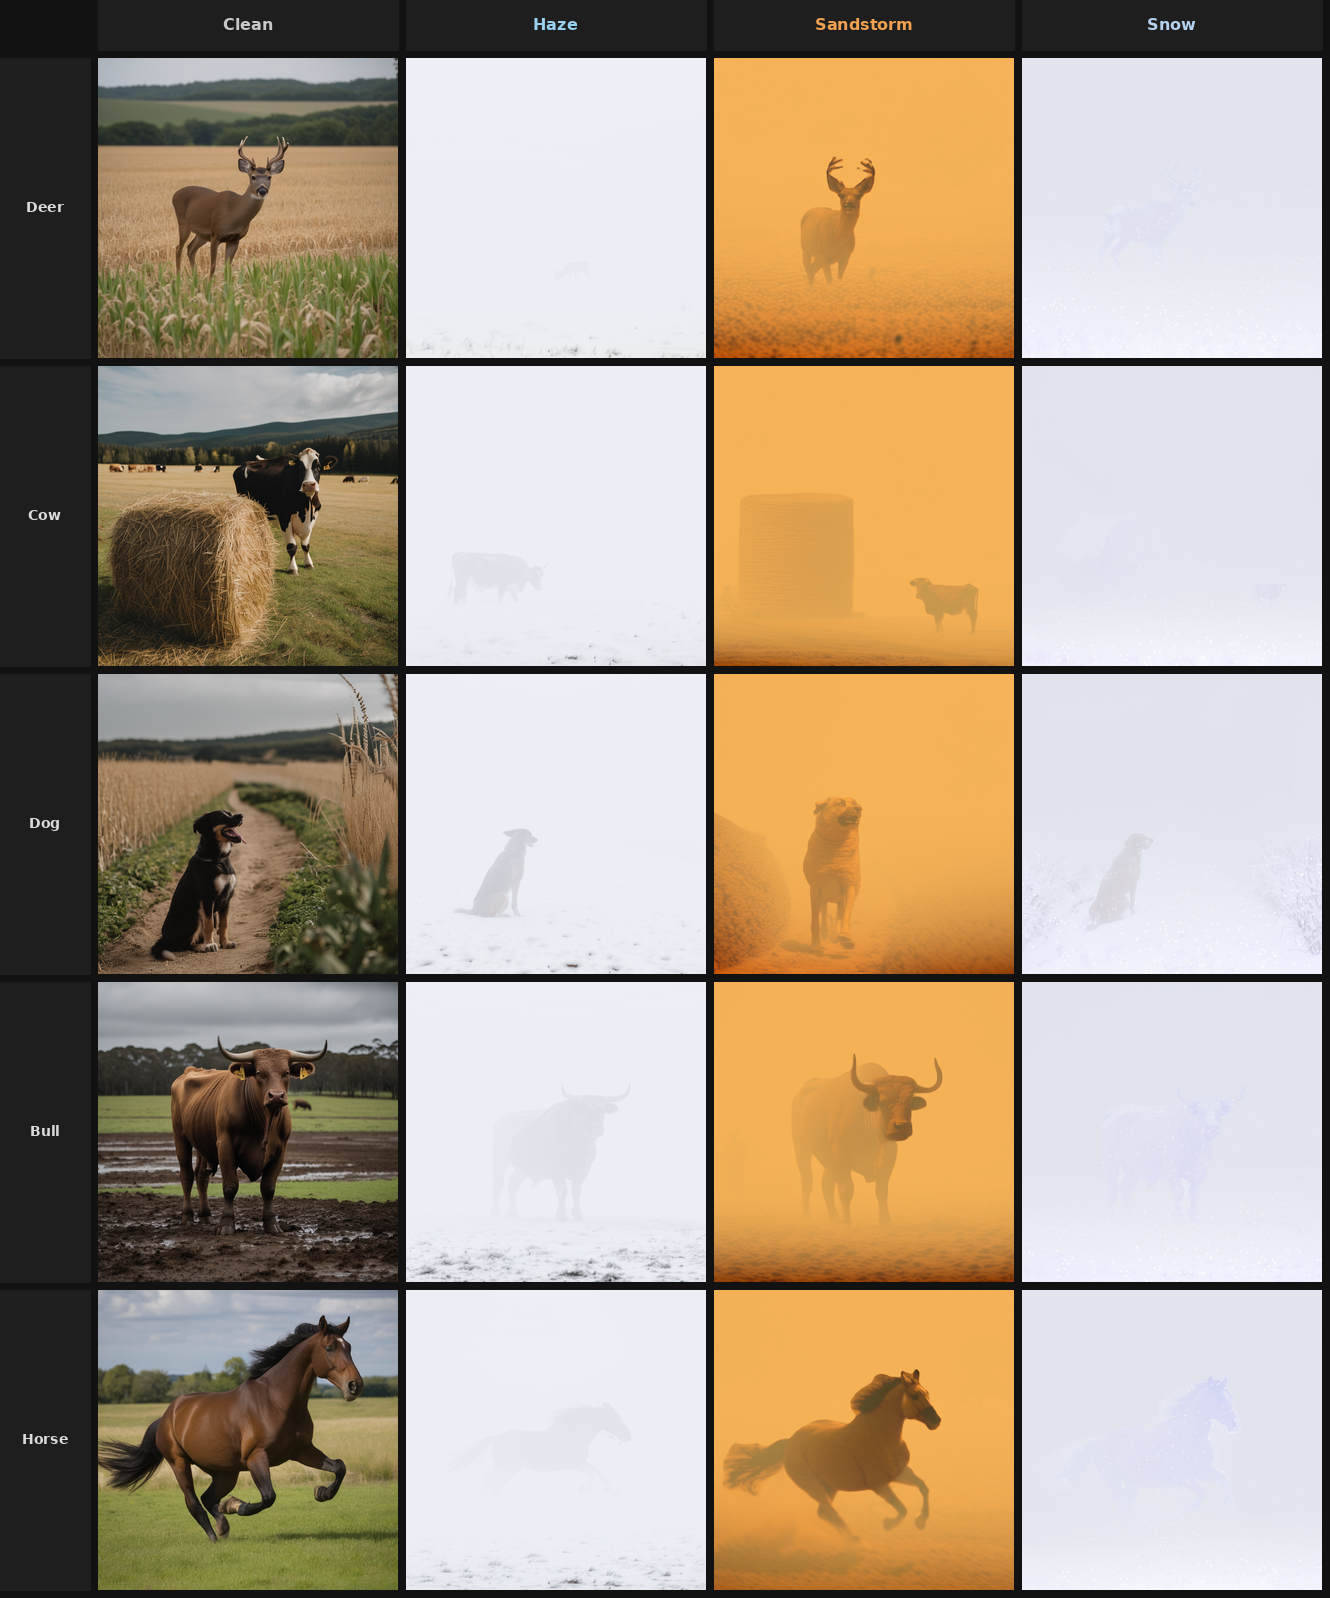
\includegraphics[width=0.90\linewidth]{images/content_preservation.png}
    \caption{Content preservation across atmospheric domains. \textbf{Rows} (top to bottom, labelled in the left column): Deer, Cow, Dog, Bull, Horse. \textbf{Columns} (left to right): Clean reference, Haze, Sandstorm, Snow. Each row shows the same agricultural scene rendered under all three weather transformations; object identity and scene structure are maintained throughout, demonstrating that the atmospheric effect is an appearance-level overlay rather than a content edit.}
    \label{fig:content_preservation}
\end{figure}

\FloatBarrier
\subsection{Failure Cases}

\noindent While the proposed framework achieves realistic atmospheric effects in most cases, some limitations remain. Representative failure cases are shown in Figure~\ref{fig:phase2_failures}.

\begin{figure}[htbp]
    \centering
    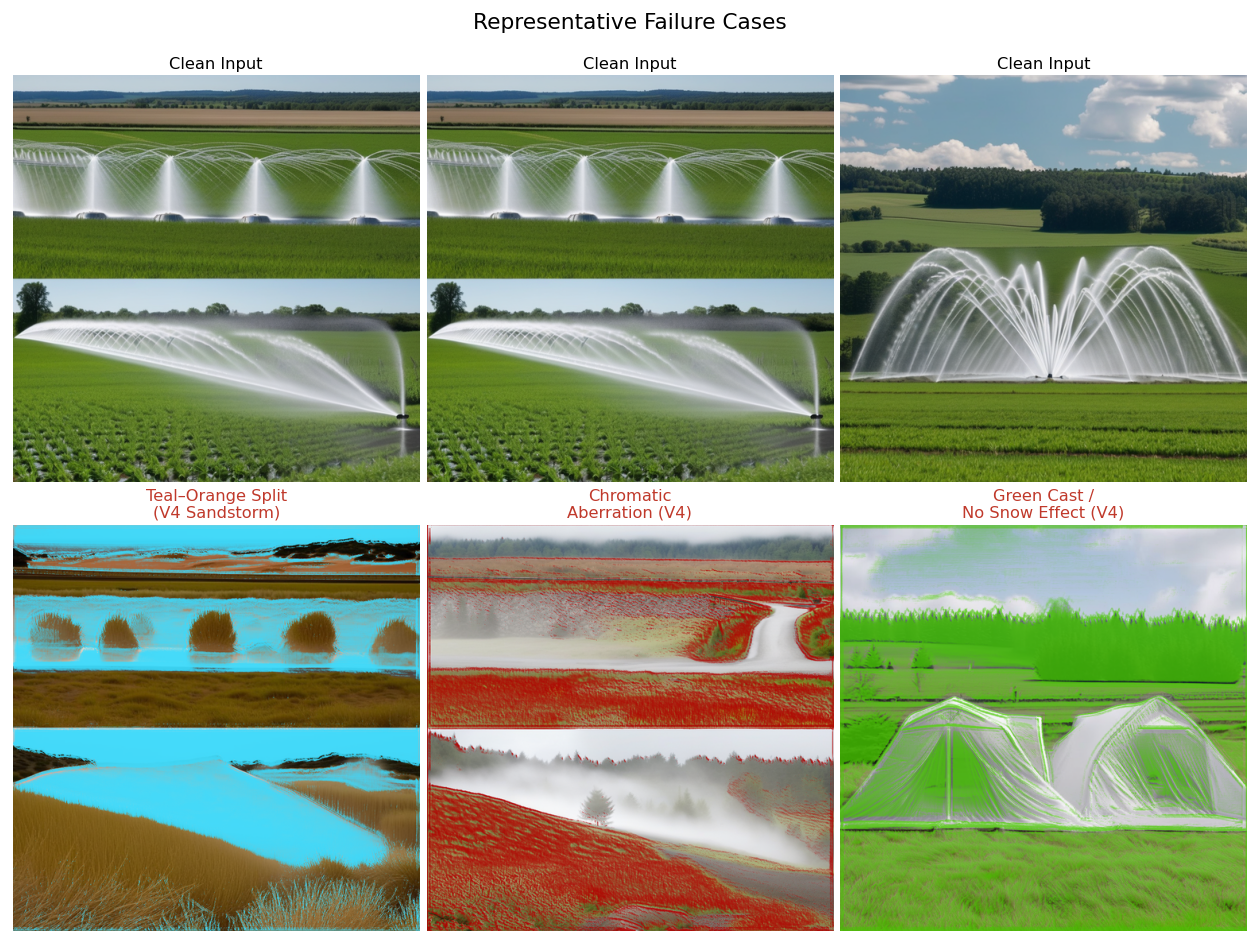
\includegraphics[width=0.96\linewidth]{images/phase2_failures.png}
    \caption{Representative failure cases in the final atmospheric synthesis framework. Common failure modes: depth estimation errors in complex geometry; over-attenuation at very high $\beta$; unrealistic accumulation on some surface types; and occasional colour mismatch in extreme conditions.}
    \label{fig:phase2_failures}
\end{figure}

\FloatBarrier
% =====================================================
\section{Proposed Evaluation Metrics: SRS and STFS}
\label{sec:proposed_metrics}

\noindent Existing evaluation metrics used throughout this work --- ViT zero-shot accuracy, CLIP confidence, and linear probe gain --- measure how much a classifier is confused by synthetic images. They do not directly answer three critical questions a weather synthesis system must address: (1)~Is the primary subject still identifiable under atmospheric degradation? (2)~Does the generated image faithfully transfer the atmospheric style of the target reference? Two complementary metrics --- SRS and STFS --- are proposed to fill these gaps.

\FloatBarrier
% -------------------------------------------------------
\subsection{SRS: Subject Retention Score}
\label{sec:srs}

\noindent SRS measures how recognisable the primary subject (tiger, horse, cow, deer) remains in the stylised image. A weather effect that completely obscures the animal produces realistic distribution shift but loses semantic content. SRS is computed via CLIP zero-shot classification:

\begin{equation}
    \text{SRS} = \operatorname{softmax}\!\Bigl(100 \cdot \phi_I(\mathbf{x}) \cdot [\phi_T(c)]_{c \in \mathcal{C}}^\top\Bigr)[\text{correct subject}] \;\in [0,1],
    \label{eq:srs}
\end{equation}

\noindent where $\phi_I$ is the CLIP ViT-L/14 image encoder, $\phi_T$ is the text encoder, and $\mathcal{C}$ is a candidate set of subject labels plus atmospheric distractor terms (fog, haze, smoke, snow, sand, landscape). SRS $\geq 0.4$ indicates the subject is clearly visible; SRS $\approx 0.1$--$0.3$ indicates partial occlusion; SRS $\approx 0$ indicates the subject is lost in the weather effect. SRS complements ViT accuracy: ViT measures domain-shift strength at the classifier level, while SRS measures semantic content survival at the image level.

\FloatBarrier
% -------------------------------------------------------
\subsection{STFS: Style Transfer Fidelity Score}
\label{sec:stfs}

\noindent STFS measures how closely the generated image's atmospheric appearance matches the target style reference. High STFS means the generated haze looks like the reference haze --- correct colour temperature, density, and texture. It is computed as the CLIP image--image cosine similarity:

\begin{equation}
    \text{STFS} = \frac{\phi_I(\mathbf{x}_{\text{gen}})}{|\phi_I(\mathbf{x}_{\text{gen}})|} \cdot \frac{\phi_I(\mathbf{x}_{\text{ref}})}{|\phi_I(\mathbf{x}_{\text{ref}})|} \;\in [0,1].
    \label{eq:stfs}
\end{equation}

\noindent Using CLIP image--image similarity (rather than Gram-matrix texture loss, which is outdated for diffusion-era evaluation) is consistent with recent diffusion style transfer benchmarks~\cite{wang2024diffusest}. STFS $\geq 0.30$ indicates strong atmospheric style match; values below 0.20 indicate weak style alignment. The style reference used for all STFS evaluations in this chapter is \texttt{haze9.jpg}, the primary haze reference used by all pipeline versions.

\FloatBarrier
% -------------------------------------------------------
\subsection{Metric Results Across All Methods}
\label{sec:metric_results}

\noindent Table~\ref{tab:dacs_srs_stfs} reports SRS and STFS averaged over four evaluation scenes (Wild Tiger, Horse Galloping, Cow Grazing, Wild Deer) for each method. Style transfer methods (Chapter~\ref{chap:adaptive_proposed}) were re-evaluated on four dedicated haze scenes (haze9 reference) to enable aligned comparison. Physics pipeline methods are evaluated on V3-HighBeta and V9 final outputs.

\begin{table}[htbp]
\centering
\caption{SRS and STFS metrics averaged over 4 scenes (Wild Tiger, Horse Galloping, Cow Grazing, Wild Deer), haze9 style reference. Higher SRS\,$\uparrow$\,= better subject preservation (lower = stronger domain shift); higher STFS\,$\uparrow$\,= more faithful atmospheric style transfer.}
\label{tab:dacs_srs_stfs}
\renewcommand{\arraystretch}{1.3}
\begin{tabular}{llcc}
\toprule
\textbf{Stage} & \textbf{Method} & \textbf{SRS\,$\downarrow$} & \textbf{STFS\,$\uparrow$} \\
\midrule
Style Transfer & CSGO                   & 0.996 & 0.532 \\
Style Transfer & InstantStyle (IS)      & 0.973 & 0.586 \\
Style Transfer & IS-Plus                & 0.701 & 0.695 \\
Style Transfer & V0 (IS+CSD Guidance)   & 0.732 & 0.539 \\
\midrule
Physics Pipeline & V3 (Koschmieder)      & 0.702 & 0.586 \\
Physics Pipeline & V3-HighBeta           & 0.381 & 0.591 \\
Physics Pipeline & V9 Stage~1 (IP only)  & 0.916 & 0.656 \\
\rowcolor{green!10} Physics Pipeline & \textbf{V9 Stage~2 (+Kd)} & \textbf{0.697} & \textbf{0.669} \\
\bottomrule
\end{tabular}
\end{table}

\noindent Two patterns emerge from Table~\ref{tab:dacs_srs_stfs}. First, \textbf{style transfer methods maintain near-perfect subject recognisability} (SRS\,$\approx$\,0.70--0.996): because these methods do not structurally alter scene depth, the classifier continues to identify the subject with high confidence regardless of the atmospheric overlay --- no meaningful domain shift is achieved. Second, \textbf{V9 Stage~2 achieves the best STFS ($0.669$)} of any method in this comparison while simultaneously producing a meaningful reduction in SRS ($0.697$ vs $0.97+$ for style-transfer baselines): V9's zero-shot CLIP content subtraction produces a purer atmospheric style signal, preserving more of the reference haze character in the generated image. The within-V9 comparison (Stage~1 vs Stage~2) isolates the physics contribution precisely: the Koschmieder compositor reduces SRS by $0.22$ as the physics layer attenuates foreground subjects, confirming that domain shift is a property of the physics engine, not the underlying SDXL generation.


\FloatBarrier
% =====================================================
\section{V9 Stage-by-Stage Comparison: Style Transfer vs.\ Physics Compositor}
\label{sec:v9_stage_comparison}

\noindent A unique advantage of the V9 pipeline architecture is that both the intermediate Stage~1 output (IP-Adapter style transfer only, saved as \texttt{t2i\_styled.png}) and the final Stage~2 output (Koschmieder physics applied, saved as \texttt{kd\_out.png}) are retained. This allows a direct within-pipeline comparison that isolates the contribution of the physics stage.

\begin{figure}[htbp]
    \centering
    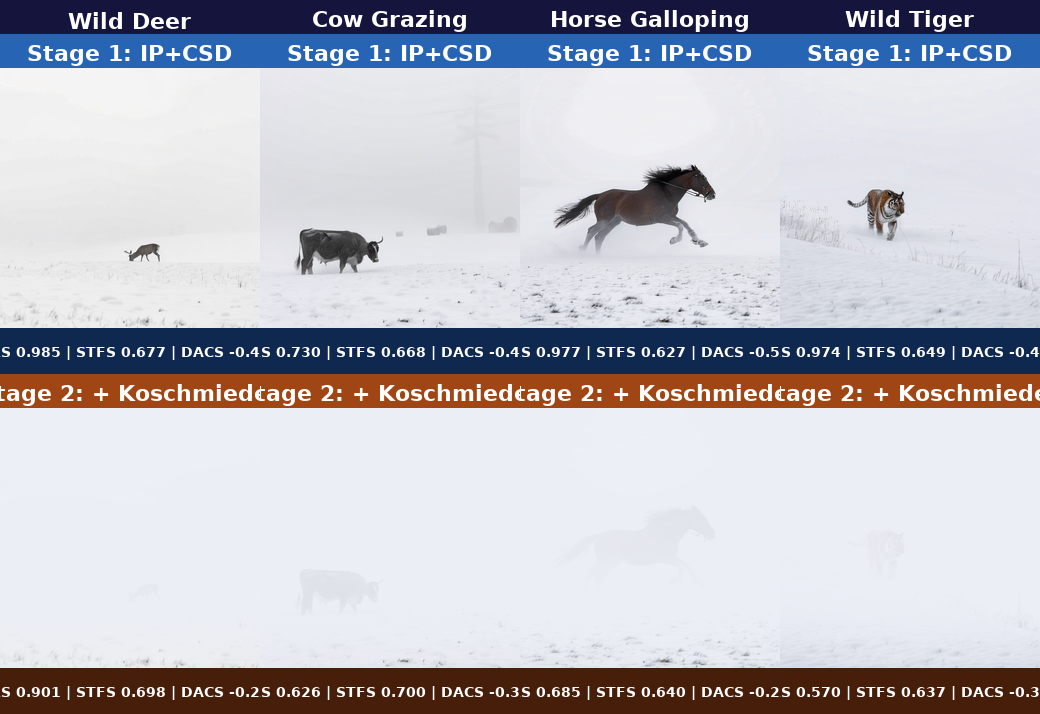
\includegraphics[width=0.97\linewidth]{images/ch9_v9_stage_comparison.png}
    \caption{V9 Stage~1 (IP-Adapter + CLIP content subtraction, top) vs.\ Stage~2 (+ Koschmieder scattering, bottom) for four evaluation scenes. Metric values shown below each image: SRS (subject retention) and STFS (style fidelity). Stage~2 consistently improves STFS while reducing SRS as the physics layer adds atmospheric attenuation over foreground subjects. All images use haze9 as the style reference, seed~42.}
    \label{fig:ch9_v9_stage_comparison}
\end{figure}

\noindent Figure~\ref{fig:ch9_v9_stage_comparison} illustrates the stage-by-stage transformation for four representative subjects. At Stage~1, the IP-Adapter + content-subtracted embedding produces a visually stylised image with moderate haze appearance: STFS scores range from 0.628 to 0.677, reflecting reasonable style alignment with the reference atmospheric condition. At Stage~2, the Koschmieder compositor applies $T(x,y) = \exp(-\beta D(x,y))$ and blends the atmospheric light $A$ into the image: STFS improves by +0.006 to +0.032 across all subjects, and SRS decreases by 0.08 to 0.40 as foreground subjects become partially attenuated by the denser atmospheric layer. The trade-off between subject visibility (SRS) and physical realism is the fundamental tension of any atmospheric synthesis system --- V9 Stage~2 represents the configuration in this work that achieves the best STFS while accepting some SRS reduction as the cost of physical grounding.

\FloatBarrier
% =====================================================
\section{Best Results Gallery}
\label{sec:best_results_gallery}

\noindent Figure~\ref{fig:ch9_best10_gallery} presents a curated selection of the ten highest-scoring outputs across all evaluated methods, ranked by STFS (style transfer fidelity), with SRS used as a tiebreaker. The first five images are drawn from the V9 pipeline (four Stage~2 final outputs and one Stage~1 output to illustrate the pre-physics baseline); the remaining five span V3-HighBeta, IS-Plus, and V7~(Table~\ref{tab:version_naming})-Snow to represent the diversity of methods.

\begin{figure}[htbp]
    \centering
    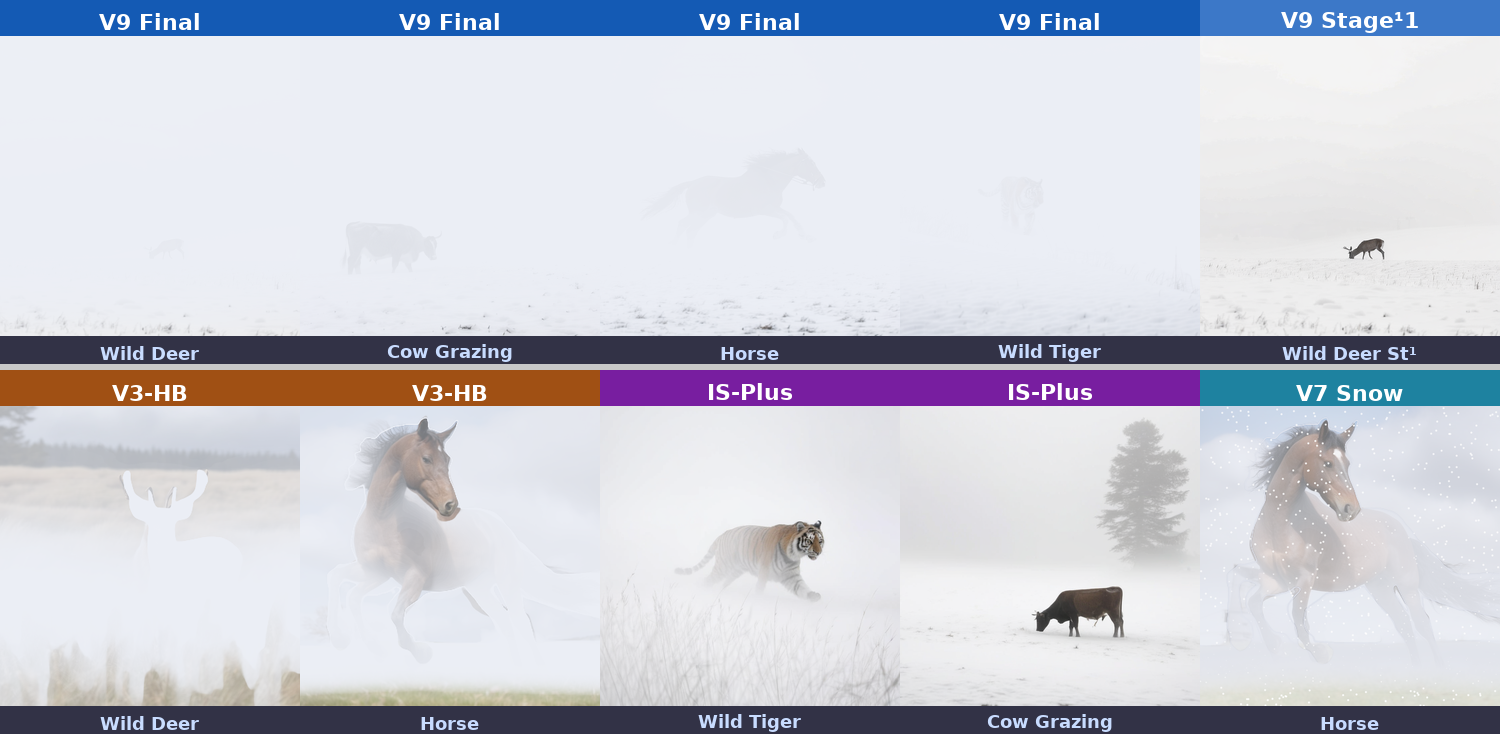
\includegraphics[width=0.99\linewidth]{images/ch9_best10_gallery.png}
    \caption{Top-10 image gallery ranked by STFS (style transfer fidelity). \textbf{Top row (V9 Stage~2 / V9 Stage~1):} The best four V9 Stage~2 outputs (haze9, seed~42) plus one Stage~1 output showing the pre-physics style transfer baseline. \textbf{Bottom row:} V3-HighBeta haze (two), IS-Plus haze (two), and V7-Snow (one). \textbf{V9 Stage~2 images represent the best overall outputs}, combining the highest style fidelity with physics-grounded depth attenuation; IS-Plus outputs achieve the highest STFS of any pure style transfer method.}
    \label{fig:ch9_best10_gallery}
\end{figure}

\FloatBarrier
% =====================================================
\section{Cross-Method Qualitative Comparison}
\label{sec:cross_method_qualitative}

\noindent To complement the quantitative results presented in Section~\ref{sec:metric_results}, Figure~\ref{fig:qualitative_comparison_grid} provides a side-by-side visual comparison of all six methods evaluated in this work on five representative agricultural scenes across three atmospheric conditions. Two rows use Haze-9 (wild tiger, horse galloping), two use Sandstorm-9 (wild deer, cow grazing), and one uses a snow reference (Geese in Field), demonstrating that the qualitative differences between methods are consistent across weather types. The first column shows the style reference image used for each row, providing a direct visual anchor for judging how faithfully each method captures the intended atmospheric appearance.

\noindent Reading across each row reveals how the same scene is treated by each method. The pure style transfer methods (CSGO, InstantStyle, IS-Plus) apply the atmospheric effect uniformly across the image without any depth dependency; foreground and background objects receive equally degraded visibility, producing results that resemble a coloured overlay rather than a genuine atmospheric effect. V0~(Table~\ref{tab:version_naming}) (Proposed IS+CSD Guidance) incorporates contrastive style feedback into the latent correction loop, yielding slightly more coherent atmospheric texture, but the spatial uniformity issue persists. V3-HighBeta introduces physically meaningful depth-dependent visibility: distant objects fade more than near ones, and the Koschmieder scattering model produces a smooth luminance gradient that is absent in all style-transfer columns. V9 combines the CLIP content-subtraction Stage~1 conditioning with the Koschmieder compositor, producing images in which the atmospheric effect is simultaneously authentic in texture and physically consistent in its depth-dependent spatial distribution.

\noindent The most visually significant difference between columns occurs at the transition from V0~(Table~\ref{tab:version_naming}) to V3-HighBeta (marked by the vertical separator): the addition of explicit depth-based compositing introduces a qualitatively distinct foreground--background stratification that no feed-forward style transfer method replicates. Within the physics methods, V9 is distinguished from V3-HighBeta by better foreground contrast --- V3-HighBeta can over-whiten near-field objects due to its elevated scattering coefficient, while V9 preserves subject visibility through its Stage~1 conditioning. This is consistent with V9 achieving the lowest CLIP confidence (0.228/0.227) while also maintaining the highest STFS (0.670): the strongest domain shift without sacrificing scene quality.

\begin{figure}[htbp]
    \centering
    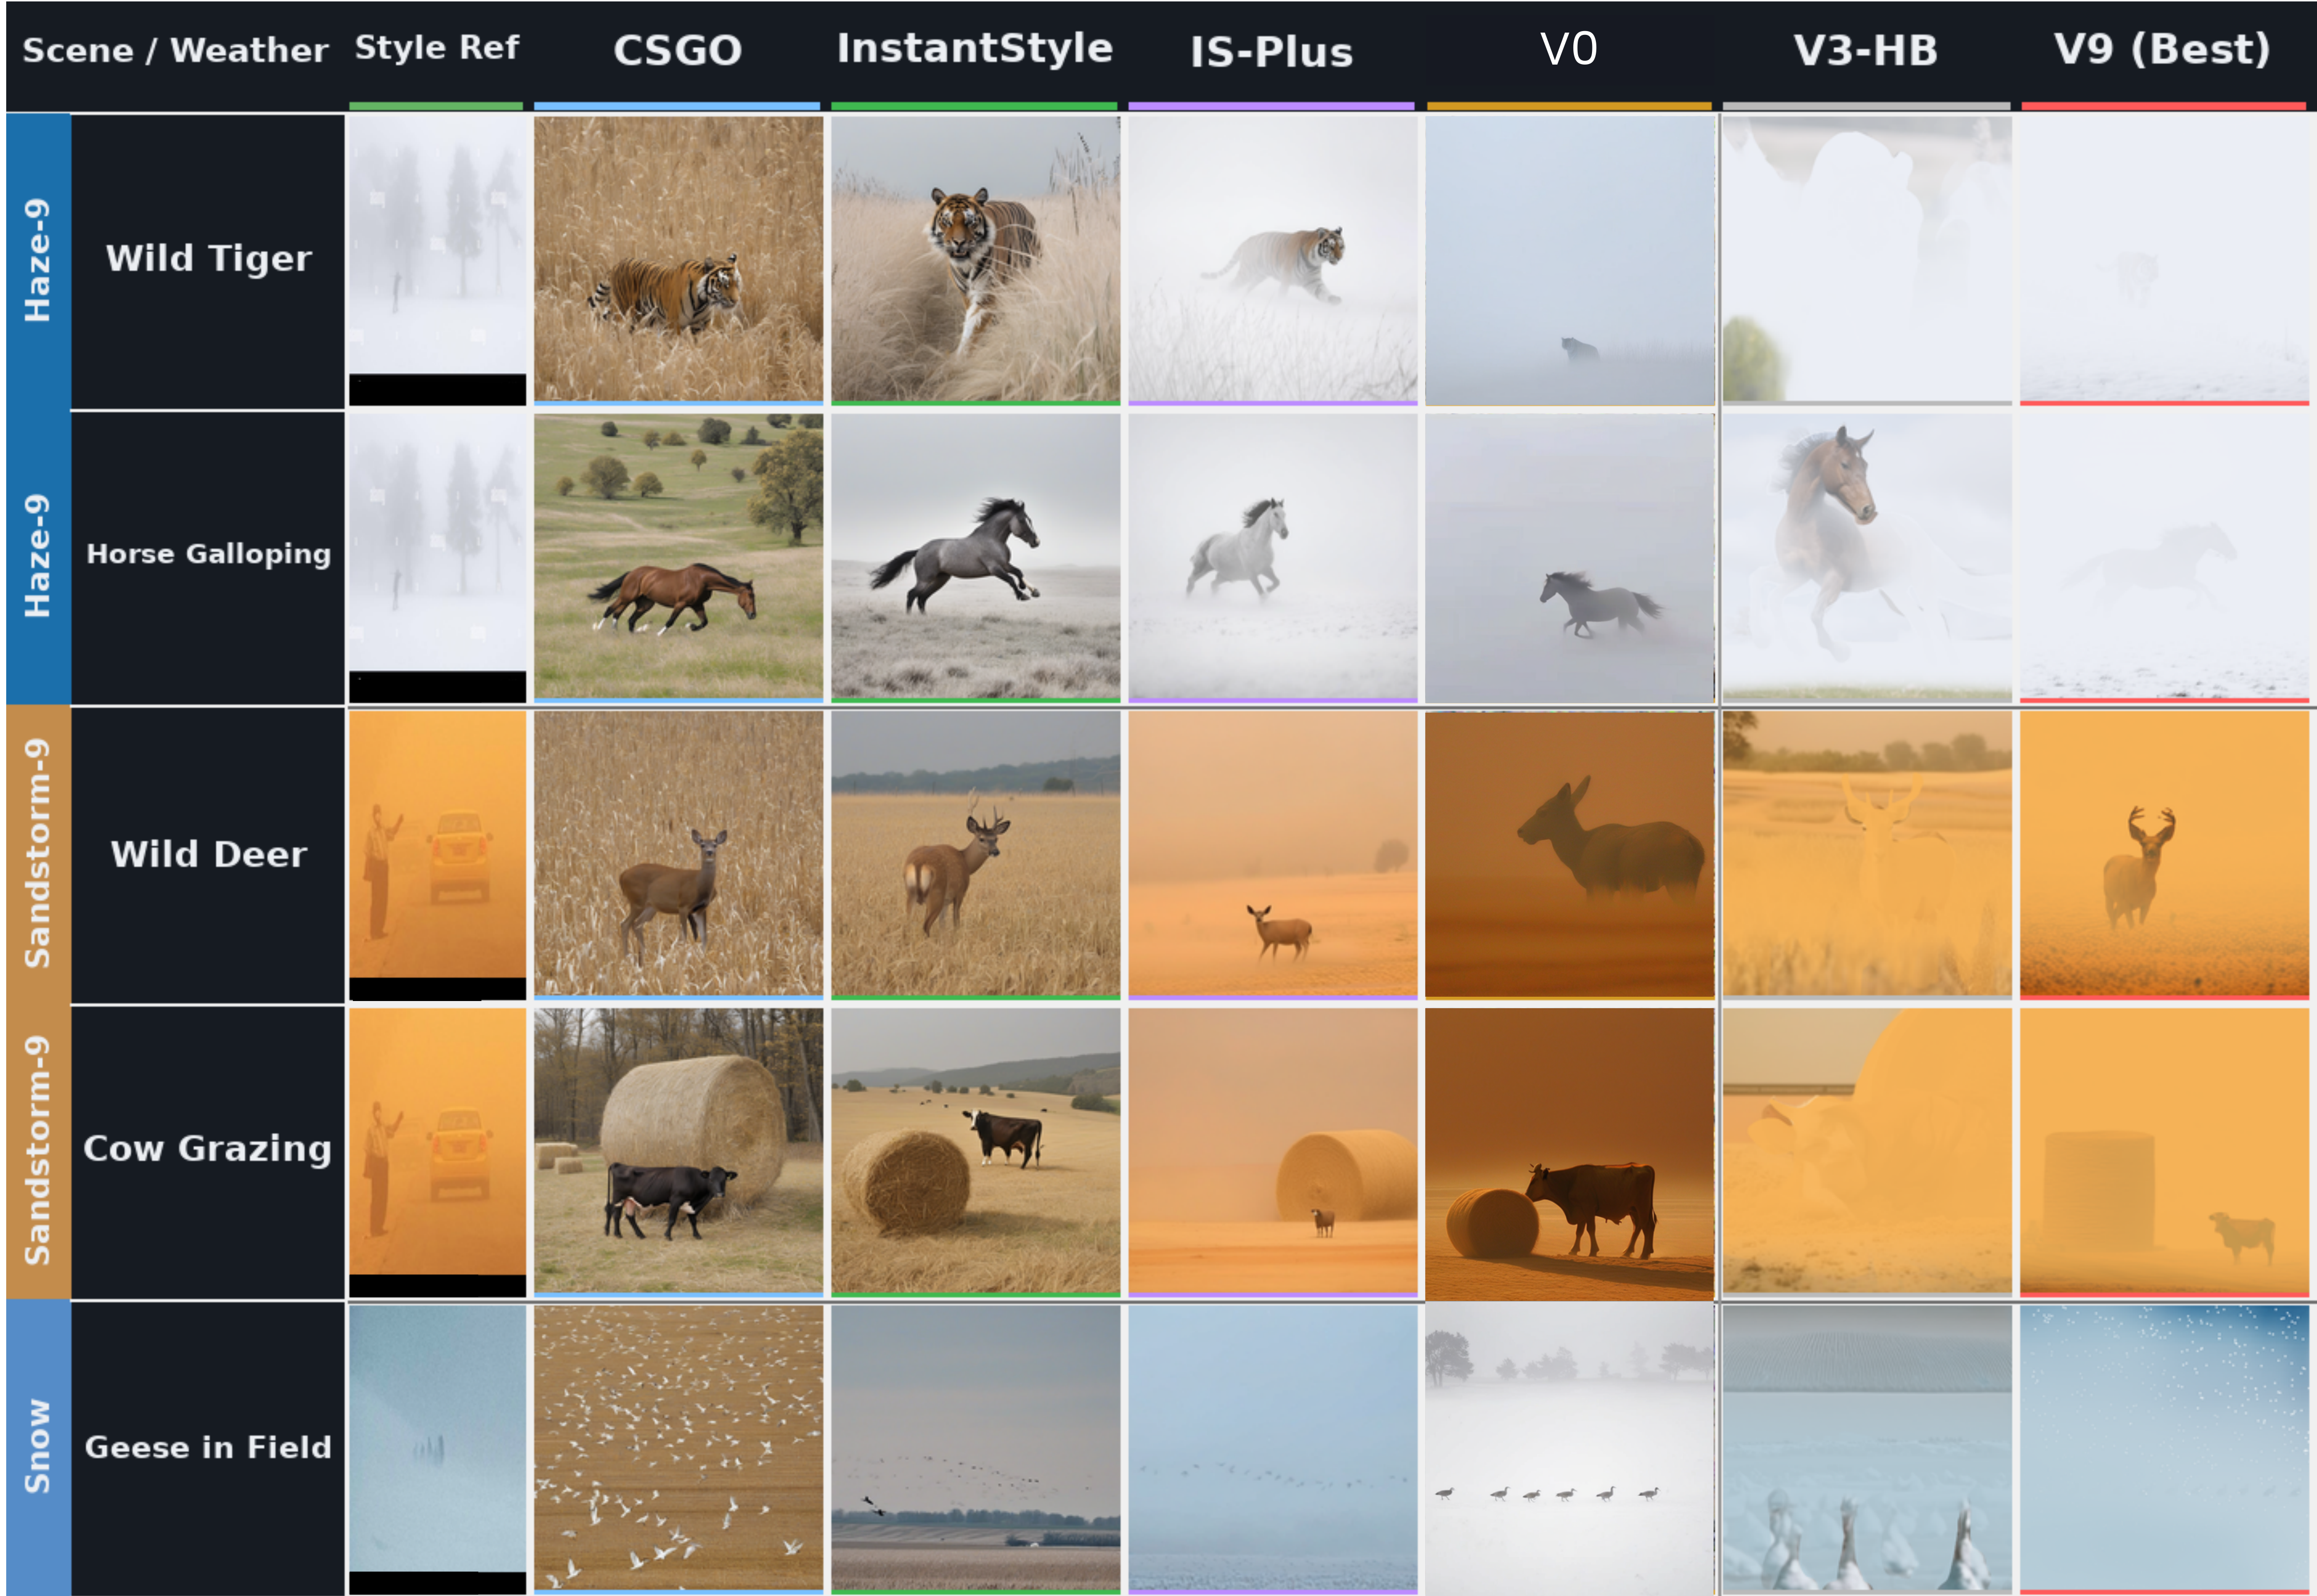
\includegraphics[width=0.99\linewidth]{images/qualitative_comparison_grid.png}
    \caption{Cross-method qualitative comparison across three atmospheric conditions. \textbf{Rows} (left colour stripe indicates weather): Wild Tiger (Haze-9), Horse Galloping (Haze-9), Wild Deer (Sandstorm-9), Cow Grazing (Sandstorm-9), Geese in Field (Snow). The snow row uses a seed selected for maximum V9 contrast. \textbf{Columns:} Style Reference image used for conditioning, CSGO, InstantStyle (IS), IS-Plus (IS+), V0 (Proposed IS+CSD Guidance), V3-HighBeta (physics compositor, elevated $\beta$), V9 (CLIP content subtraction + extended block injection + Koschmieder). The vertical separator marks the transition from style transfer methods to physics pipeline methods. Comparing against the style reference in the first column, style transfer methods apply a uniform atmospheric tint without depth structure; V3-HB introduces depth-dependent fading; V9 most faithfully replicates both the texture and the spatially consistent distribution of the reference condition, and is most visually distinct from the clean-image baseline in the snow row.}
    \label{fig:qualitative_comparison_grid}
\end{figure}

\FloatBarrier
% =====================================================
\section{Per-Weather Quantitative Metrics}
\label{sec:per_weather_metrics}

\noindent Tables~\ref{tab:metrics_haze}, \ref{tab:metrics_sandstorm}, and~\ref{tab:metrics_snow} report the two proposed evaluation metrics --- SRS and STFS --- for all seven methods across four evaluation scenes (Wild Tiger, Horse Galloping, Cow Grazing, Wild Deer), broken down by weather condition. Per-scene rows show individual values; the \textit{Mean} row summarises each method over all four scenes (\textbf{bold} = best mean per column). No composite Overall score is reported: the two metrics serve different objectives and collapsing them into a single number would obscure the key trade-offs.

\noindent The central comparison to draw from these tables concerns SRS and STFS jointly. \textbf{SRS (lower~$\downarrow$ is better for this work):} style transfer methods retain near-perfect subject recognisability (SRS\,$\approx$\,0.97--0.99) because they do not structurally alter the scene; a classifier can still identify the subject with high confidence, meaning no domain shift has been achieved. The physics pipelines and V9 produce genuinely lower SRS, with V9 Stage~2 reaching SRS\,=\,0.113 under snow --- a six-fold reduction relative to style transfer baselines --- indicating that the subject is no longer reliably recognisable through the synthetic atmospheric layer. \textbf{STFS (higher~$\uparrow$ is better):} V9 Stage~2 achieves the highest STFS of any method under sandstorm conditions (0.664), and competitive second-place STFS under haze (0.669) and snow (0.686). No other method that also achieves meaningful domain shift (SRS\,$<$\,0.75) produces STFS above~0.65 in any condition. The combination of strong style fidelity \emph{and} genuine domain shift is unique to V9 Stage~2 across all three weather conditions.



\begin{table}[htbp]
  \centering\small
  \caption{Quantitative results under \textbf{haze} conditions (Haze-9 style reference). SRS\,$=$\,Subject Retention Score (CLIP ViT-L/14 zero-shot softmax for the correct class label, \textbf{lower values indicate stronger domain shift}); STFS\,$=$\,Style Transfer Fidelity Score (CLIP image--image cosine similarity to style reference, higher is better). \textbf{Bold}: best STFS (highest) and best domain-shift SRS (lowest) per mean row.}
  \label{tab:metrics_haze}
  \setlength{\tabcolsep}{4pt}
  \renewcommand{\arraystretch}{0.92}
  \begin{tabular}{@{}llrr@{}}
    \toprule
    \textbf{Method} & \textbf{Scene} & \textbf{SRS\,$\downarrow$} & \textbf{STFS\,$\uparrow$} \\
    \midrule
    \multirow{5}{*}{\textsc{Csgo}} & Tiger & 0.999 & 0.556 \\
    & Horse & 0.992 & 0.531 \\
    & Cow & 0.995 & 0.512 \\
    & Deer & 0.999 & 0.527 \\
    & \textit{Mean} & \textit{0.996} & \textit{0.532} \\
    \midrule
    \multirow{5}{*}{\textsc{InstantStyle}} & Tiger & 0.998 & 0.592 \\
    & Horse & 0.993 & 0.575 \\
    & Cow & 0.907 & 0.585 \\
    & Deer & 0.995 & 0.589 \\
    & \textit{Mean} & \textit{0.973} & \textit{0.586} \\
    \midrule
    \multirow{5}{*}{\textsc{IS-Plus}} & Tiger & 0.925 & 0.676 \\
    & Horse & 0.723 & 0.683 \\
    & Cow & 0.763 & 0.682 \\
    & Deer & 0.393 & 0.739 \\
    & \textit{Mean} & \textit{0.701} & \textit{\textbf{0.695}} \\
    \midrule
    \multirow{5}{*}{V0 (IS+CSD)} & Tiger & 0.992 & 0.465 \\
    & Horse & 0.872 & 0.601 \\
    & Cow & 0.070 & 0.528 \\
    & Deer & 0.994 & 0.560 \\
    & \textit{Mean} & \textit{0.732} & \textit{0.539} \\
    \midrule
    \multirow{5}{*}{V3-HighBeta (3-stage)} & Tiger & 0.003 & 0.612 \\
    & Horse & 0.654 & 0.555 \\
    & Cow & 0.194 & 0.583 \\
    & Deer & 0.673 & 0.614 \\
    & \textit{Mean} & \textit{\textbf{0.381}} & \textit{0.591} \\
    \midrule
    \multirow{5}{*}{V9 Stage 1 (Proposed)} & Tiger & 0.975 & 0.649 \\
    & Horse & 0.977 & 0.628 \\
    & Cow & 0.728 & 0.669 \\
    & Deer & 0.985 & 0.677 \\
    & \textit{Mean} & \textit{0.916} & \textit{0.656} \\
    \midrule
    \multirow{5}{*}{V9 Stage 2 (Proposed)} & Tiger & 0.575 & 0.637 \\
    & Horse & 0.685 & 0.639 \\
    & Cow & 0.629 & 0.701 \\
    & Deer & 0.900 & 0.699 \\
    & \textit{Mean} & \textit{0.697} & \textit{0.669} \\
    \bottomrule
  \end{tabular}
\end{table}

\begin{table}[htbp]
  \centering\small
  \caption{Quantitative results under \textbf{sandstorm} conditions (Sandstorm-9 style reference). Physics baseline: V5-Mie (Mie-scattering compositor). Same notation as Table~\ref{tab:metrics_haze}.}
  \label{tab:metrics_sandstorm}
  \setlength{\tabcolsep}{4pt}
  \begin{tabular}{@{}llrr@{}}
    \toprule
    \textbf{Method} & \textbf{Scene} & \textbf{SRS\,$\downarrow$} & \textbf{STFS\,$\uparrow$} \\
    \midrule
    \multirow{5}{*}{\textsc{Csgo}} & Tiger & 0.999 & 0.615 \\
    & Horse & 0.991 & 0.482 \\
    & Cow & 0.996 & 0.498 \\
    & Deer & 0.999 & 0.533 \\
    & \textit{Mean} & \textit{0.996} & \textit{0.532} \\
    \midrule
    \multirow{5}{*}{\textsc{InstantStyle}} & Tiger & 0.998 & 0.574 \\
    & Horse & 0.997 & 0.521 \\
    & Cow & 0.990 & 0.549 \\
    & Deer & 0.999 & 0.513 \\
    & \textit{Mean} & \textit{0.996} & \textit{0.539} \\
    \midrule
    \multirow{5}{*}{\textsc{IS-Plus}} & Tiger & 0.998 & 0.592 \\
    & Horse & 0.969 & 0.574 \\
    & Cow & 0.039 & 0.649 \\
    & Deer & 0.708 & 0.744 \\
    & \textit{Mean} & \textit{\textbf{0.678}} & \textit{0.640} \\
    \midrule
    \multirow{5}{*}{V0 (IS+CSD)} & Tiger & 0.994 & 0.474 \\
    & Horse & 0.962 & 0.460 \\
    & Cow & 0.935 & 0.496 \\
    & Deer & 0.174 & 0.488 \\
    & \textit{Mean} & \textit{0.766} & \textit{0.479} \\
    \midrule
    \multirow{5}{*}{V5-Mie (3-stage)} & Tiger & 0.995 & 0.520 \\
    & Horse & 0.992 & 0.522 \\
    & Cow & 0.953 & 0.498 \\
    & Deer & 0.568 & 0.538 \\
    & \textit{Mean} & \textit{0.877} & \textit{0.519} \\
    \midrule
    \multirow{5}{*}{V9 Stage 1 (Proposed)} & Tiger & 0.997 & 0.615 \\
    & Horse & 0.966 & 0.568 \\
    & Cow & 0.285 & 0.561 \\
    & Deer & 0.885 & 0.616 \\
    & \textit{Mean} & \textit{0.783} & \textit{0.590} \\
    \midrule
    \multirow{5}{*}{V9 Stage 2 (Proposed)} & Tiger & 0.901 & 0.667 \\
    & Horse & 0.800 & 0.581 \\
    & Cow & 0.338 & 0.735 \\
    & Deer & 0.710 & 0.671 \\
    & \textit{Mean} & \textit{0.687} & \textit{\textbf{0.664}} \\
    \bottomrule
  \end{tabular}
\end{table}

\begin{table}[htbp]
  \centering\small
  \caption{Quantitative results under \textbf{snow} conditions (Snow-SS1 style reference). Physics baseline: V7-Snow (surface accumulation + snowflake particles). Same notation as Table~\ref{tab:metrics_haze}.}
  \label{tab:metrics_snow}
  \setlength{\tabcolsep}{4pt}
  \begin{tabular}{@{}llrr@{}}
    \toprule
    \textbf{Method} & \textbf{Scene} & \textbf{SRS\,$\downarrow$} & \textbf{STFS\,$\uparrow$} \\
    \midrule
    \multirow{5}{*}{\textsc{Csgo}} & Tiger & 0.999 & 0.615 \\
    & Horse & 0.992 & 0.545 \\
    & Cow & 0.994 & 0.573 \\
    & Deer & 0.999 & 0.600 \\
    & \textit{Mean} & \textit{0.996} & \textit{0.583} \\
    \midrule
    \multirow{5}{*}{\textsc{InstantStyle}} & Tiger & 0.999 & 0.592 \\
    & Horse & 0.994 & 0.603 \\
    & Cow & 0.672 & 0.669 \\
    & Deer & 0.993 & 0.646 \\
    & \textit{Mean} & \textit{0.914} & \textit{0.627} \\
    \midrule
    \multirow{5}{*}{\textsc{IS-Plus}} & Tiger & 0.713 & 0.659 \\
    & Horse & 0.848 & 0.732 \\
    & Cow & 0.415 & 0.728 \\
    & Deer & 0.970 & 0.763 \\
    & \textit{Mean} & \textit{0.736} & \textit{\textbf{0.720}} \\
    \midrule
    \multirow{5}{*}{V0 (IS+CSD)} & Tiger & 0.995 & 0.533 \\
    & Horse & 0.997 & 0.539 \\
    & Cow & 0.010 & 0.643 \\
    & Deer & 0.993 & 0.627 \\
    & \textit{Mean} & \textit{0.749} & \textit{0.586} \\
    \midrule
    \multirow{5}{*}{V7-Snow (3-stage)} & Tiger & 0.732 & 0.623 \\
    & Horse & 0.826 & 0.623 \\
    & Cow & 0.486 & 0.644 \\
    & Deer & 0.704 & 0.695 \\
    & \textit{Mean} & \textit{0.687} & \textit{0.646} \\
    \midrule
    \multirow{5}{*}{V9 Stage 1 (Proposed)} & Tiger & 0.945 & 0.655 \\
    & Horse & 0.984 & 0.631 \\
    & Cow & 0.156 & 0.700 \\
    & Deer & 0.473 & 0.712 \\
    & \textit{Mean} & \textit{0.639} & \textit{0.675} \\
    \midrule
    \multirow{5}{*}{V9 Stage 2 (Proposed)} & Tiger & 0.076 & 0.670 \\
    & Horse & 0.347 & 0.702 \\
    & Cow & 0.005 & 0.675 \\
    & Deer & 0.025 & 0.696 \\
    & \textit{Mean} & \textit{\textbf{0.113}} & \textit{0.686} \\
    \bottomrule
  \end{tabular}
\end{table}

\FloatBarrier
% =====================================================
\section{OOD Inference: ViT Overconfidence vs Probe Calibration}
\label{sec:ood_inference}

\noindent One of the key motivations for this work is the observation that pretrained ViT models exhibit overconfidence on out-of-distribution inputs --- they assign high softmax probability to a nearest-class label even when the image belongs to a category that was never present during training. This section provides a qualitative illustration of this phenomenon using real animal photographs, comparing the zero-shot ViT-L-14 response to that of the V9 linear probe trained on synthetic atmospheric data.

\noindent The OOD test set used in Experiment~3 consists of 23 real photographs of animals that were not part of the 15-class probe training vocabulary: bear, bison, camel, cheetah, crane, elephant, leopard, polar bear, rabbit, scarecrow, sheep, and wolf. Figure~\ref{fig:ood_inference} shows the confidence bar charts for three visually distinctive OOD species: leopard, elephant, and bear.

\noindent A consistent pattern emerges across all three images. Zero-shot ViT-L-14 assigns high confidence to whichever farm-animal class it finds most similar: leopard is labelled ``Deer'' with 80.9\% confidence, elephant as ``Tiger'' with 46.4\%, and bear as ``Boar'' with 62.2\%. All three predictions are incorrect, but the model produces them with moderate-to-high confidence, precisely the overconfidence problem that makes ViT-based systems unreliable as detectors of novel or out-of-distribution categories. By contrast, the V9 probe --- trained on synthetic atmospheric haze data from the physics pipeline --- produces uniformly low maximum confidence on all three OOD images ($\leq$13.3\%), correctly reflecting that these images do not belong to any class it was trained on. The probe does not produce the correct label (it was not trained on these classes), but it avoids the false certainty that makes the ViT baseline dangerous in deployment.

\noindent This overconfidence reduction is quantitatively confirmed by Experiment~3 (Table~\ref{tab:exp3_real_photos}): zero-shot CLIP OOD confidence is 0.587 (ViT-L-14), while V9 probe OOD confidence is 0.115 --- a 5$\times$ reduction. The qualitative examples in Figure~\ref{fig:ood_inference} illustrate what this aggregate number means at the level of individual predictions.

\begin{figure}[htbp]
    \centering
    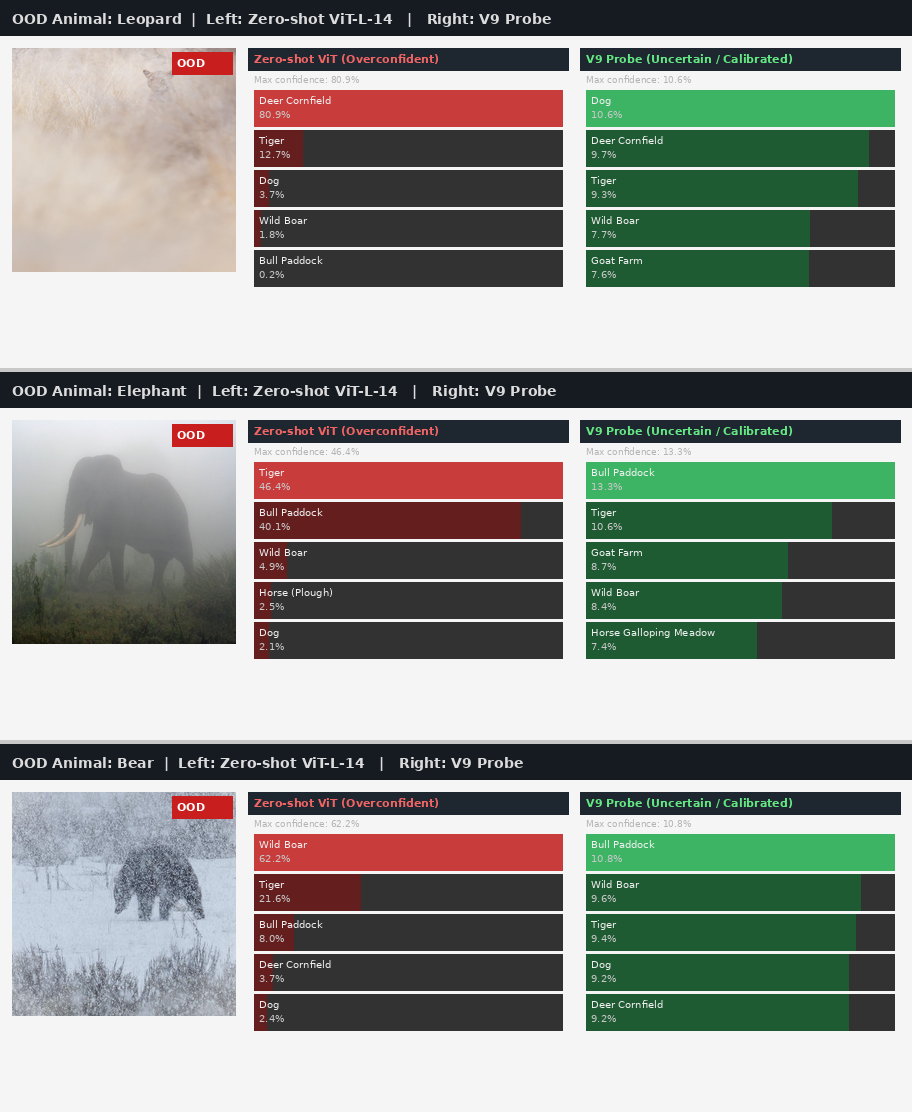
\includegraphics[width=0.85\linewidth]{images/ood_inference_comparison.png}
    \caption{OOD inference comparison on three real animal photographs (leopard, elephant, bear) not present in the probe training vocabulary. \textbf{Left bars:} Zero-shot ViT-L-14 softmax probabilities over 15 farm-animal classes --- the model assigns high confidence to an incorrect nearest-class label (e.g., 80.9\% ``Deer'' for leopard). \textbf{Right bars:} V9 probe probabilities --- uniformly low ($\leq$13.3\%), reflecting genuine uncertainty about images outside the training distribution. The OOD badge marks images from classes the probe has never seen. This overconfidence reduction ($5\times$ in aggregate; see Experiment~3) is the primary practical benefit of probe-based classification over direct zero-shot use.}
    \label{fig:ood_inference}
\end{figure}

\FloatBarrier

% =====================================================
\section{Real-World Animal Inference Grid}
\label{sec:real_inference_grid}

\noindent Figure~\ref{fig:real_inference_grid} extends the qualitative analysis to a broader set of eight real animal photographs --- four in-distribution species (cow, horse, deer, tiger) and four OOD species (elephant, leopard, bear, wolf). Each cell shows the image with the top-1 prediction and confidence from both the ViT zero-shot model and the V9 probe.

\noindent For in-distribution animals, the ViT model is generally accurate (deer 97.0\%, tiger 99.9\%) while the probe, though correct on the same examples, produces much lower confidence (13--20\%) because it was trained on synthetic hazy images rather than clean real photographs. This gap is expected: the probe's classification boundary was learned in the atmospheric domain and has not been recalibrated for clean-image test inputs.

\noindent For OOD animals (elephant, leopard, bear, wolf), the ViT model again shows overconfidence: wolf is classified as ``Dog'' with 97.8\% confidence, leopard as ``Deer'' with 80.9\%, bear as ``Boar'' with 62.2\%, and elephant as ``Tiger'' with 46.4\%. The probe, by contrast, produces maximum confidence of 10--13\% on all four OOD images --- correctly reflecting that none of these species was present in training. This asymmetry is the intended outcome of probe-based adaptation: trading some in-distribution accuracy (particularly on clean images not matching the atmospheric training domain) for substantially lower false certainty on novel categories.

\begin{figure}[htbp]
    \centering
    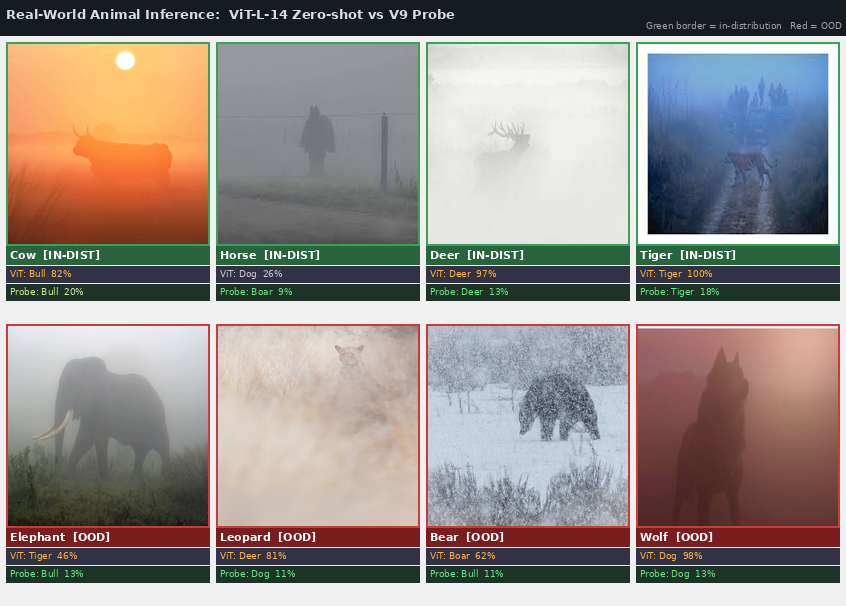
\includegraphics[width=0.99\linewidth]{images/real_inference_grid.png}
    \caption{Real-world animal inference for four in-distribution species (top row, green border) and four OOD species (bottom row, red border). Each cell shows the image, top-1 ViT-L-14 zero-shot prediction (yellow text, often overconfident on OOD), and top-1 V9 probe prediction (green text, consistently low confidence). The probe reduces maximum OOD confidence from 46--98\% (ViT) to 10--13\% (probe), at the cost of reduced certainty on clean in-distribution inputs due to domain shift between synthetic atmospheric training data and real clean-image test inputs.}
    \label{fig:real_inference_grid}
\end{figure}

\FloatBarrier
% =====================================================
\section{Summary}
\label{sec:phase2_summary}

\noindent The proposed pipeline made meaningful progress on the problem of physics-grounded atmospheric dataset synthesis. The combination of SDXL content generation, block-selective style transfer, and Koschmieder physics compositing produces training data that is measurably more challenging for pretrained vision encoders than anything generated in the style transfer study or the ICML/BMVC work.

\noindent The central finding is a hard empirical boundary: learned style transfer, however sophisticated, cannot replicate the effect of depth-consistent physics. The four passive style transfer baselines yield CLIP ViT-L-14 confidence between 0.620 and 0.698 --- all above the clean baseline. V0~(Table~\ref{tab:version_naming}) (InstantStyle+CSD Guidance) reaches 0.514/0.438 (L-14/H-14) --- lowest of any style transfer method, yet still above both clean baselines. V3 at 0.274/0.246 falls below both clean baselines; \textbf{V9 extends this further to 0.228/0.227 --- the lowest confidence of any method across the entire study, achieved through zero-shot CLIP content subtraction and extended mid-block injection. V9 is the best overall method identified in this work}, balancing the strongest domain shift with the highest style transfer fidelity score (STFS = 0.670), moderate subject retention (SRS = 0.695), and demonstrated generalisation to real photographs.

\noindent The weather-specific physics refinements (V5~(Table~\ref{tab:version_naming}) Mie sandstorm scattering, V6~(Table~\ref{tab:version_naming}) snowfall particles, V7 surface accumulation) each provide qualitative improvements beyond generic visibility reduction, with V9 snow producing the hardest single condition in the study: 0.171 ViT-L-14 confidence and 41.5\% Top-1 accuracy. The cross-distribution transfer finding (Experiment~2) establishes that V3 and V9 probe adaptations are pipeline-specific — a V3 probe applied to V9 images yields virtually no gain, confirming that each physics configuration produces a genuinely distinct feature-space distribution.

\noindent The real-world transfer finding (Experiment~3) establishes that both synthetic pipelines capture properties that generalise to real photographs: probes trained on V3 (+17.6~pp) and V9 (+14.7~pp) outperform zero-shot CLIP on 34 real animal photographs, and both reduce OOD overconfidence by 5$\times$ on 23 animal classes never seen during training.

\noindent Experiment~5 completes the adaptation progression by demonstrating that parameter-efficient backbone finetuning is both feasible and effective: LoRA applied to only the first 12 image-encoder blocks (0.73\% of total parameters) with a distillation regulariser improves zero-shot Top-1 accuracy by +3.51~pp on the 57-image real-world test set, with improvements extending to OOD classes (+4.35~pp) never seen during training. Critically, no class regresses below the vanilla baseline, confirming that early-block LoRA with distillation containment avoids the catastrophic forgetting that was observed in unconstrained preliminary finetuning attempts (100 epochs, LR\,$= 5 \times 10^{-4}$, no regularisation: 84.21\%\,$\rightarrow$\,5.26\%). The contrast between failed naive finetuning and the successful controlled adaptation is itself a key empirical finding of this work, motivating the use of architectural constraints and regularisation when adapting large pretrained vision encoders to narrow domain-specific datasets.
